\documentclass[]{scrreprt}
% \KOMAoptions{fontsize=14pt}

\usepackage{amsmath,amsfonts,amssymb,amsthm,mathtools} % AMS

\usepackage{hyperref}       % hyperref
\hypersetup{				% settings
	unicode=true,           % non-latin letters
	pdftitle={Practical application of the Wilcoxon-Mann-Whitney test in valuation
},   % heading
	pdfauthor={K. A. Murashev},      % Author
	pdfsubject={Wilcoxon-Mann-Whitney test},      % Scope
	pdfcreator={K. A. Murashev}, % Creator
	pdfproducer={K. A. Murashev}, % Producer
	pdfkeywords={Wilcoxon-Mann-Whitney test, U-test} % Keywords
	colorlinks=true,       	% false: links in frames; true: coloured links
	linkcolor=red,          % internal links
	citecolor=green,        % bibliography links
	filecolor=magenta,      % file links
	urlcolor=blue           % URL links
}

\usepackage{url}

\usepackage{babel}

% work with images
\usepackage{graphicx}
\graphicspath{{Images/}}

% work with tables
\usepackage{array, tabularx, tabulary, booktabs, xtab} % additional forms of tables
\usepackage{longtable}  % long tables
\usepackage{multirow} % merge rows

% work with bibliography
\usepackage[backend=biber,bibencoding=utf8,sorting=ynt,maxcitenames=5,sortupper=true,date=iso]{biblatex}

% set the depth of table of contents
\setcounter{tocdepth}{8}

% work with scripts
\usepackage {listings}
\lstloadlanguages{[Latex]Tex, bash, R, Python, SQL}
\lstset{extendedchars=true , % additional symbols
frame=tb, % top & bottom frames
commentstyle=\itshape , % font for comments
stringstyle =\ttfamily % font for 'strings'
keywordstyle=\color{blue} % color for keywords
}

% connecting the automated bibliography package
\usepackage[backend=biber,bibencoding=utf8,sorting=ynt,maxcitenames=5,sortupper=true,date=iso]{biblatex} 

% add sources for bibliography
\addbibresource{/home/kaarlahti/TresoritDrive/Methodics/My/AI_for_valuers/Book/AI_for_valuers_book/Basic_principles.bib}
\addbibresource{/home/kaarlahti/TresoritDrive/Methodics/My/AI_for_valuers/Book/AI_for_valuers_book/LaTeX.bib}
\addbibresource{/home/kaarlahti/TresoritDrive/Methodics/My/AI_for_valuers/Book/AI_for_valuers_book/Mathstat.bib}
\addbibresource{/home/kaarlahti/TresoritDrive/Methodics/My/AI_for_valuers/Book/AI_for_valuers_book/Murashev.bib}
\addbibresource{/home/kaarlahti/TresoritDrive/Methodics/My/AI_for_valuers/Book/AI_for_valuers_book/Python.bib}
\addbibresource{/home/kaarlahti/TresoritDrive/Methodics/My/AI_for_valuers/Book/AI_for_valuers_book/R.bib}
\addbibresource{/home/kaarlahti/TresoritDrive/Methodics/My/AI_for_valuers/Book/AI_for_valuers_book/RussianLaws.bib}
\addbibresource{/home/kaarlahti/TresoritDrive/Methodics/My/AI_for_valuers/Book/AI_for_valuers_book/Sci&Tech.bib}
\addbibresource{/home/kaarlahti/TresoritDrive/Methodics/My/AI_for_valuers/Book/AI_for_valuers_book/Valuation.bib}
\addbibresource{/home/kaarlahti/TresoritDrive/Methodics/My/AI_for_valuers/Book/AI_for_valuers_book/ValuationStandards.bib}
\addbibresource{/home/kaarlahti/TresoritDrive/Methodics/My/AI_for_valuers/Book/AI_for_valuers_book/ZHZL.bib}

\usepackage{bbm} % indicator function

\newcommand{\github}{
	{%
		
\includegraphics[width=3ex,height=3ex,keepaspectratio]{github-seeklogo.pdf}
}
}


% Title Page
\title{Practical application of~the~Wilcoxon-Mann-Whitney test in~valuation.}
\subtitle{Selection of~attributes as~pricing factors based on~the~principle of~unbiased estimates}
\author{\href{https://www.facebook.com/groups/1977067932456703}{K.~A.~Murashev}}

\begin{document}
\maketitle
%
\lstset{language=Python,
	basicstyle=\ttfamily,
	keywordstyle=\color{Blue}\ttfamily,
	stringstyle=\color{Red}\ttfamily,
	commentstyle=\color{Emerald}\ttfamily,
	morecomment=[l][\color{Magenta}]{\#},
	breaklines=true,
	breakindent=0pt,
	breakatwhitespace,
	columns=fullflexible,
	showstringspaces=false
}
%	
\begin{abstract}
	Appraisers often face the need to take into account differences in quantitative and qualitative characteristics of objects in their practice. In particular, one of the standard tasks is to determine the attributes that influence the cost (so-called "pricing factors") and to separate them from the attributes that do not or cannot~be determined.
	
	Subjective selection of~attributes taken into account in~determining the~value is~widespread in~valuation practice. In~this case, specific quantitative indicators of~the~impact of~these attributes on~the~cost are~often taken from the~so-called "reference books". While not~denying the~speed and~low cost of~this approach, it~should~be recognized that only data directly observed in~the open markets is~a~reliable basis for~a~value judgment. The priority of~such data over other data, in~particular those obtained by~expert survey, is~enshrined, among others, in~\href{https://www.rics.org/uk/upholding-professional-standards/sector-standards/valuation/red-book/red-book-global/}{RICS Valuation --- Global Standards 2022}~\cite{RVGS-2022}, \href{https://www.rics.org/uk/upholding-professional-standards/sector-standards/valuation/red-book/international-valuation-standards/}{International Valuation Standards 2022}~\cite{IVS-2022}, as~well as~in~\href{http://eifrs.ifrs.org/eifrs/bnstandards/en/IFRS13.pdf}{IFRS~13 "Fair Value Measurement"}~\cite{IFRS-13}. Therefore, we~can say that mathematical methods for~analyzing data from the open market are the~most reliable means of~interpreting market information used in~market research and~predicting the~value of~individual objects.
	
	The aim of~this work is~to~justify the~necessity and~possibility of~using a~rigorous mathematical Wilcoxon--Mann--Whitney test, which allows us~to~answer the~question about the~necessity of~taking into account the~binary attribute as~a~price-generating factor. Judgmental approach is most commonly used by appraisers in selecting the attributes to be considered in appraisal. But this paper proposes the idea of prioritizing the measuring approach based on the results of a mathematical test. It allows to draw a conclusion about the importance or otherwise of the binary attribute influence on the value. It~should~be noted that despite the~fact that the~statistical test under consideration belongs to~frequentist statistics, it, through its~connection to~ROC analysis and~AUC, is~related to~modern machine learning methods, which will~be discussed later in~the~text of~this material. The~presence of~this relationship and~elements of~Bayesian statistics seems particularly interesting and~promising from the~point of~view of~introducing machine learning and~data analysis methods into the~everyday practice of~appraisers.
	
	Users should have some general math background and~basic Python and~R programming skills to~understand and~practice all of~the material in~the~text, but~lack of~that knowledge and~skill is~not~a~barrier to~learning most of~the~material and~implementing the~test in~the~spreadsheet that comes with it.
	
	The material consists of~four blocks:
	\begin{itemize}
		\item a~description of~the~Wilcoxon--Mann--Whitney test (hereafter "U-test"), its probabilistic meaning, and~its relationship to~other mathematical methods;
		\item a~practical implementation of~the~U-test in~a~spreadsheet on~an~example of~test random data;
		\item practical implementation of~the~U-test on~the~real data of~the~residential real estate market of~St.~Petersburg agglomeration by~means of~Python programming language, the~purpose of~the~analysis was~to~check the~significance of~the~difference in~the~unit price between the~objects located in~the~urban and~suburban parts of~the~agglomeration;
		\item practical implementation of~the~U-test on~real data of~residential real estate market of~Almaty by~means of~R programming language, the~purpose of~the~analysis was~to~check the~significance of~difference in~unit price between the~objects sold without demountable improvements and~the~objects sold with them.
	\end{itemize}
	The~current version of~this material, its source code, Python and~R scripts, and~the~spreadsheet are~in~the~repository on~the GitHub portal and~are~available at~the~\href{https://github.com/Kirill-Murashev/AI_for_valuers_book/tree/main/Parts-Chapters/Mann-Whitney-Wilcoxon}{permanent link}~\cite{Murashev:u-test}.
	
	This material and~all of~its~appendices are~distributed under the~terms of~the~\href{https://creativecommons.org/licenses/by-sa/4.0/}{cc-by-sa-4.0} license~\cite{cc-by-sa-4.0}.
\end{abstract}	
%
\tableofcontents
\listoftables
\listoffigures
\lstlistoflistings
%	
\chapter{Technical details}
This material, as~well as~the~appendices to~it, are available at~\href{https://github.com/Kirill-Murashev/AI_for_valuers_book/tree/main/Parts-Chapters/Mann-Whitney-Wilcoxon}{permanent link}~\cite{Murashev:u-test}. The~source code for~this work was~created~using the~language~\href{https://www.ctan.org/}{\TeX}~\cite{TeX:site} with~a~set of~macro extensions~\href{https://www latex-project.org/}{\LaTeXe}~\cite{LaTeX:site}, distribution~\href{https://www.tug.org/texlive/}{TeXLive}~\cite{TeXLive:site} and~Editor~\href{https://www.texstudio.org/}{TeXstudio}~\cite{TeXstudio:site}. The~spreadsheet calculation was~done with \href{https://www.libreoffice.org/discover/calc/}{LibreOffice Calc}~\cite{LO:Calc} (Version: 7.3.4. 2 / LibreOffice Community Build ID: 30(Build:2); CPU threads: 4; OS: Linux 5.11; UI render: default; VCL: kf5 (cairo+xcb) Locale: en-US (en\_US.UTF-8); UI: en-US Ubuntu package version: 1:7.3.4~rc2-0ubuntu0.20.04.1~lo1; Calc: threaded). The~calculation in~\href{https://www.r-project.org/}{R}~\cite{R_language} (version 4.2.1 (2022-06-23) -- "Funny-Looking Kid") was~done~using an~IDE~\href{https://www.rstudio.com/}{RStudio} (RStudio 2022. 02.3+492 "Prairie Trillium" Release (1db809b8, 2022-05-20) for Ubuntu Bionic; Mozilla/5.0 (X11; Linux x86\_64); AppleWebKit/537.36 (KHTML, like Gecko); QtWebEngine/5.12.8; Chrome/69.0.3497.128; Safari/537.36)~\cite{RStudio:official_site}. The~calculation in~\href{https://www.python.org/}{Python}~(Version~3.9.12)~\cite{Python:site} was~performed using the~development environment~\href{https://jupyter.org}{Jupyter Lab} (Version 3.4.2)~\cite{Jupyter:site} and~IDE \href{https://www.spyder-ide.org/}{Spyder} (Spyder version: 5.1.5 None* Python version: 3.9.12 64-bit * Qt version: 5.9.7 * PyQt5 version: 5.9.2
* Operating System: Linux 5.11.0-37-generic)~\cite{Spyder:site}. The~graphics used in~the~subsection \ref{U-test-spreadsheet} were prepared using \href{Geogebra:official-site}{Geogebra}~(Version 6.0.666.0-202109211234)~\cite{Geogebra:official-site}. The~following values were used in~this material as~well as~in~most of~the~works in~the~series:
\begin{itemize}
	\item significance level: $\alpha = 0.05$;
	\item confidence interval: $Pr = 0.95$;
	\item initial position of the pseudo-random number generator: $seed=19190709$.
\end{itemize}
A~dot is~used as~a~decimal point. Most of~the~mathematical notations are~written as~they are~used in~English-speaking circles. For~example, a~tangent is~written as~$\tan$, not~$tg$. The~results of~statistical tests are~considered significant when
\begin{equation}\label{eq:significance}
p \leq \alpha.
\end{equation}
This decision is~based, in~part, on~the~results of~the~discussion that took place on~\href{researchgate.net}{researchgate.net}~~\cite{RG:p-equals-alpha}.
%
\chapter{Subject of~research}
When working with market data, the~appraiser is~often faced with the~task of~testing the~hypothesis of~whether a~quantitative, ordinal or~nominal attribute has~a~significant effect on~the~price. Real estate market analysts, developers, realtors, employees of~collateral departments of~banks, leasing and~insurance companies, tax inspectors and~other specialists have a~similar task. At~the~same time, it~is~often impossible to~collect large amounts of~data that would allow a~wide range of~machine learning methods to~be~applied. In~some cases appraisers consciously narrow the~area of~data collection to~the~narrow market segment, resulting in~only very small samples of~less than thirty observations at~their disposal. In~this case, the~price data most often has~a~distribution that differs from the~normal one. In~this case, a~rational solution is~to~use U-test. Let~us formulate the~problem:
\begin{itemize}
	\item suppose that we~have two samples of~unit prices for~commercial premises, some of~which have some attribute (e.\,g., having a~separate entrance) and~some of~which do~not;
	\item it~is~necessary to~determine whether the~presence of~this feature has a~significant impact on~the~unit value of~this type of~real estate or~not.
\end{itemize}
At~first glance, according to~established practice, an~appraiser can simply subjectively recognize some attributes as~significant and~others as~not, and~then accept the~adjustment values for~differences in~these attributes from the~reference books. However, as~mentioned above, this approach is~hardly considered best practice because it~lacks any~market analysis. Also, in~that case, it~is~unlikely that such work is~of~any~serious value at~all.

Instead, it~is~possible to~use random samples of~market data and~apply mathematical analysis to~them, allowing scientific and evidence-based conclusions to~be~drawn about the~significance of~a~particular attribute's impact on~value. The~data used in~this paper to~perform the~U-test using Python and~R are~real market data, some of~which were collected by~the author through web scraping and some provided by~colleagues for~the~analysis. The~attached spreadsheet is~set~up so~that test raw data can~be generated in~a~pseudo-random fashion.

The~subject of~this paper is~the~nonparametric Wilcoxon-Mann-Whitney test, specifically designed for~samples that have a~distribution other than normal. This circumstance is~important because the~price data that appraisers deal with most often have this distribution, which excludes the~possibility of~applying the~parametric t-criterion and~z-criterion. In~addition, the~test under consideration is~of~great interest because it~has a~connection to~machine learning methods through AUC, the~calculation of~which through the~formula provided in~the~test framework gives a~value equal to~that calculated by~ROC analysis. Thus, the~study of~the~U-test paves the~way for~a~further dive into the~world of~machine learning, which is~entering many areas of~human activity and~will significantly change the~field of~value estimation in~the~foreseeable future.

The~material contains a~description of~the~test and~instructions for~performing it, sufficient in~the~author's opinion for~its~demonstrable use in~the~estimation process.
%
\chapter{Basic information about the~test}
\section{Assumptions and~formalization of~hypotheses}
First of~all, it~should~be said that, in~spite of~the~stated common name, it~is~more correct to~speak of~two tests:
\begin{itemize}
	\item \href{http://www.machinelearning.ru/wiki/index.php?title=Критерий_Уилкоксона_двухвыборочный}{Wilcoxon rank-sum test} developed by~Frank Wilcoxon in~1945~\cite{MLRU:Wilcoxon-test};
	\item \href{http://www.machinelearning.ru/wiki/index.php?title=Критерий_Уилкоксона-Манна"--~Уитни}{Mann--Whitney~U-test} which is~a~further development of~the~aforementioned criterion developed by~Henry Mann and~Donald Whitney in~1947~\cite{MLRU:Mann-Whitney}.
\end{itemize}
Looking ahead we~can say that the~statistics of~these criteria are~linearly related and~their p-values are~almost the~same which from a~practical point of~view allows us to~talk about variations of~one test rather than two separate tests. This paper uses the~common name throughout the~text, as~well as~a~shortened version of~"U-test" which historically refers to~the~Mann-Whitney test. Some authors\cite{Kobzarq-prikl-mathstat} recommend using the~Wilcoxon rank-sum test when there are~no~assumptions about variance, and the~Mann-Whitney U-test when variance of~the~two samples are~equal. However, the~experimental data indicate that the~Wilcoxon rank-sum test and~Mann-Whitney U-test values are~essentially the~same when the~variance of~the~samples is~significantly different. Adhering to~the~KISS principle~\cite{KISS-principle} underlying the~entire series of~publications, the~author concludes that a~unified approach is~possible. Also remember that the~Wilcoxon signed-rank test is~a~separate test designed to~analyze differences between two matched samples, whereas the~Mann-Whitney U-test discussed in~this paper is~designed to~work with two independent samples.

Suppose that there are~two samples:
\begin{equation*}
x^{m} = (x_{1},x_{2},\ldots,x_{m}), x_{i} \in \mathbb{R};\quad y^{n} = (y_{1},y_{2},\ldots,y_{n}), y_{i} \in \mathbb{R} \quad: m \leq n.
\end{equation*}
%
\begin{itemize}
	\item Both samples are~simple and~random (i.e., \href{https://en.wikipedia.org/wiki/Simple_random_sample}{SRS}~\cite{Wiki:SRS}), the~combined sample is~independent.
	\item The~samples are~taken from unknown continuous distributions \textit{F(x)} and~\textit{G(y)}, respectively.
\end{itemize}
%
\begin{description}
	\item[Simple random sample~(SRS) ---] is~a~subset of~individuals (\emph{a~sample}) chosen from a~larger set (\emph{a~population}) in~which a~subset of~individuals are~chosen randomly, all with the~same probability. It~is~a~process of~selecting a~sample in~a~random way. In~\textbf{SRS}, each subset of~\textit{k}~individuals has~the~same probability of~being chosen for~the~sample as~any~other subset of~\textit{k}~individuals.A~simple random sample is~an~unbiased sampling technique. Equivalent definition: a~sample ${\textstyle x^{m} = (x_{1},x_{2},\ldots,x_{m})}$ is~simple if~the~values~${\textstyle (x_{1},x_{2},\ldots,x_{m})}$ are~realizations of~\textit{m} independent equally distributed random variables. In~other words, the~selection of~observations is~not~only random but also does not~imply any~special selection rules (e.g., choosing every 10th observation).
\end{description}
%
\begin{description}
	\item[The~U-test ---] is~a~nonparametric criterion to~test the~null hypothesis that for~randomly chosen from~two samples of~observations~$x \in X$ and~$y \in Y$ the probability that~\textit{x} is~greater than \textit{y} is~equal to~the~probability that~\textit{y} is~greater than~\textit{x}. In~mathematical language, the~null hypothesis is~written as~follows
	\begin{equation}\label{eq:U-test-null-hypothesis}
	H_{0}:P\{x<y=\frac{1}{2}\}.
	\end{equation}
	For~the~test's own consistency, an~alternative hypothesis is~required, which is~that the~probability that the~value of~a~characteristic of~observation from~\textit{X} is~greater than that of~observation from~\textit{Y} differs upward or~downward from the~probability that the~value of~a~characteristic of~observation from~\textit{Y} is~greater than that of~observation from~\textit{X}. In~mathematical language, the~alternative hypothesis is~written as~follows
	\begin{equation}\label{eq:U-test-alt-hypothesis}
	H_{1}:P\{x<y\} \neq P\{y<x\} \vee P\{x<y\} + 0.5 \cdot P\{x=y\} \neq 0.5.
	\end{equation}
\end{description}
According to~the~basic concept of~the~U-test, if~the~null hypothesis is~true, the~distribution of~the~two samples is~continuous; if~the~alternative hypothesis is~true, the~distribution of~one sample is~stochastically greater than the~distribution of~the~other. In~this case, it~is~possible to~formulate a~number of~null and~alternative hypotheses for~which this test will give a~correct result. His~most extensive generalization lies in~the~following assumptions:
\begin{itemize}
	\item the~observations in~both samples are~independent;
	\item the~data type is~at~least ranked, i.\,e., with respect to~any two observations you can tell which one is~greater;
	\item the~null hypothesis assumes that the~distributions of~the~two samples are equal;
	\item the~alternative hypothesis assumes that the~distributions of~the~two samples are unequal.
\end{itemize}
With a~stricter set of~assumptions than those given above, for~example the~assumption that the~distribution of~the~two samples is~continuous if~the~null hypothesis is~valid and that the~distribution of~the~two samples has a~shift  in~the~distribution if~the~alternative one is~valid i.\,e.~$f_{1}(x)=f_{2}(x+\sigma)$,  we~can say that the~U-test is~a~test for~the~hypothesis of~equality of~medians. In~this case, the~U-test can~be interpreted as~a~test of~whether Hodges--Lehman's estimate of~the~difference in~central tendency measures differs from zero. In~this situation, the~Hodges--Lehman estimate is~the median of~all possible values of~differences between the~observations in~the~first and second samples. However, if~both the~variance and the~shape of~the~distribution of~the~two samples differ, the~U-test cannot correctly test the~medians. Examples can~be shown where the~medians are~numerically equal and the~test rejects the~null hypothesis because of~the~small p-value. Thus, a~more correct interpretation of~the~U-test is~to~use~it to~test the~\href{http://www.machinelearning.ru/wiki/index.php?title=Гипотеза_сдвига}{shift hypothesis}~\cite{MLRU:shift-hypothesis}.
\begin{description}
	\item[Shift hypothesis ---] is~a~statistical hypothesis often considered as~an~alternative to~the~hypothesis of~complete homogeneity of~samples. Let~us have two samples of~data. Let~us also give two random variables~\textit{X} and~\textit{Y}, which are~distributed as~elements of~these samples and have distribution functions~\textit{F(x)} and~\textit{G(y)}, respectively. In~these terms, the~shift hypothesis can~be written as~follows
	\begin{equation}\label{eq:shift-hypothesis}
	H:F(x)=G(x+\sigma)\ : \forall x,\ \sigma \neq 0.
	\end{equation}
\end{description}
In~this case, the~U-criterion is~valid regardless of~the~characteristics of~the~samples.

Simply put, the~essence of~the~U-test is~that it~allows~us to~answer the~question of~whether there~is a~significant difference in~the~value of~the~quantitative attribute of~the~two samples. With regard to~valuation, we~can say that the~use of~this test helps to~answer the~question of~whether it~is~necessary to~take into account one or~another attribute as~a~price-generating factor. It~follows from the~above that by~default we~are talking about a~two-sided test. In~practice, this means that the~test does~not give a~direct answer to~the~question, for~example: "Is~there a~significant excess of~the~unit value of~premises with a~separate entrance to~the~premises that do~not have it. At~the~same time, there~are also one-sided realizations that allow~us to~answer the~question about the~sign of~the~difference in~the~value of~the~attribute in~the~two samples.

In~addition to~the~above requirements for~the~samples themselves, the~conditions for~applying the~U-test are:
\begin{itemize}
	\item the~distribution of~quantitative attribute values of~samples is~different from normal (otherwise it~is advisable to~use parametric Student's t-test or~z-test for~independent samples).
	\item at~least three observations in~each sample, it~is~allowed to~have two observations in~one of~the~samples, provided that there~are at~least five in~the~other sample.
\end{itemize}
To~summarize the~above, there~are three variants of~the~null hypothesis, depending on~the~level of~rigor outlined in~the~table below~\ref{tab:nul-hypothesis-variants}.
\begin{table}[htp]
	\caption{Variants of~the~null hypothesis when using the~U-test in~valuation.}\label{tab:nul-hypothesis-variants}
	\centering
	\begin{tabularx}{\textwidth}{p{0.25\linewidth} p{0.7\linewidth}} 
		\hline
		Type of~hypothesis&Formulation\\
		\hline
		Scientific&The~two samples are~completely homogeneous, i.\,e.~they belong to~the~same distribution, there~is no~shift and the~estimate made for~the~first sample is~unbiased for~the~second one.\\
		\hline
		Practical&The~medians of~the~two samples are~equal to~each other.\\
		\hline
		Set forth in~terms of~valuation&The~difference in~the~attribute between the~two samples of~object-analogues is~not~significant, its accounting is~not required and this attribute is~not a~pricing factor.\\
		\hline
	\end{tabularx}
\end{table}
%
\section{Test implementation}
\subsection{Test statistic}
Suppose that~the elements $x_{1},\ldots,x_{n}$ represent a~simple independent sample from~$X \in \mathbb{R}$, and~the elements $y_{1},\ldots, y_{n}$ represent a~simple independent sample from $Y \in \mathbb{R}$ and the~samples are~independent of~each other. Then the~relevant U-statistic is~defined as~follows:
\begin{equation}\label{eq:U-statistic-base-formula}
\begin{aligned}
U&=\sum_{i=1}^{m} \sum_{j=1}^{n} S (x_{i},y_{j}),\\
&\text{при}\\
S(x,y)&=
\begin{cases}
1,\quad \text{если}\ x>y,\\
\frac{1}{2},\quad \text{если}\ x=y,\\
0,\quad \text{если}\ x<y.
\end{cases}
\end{aligned}
\end{equation}
%
\subsection{Calculation methods}
The~test involves calculating a~statistic usually called the~U-statistic whose distribution is~known if~the~null hypothesis is~true. When working with very small samples, the~distribution is~specified tabularly; when the~sample size is~more than twenty observations, it~is~approximated quite well by~the~normal distribution. There are~two methods of~calculating U-statistics: manual calculation using the~formula \ref{eq:U-statistic-base-formula} or~using a~special algorithm. The~first method, due~to its~labor-intensive nature, is~only suitable for~very small samples. The~second method can~be formalized as~a~step-by-step set of~instructions and will~be described below.
\begin{enumerate}
	\item You must construct a~common variation series for~the~two samples and then assign a~rank to~each observation, starting with one for~the~smallest of~them. If~there are~ties, i.\,e. groups of~repeating values (such a~group can~be, e.\,g., only two equal values), each observation from such a~group is~assigned a~value equal to~the~median of~the~group ranks before adjustment (for example, in~the~case of~a~variation series (\textit{3, 5, 5, 5, 5, 8}) the~ranks before adjustment are~(\textit{1, 2, 3, 4, 5, 6}) after --- (\textit{1, 3.5, 3.5, 3.5, 3.5, 6}).
	\item It~is necessary to~calculate the~sums of~the~ranks of~the~observations of~each sample, denoted as~${R_{1},\ R_{2}}$ respectively. In~this case, the~total sum of~ranks can~be calculated by~the~formula
	\begin{equation}\label{eq:common-R}
	R = \frac{N(N+1)}{2},
	\end{equation}
	where~\textit{N} ---the~total number of~observations in~both samples.
	%
	\item Next, we~calculate the~U-value for~the~first sample:
	\begin{equation}\label{eq:U1}
	U_{1}=R_{1}-\frac{n_{1}(n_{1}+1)}{2},
	\end{equation}
	where $R_{1}$ ---the~sum of~ranks of~the~first sample, $n_{1}$ --- the~number of~observations in~the~first sample.
	%
	\item The~U-value for~the~second sample is~calculated in~the~same way:
	\begin{equation}\label{eq:U2}
	U_{2}=R_{2}-\frac{n_{2}(n_{2}+1)}{2},
	\end{equation}
	where $R_{2}$ ---the~sum of~ranks of~the~second sample, $n_{2}$ --- the~number of~observations in~the~second sample.
	
	From the~above formulas it~follows that
	\begin{equation}\label{eq:U1-U2-relation}
	U_{1}+U_{2} = R_{1}-\frac{n_{1}(n_{1}+1)}{2} + R_{2}-\frac{n_{2}(n_{2}+1)}{2}.
	\end{equation}
	It~is~also known that
	\begin{equation}\label{eq:R-N-relation}
	\begin{cases}
	R_{1}+R_{2}=\dfrac{N(N+1)}{2}\\
	N=n_{1}+n_{2}.
	\end{cases}
	\end{equation}
	Then
	\begin{equation}\label{eq:check-U-value}
	U_{1}+U_{2}=n_{1}n{2}.
	\end{equation}
	Using this formula as~a~control ratio can~be useful for~checking the~correctness of~calculations in~a~spreadsheet processor.
	%
	\item From the~two values of~$U_{1},\ U_{2}$ in~all cases we~choose the~smaller which will~be the~U-statistic and~used in~further calculations. Let~us denote it~as~\emph{U}.
\end{enumerate}
%
\subsection{Interpretation of~the~result}
For~a~correct interpretation of~the~test result it~is necessary to~specify:
\begin{itemize}
	\item size of each sample;
	\item values of~the~measure of~central tendency for~each sample (given the~nonparametric nature of~the~test, the~median appears to~be the~appropriate measure of~central tendency);
	\item the~value of~the~U-statistic itself;
	\item the~\href{https://en.wikipedia.org/wiki/Effect_size#Common_language_effect_size}{CLES} index~\cite{Wiki:CLES} the~value of~which is~equivalent to~the~AUC and~$\rho$-statistic;
	\item \href{https://en.wikipedia.org/wiki/Effect_size#Rank-biserial_correlation}{rank-biserial correlation coefficient~(RBC)}~\cite{Wiki:rank-biserial-correlation};
	\item the~accepted level of~significance (usually 0.05);
	\item the~calculated p-value.
\end{itemize}
The~concept of~U-statistic was discussed earlier and most of~the~other indicators are widely known and do~not require any particular consideration. 
\subsubsection{CLES = $\rho$-statistic = AUC}
First of~all, it~must~be said that all of~these indicators are~equivalent to~each other. Thus
\begin{equation}\label{eq:AUC=CLES}
CLES = f = AUC_{1} = \rho.
\end{equation}
\paragraph{Common language effect size~(CLES)}
\begin{description}
	\item[Common language effect size~(CLES) ---] is the~probability that the~value of~a~randomly chosen observation from the first sample is greater than the~value of~a~randomly chosen observation from the second sample. This indicator is~calculated by~the~formula
	\begin{equation}\label{eq:CLES}
	CLES = \frac{U_{1}}{n_{1}n_{2}}.
	\end{equation}
	The designation \emph{f~(favorable)} is~often used instead of~\emph{CLES}. This sample value is~an~unbiased estimate of~the~value for~the~entire population of~objects belonging to~the~set.	
\end{description}
It~should~be noted that the~value and meaning of~this indicator is~equivalent to~the~value and meaning of~the ~\href{https://en.wikipedia.org/wiki/Receiver_operating_characteristic}{AUC}\cite{Wiki:ROC}. Thus, we~can say that this indicator characterizes the~quality of~ the~U-test as~a~binary classifier.
\begin{equation}\label{eq:AUC}
CLES = f = AUC_{1} = \frac{U_{1}}{n_{1}n_{2}}.
\end{equation}
The~relationship between the~U-statistic and~AUC is~discussed in~\ref{U-AUC}.
%
\paragraph{$\rho$-statistic}
A~statistic called~$\rho$ that is~linearly related to~U and widely used in~studies of~categorization (discrimination learning involving concepts), and elsewhere, is~calculated by~dividing~U by~its maximum value for~the~given sample sizes, which is~simply $n1 \times n2$. Thus, $\rho$ is~a~non-parametric measure of~the overlap between two~distributions; it~can take values between 0 and~1, and it~is~an~estimate of~$P(Y > X) + 0.5 P(Y = X)$, where \textit{X} and~\textit{Y} are~randomly chosen observations from the~two distributions. Both extreme values represent complete separation of~the~distributions, while a~$ρ = 0.5$ represents complete overlap. This statistic is~useful in~particular when despite a~large p-value the~medians of~the~two samples are~essentially equal to~each other. 
%
\subsubsection{Rank-biserial correlation~(RBC)}
The method of~representing the~measure of~impact for~the~U-test is~to~use a~measure of~rank correlation known as~rank-biserial correlation~(hereafter RBC). As~in~the~case of~other measures of~correlation, the~value of~the~RBC coefficient has a~range of~values [-1;1], with a~zero value indicating the~absence of~any relationship. The~RBC coefficient is~usually denoted as~\textit{r}. A~simple formula based on~the~CLES~(AUC, t, $\rho$) value is~used to~calculate it. Let~us state the~hypothesis that in~a~pair of~random observations, one of~which is~taken from the~first sample and the~other from the~second, the~value of~the~first is~greater.Let's write it~down in~mathematical language:
\begin{equation}\label{eq:RBC-hypothesis}
H: x_{i} > y_{j}, \quad x \ \in X,\ y \in Y.
\end{equation}
Then the~value of~the~RBC coefficient is~the~difference between the~proportion of~random pairs of~observations that are~favorable~(f) to~the~hypothesis and the~complementary proportion of~random pairs that are unfavorable to~the~hypothesis. Thus, this formula is~a~formula for~the~difference between the~CLES scores for~each of~the~groups.
\begin{equation}\label{eq:RBC-formula-1}
r = f - u = CLES_{1} - CLES_{2} = f - (1 - f)
\end{equation}
There are also a~number of~alternative formulas that give identical results:
\begin{equation}\label{eq:RBC-formula-2}
r = 2f -1 = \frac{2U_{1}}{n_{1}n_{2}}-1 = 1 - \frac{2U_{2}}{n_{1}n_{2}}.
\end{equation}
%
\subsection{Calculation of~the~p-value and the~final test of~the~null hypothesis}
If~the~number of~observations in~both samples is~large enough, the~U-statistic has~an~approximately normal distribution. Then its~\href{https://en.wikipedia.org/wiki/Standard_score}{standardized value}~(z-score)~\cite{Wiki:z-score} can~be calculated by~the formula
\begin{equation}\label{eq:z-score}
z = \frac{U-m_{U}}{\sigma_{U}},
\end{equation}
where~$m_{U}$ is~mean for~\textit{U} and $\sigma_{U}$ is~its~standard deviation. A~visualization of~the~concept of~\emph{standardized value for~a~normal distribution} is~shown in~Figure~\ref{fig:z-score}.
%
\begin{figure}[htp]
	\centering
	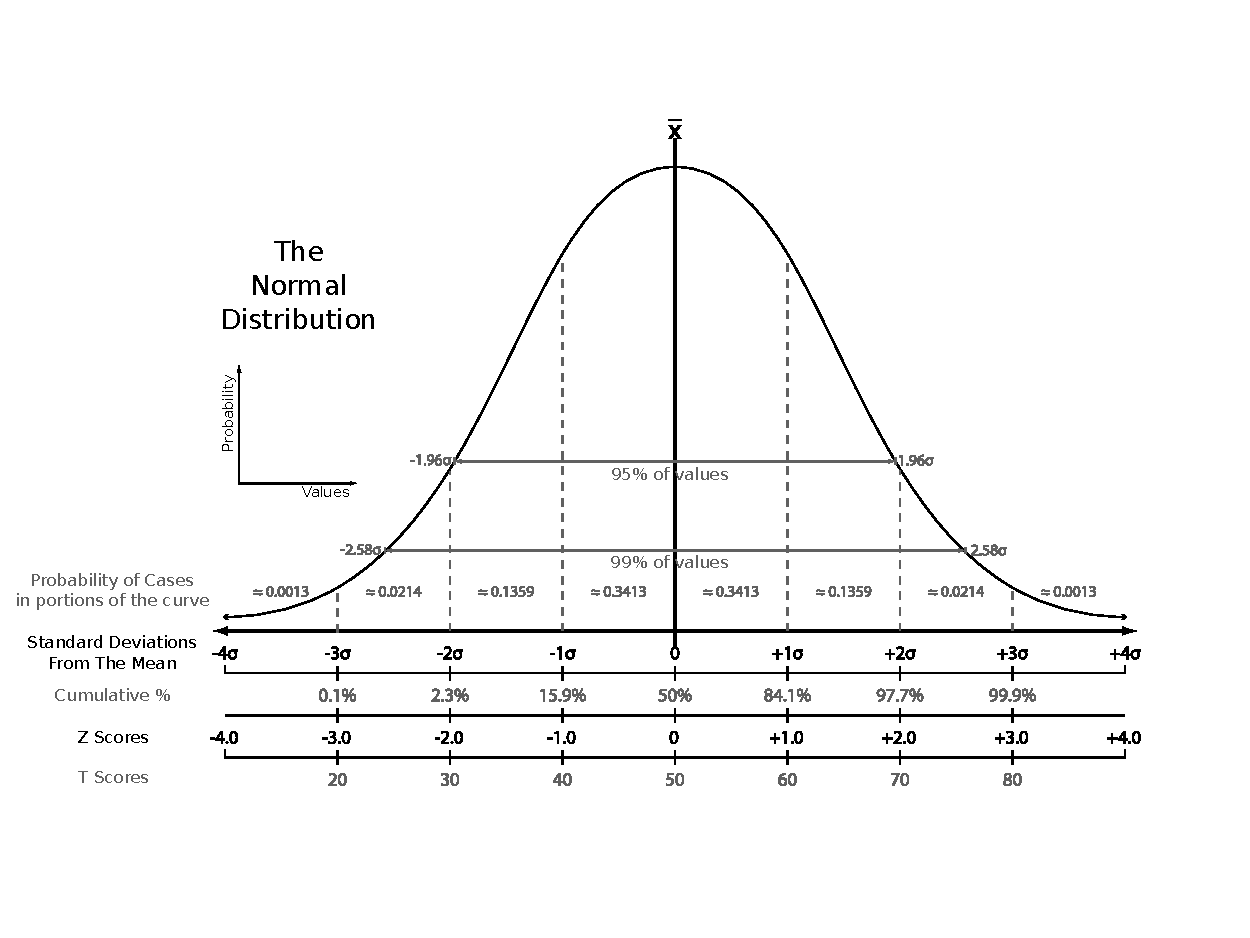
\includegraphics[width=0.8\textwidth]{The_Normal_Distribution.pdf}
	\caption{A~visualization of~the~concept of~standardized value for~a~normal distribution \cite{Wiki:z-score}}\label{fig:z-score}
\end{figure}
%
The mean for~the~U is~calculated by~the~formula
\begin{equation}\label{eq:U-mean}
m_{U} = \frac{n_{1}n_{2}}{2}.
\end{equation}
The~formula for~the standard deviation in~the case of~no~ties is~as~follows:
\begin{equation}\label{eq:standard-deviation-no-ties}
\sigma_{U} =  \sqrt{\frac{n_{1}n_{2}(n_{1}+n_{2}+1)}{12}}.
\end{equation}
In~case of~the~presence of~tied ranks, a~different formula is~used:
\begin{equation}\label{eq:standard-deviation-ties}
\sigma_{U_{ties}} = \sqrt{\frac{n_{1}n_{2}(n_{1}+n_{2}+1)}{12} - \frac{n_{1}n_{2}\sum_{k=1}^{K}({t_{k}}^{3} - t_{k})}{12n(n-1)}} = \sqrt{\frac{n_{1}n_{2}}{12} \left((n+1)-\frac{\sum_{k=1}^{K}({t_{k}}^{3} - t_{k})}{n(n-1)}\right)},
\end{equation}
where~$t_{k}$ is~the~number of~observations with rank~\textit{k} and \textit{K} is~the~total number of~tied ranks. Then, by~obtaining a~standardized value~(z-score) and~using an~approximation of~the~standard normal distribution, the~p-value for~a~given level of~significance (usually~0.05) is~calculated. The~interpretation of~the~result is~as~follows:
\begin{equation}\label{eq:p-interpretation}
\begin{aligned}
p &\leq 0.05 \Rightarrow \text{the~null hypothesis is~rejected}\\
p &> 0.05 \Rightarrow \text{the~null hypothesis can~not~be rejected}.
\end{aligned}
\end{equation}
However, there is~also an~alternative interpretation:
\begin{equation}\label{eq:p-interpretation-2}
\begin{aligned}
p &< 0.05 \Rightarrow \text{the~null hypothesis is~rejected}\\
p &\geq 0.05 \Rightarrow \text{the~null hypothesis can~not~be rejected}.
\end{aligned}
\end{equation}
To~date, there is~no~unambiguous position on~how the~situation when $p = \alpha$ should~be interpreted. This paper uses the~version described in~\ref{eq:p-interpretation}.
%
\section{Relationship to~other statistical tests}
\subsection{Comparison of~Wilcoxon-Mann-Whitney U-test with Student's t-test}
You often hear that the~U-test is~the~nonparametric counterpart of~the~Student's t-test, designed for~data whose distribution differs from the~normal one. From a~purely practical point of~view, we~can indeed say that in~the~case of~a~normal distribution it~is~advisable to~determine whether there is~a~significant difference between the~two samples by~means of~the~t-test, and in~the~case of~a~distribution that differs from the~normal by~means of~the~U-test. Thus, it~can~be said that these tests are~used for~the~same ultimate purpose.

However, the~mathematical meaning of~the~U-test and~the~t-test are~significantly different. As~stated earlier, the~U-test is~designed to~test the~null hypothesis, which is~that for~randomly chosen from two samples of~observations $x \in X$ and~$y \in Y$ the~probability that~\textit{x} is~greater than~\textit{y} is~equal to~the~probability that~\textit{y} is~greater than~\textit{x}, the~alternative hypothesis carries the~claim that these probabilities are~not equal. At~the~same time, the~t-test is~designed to~test the~null hypothesis that the~means of~the~two samples are~equal, while the~alternative hypothesis is~that the~means of~the~two samples are~not~equal. In~this regard, when comparing these tests, we~should keep in~mind that, in~general, the~U-test and~the~t-test check different null hypotheses, although they have partly similar practical meaning. The~result of~the~U-test is~most often very close to~the~result of~the~two-sample t-test for~ranked data. Table~\ref{tab:U-test-t-test-comparison} then provides a~general comparison of~the~U-test with the~t-test.
%
\begin{table}[htp]
	\caption{Properties of~the~U-test relative to~the~t-test.}  \label{tab:U-test-t-test-comparison}
	\centering
	\begin{tabularx}{\textwidth}{p{0.15\linewidth} p{0.8\linewidth}} 
		\hline
		Property&Description\\
		\hline
		Applicability to~ordinal data&When working with ordinal~(rank) data, rather than quantitative data, the~U-test is~preferable to~the~t-test, remembering that the~distance between neighboring values of~the~variation series cannot~be considered constant.\\
		\hline
		Robustness&Since the~U-test handles the~sum of~ranks rather than trait values, it~is less likely than the~t-test to~erroneously indicate significance due~to outliers. However, in~general, the~U-test is~more prone to~type~I error in~the~case when the~data simultaneously have the~property of~heteroscedasticity and~have a~distribution other than normal.\\
		\hline
		Efficiency&In~the~case of~a~normal distribution, the~asymptotic efficiency of~the~U-test is~$\frac{3}{4}\pi \approx 0.95$ of~the~t-test~\cite{U-test-efficiency}. If~the~distribution differs significantly from the~normal one and~the~number of~observations is~large enough, the~efficiency of~the~U-test is~significantly higher than the~efficiency of~the~t-test~\cite{Practical-Nonparametric-Statistics}. However, this efficiency comparison should~be interpreted with caution, because the~U-test and the~t-test examine different hypotheses and~estimate different values. In~the~case, for~example, of~the~need to~compare means, the~use of~the~U-test is~not justified in~principle.\\
		\hline
	\end{tabularx}
\end{table}
%
\subsection{Alternative tests in~the~case of~inequality of~distributions}
If~it~is necessary to~test the~stochastic ordering of~two samples (i.e.~the~alternative hypothesis: $H1:\ P(Y>X)+0.5P(Y=X)\neq0.5$) without assuming equality of~their distributions (i.e.~when the null hypothesis is~$H0:\ P(Y>X)+0.5P(Y=X)=0.5$ but not $F(X)=G(Y)$), more appropriate tests should~be used. These include the~Brunner-Munzel test~\cite{Bruner-Munzel-test-1}, which is~a~heteroskedasticity-resistant analog of~the~U-test, and the~Fligner-Policello test~\cite{Fligner-Policello-test}, which is~a~test for~equality of~medians. In~particular, in~the~case of~a~more general null hypothesis $H0:\ P(Y>X)+0.5P(Y=X)=0.5$, the~U-test can often lead to~a~type~I error even in~the case of~large samples (especially in~the~case of~disparity of~variance and significantly different sample sizes), so~that in~such cases the use of~alternative tests is~preferable~\cite{U-test-vs-Bruner-Munzel-test}. Thus, in~the absence of~the assumption of~equality of~distributions in~case the null hypothesis is~valid, the use of~alternative tests will~be preferable.

In~the case of~testing the hypothesis of~a~shift with significantly different distributions, the U-test may give an~erroneous interpretation of~significance~\cite{U-test-unequal-variance}, so~in~such circumstances it~is preferable to~use a~variant of~the \href{https://en.wikipedia.org/wiki/Welch's_t-test}{t-test}~\cite{Welch-t-test} designed for cases of~unequal variance~\cite{U-test-unequal-variance}. In~some cases, it~may~be justified to~convert quantitative data into ranks and then perform the t-test in~some variant depending on~the assumption of~equality of~variance. When converting quantitative data to~ordinal data, the original variances will not~be preserved; they must~be recalculated for the ranks themselves. In~the case of~equal variance, a~suitable nonparametric substitute for the \href{https://en.wikipedia.org/wiki/F-test}{F-test}~\cite{F-test} can~be the \href{https://en.wikipedia.org/wiki/Brown-Forsythe_test}{Brown-Forsythe test}~\cite{Brown-Forsythe-test}.
%
\subsection{The relationship between the U-test and the classification tasks}\label{U-test&classification}
The U-test is~a particular case of~the \href{https://en.wikipedia.org/wiki/Ordered_logit}{ordered logit model}~\cite{Ordered-logit}.
%
\section{The relationship between the U-test and the concepts of~Receiver operating characteristics~(ROC) and Area under the curve~(AUC)}\label{U-AUC}
Based on~what was said in~\ref{U-test&classification}, we~can conclude that the U-test is~not only a~test for testing the shift hypothesis (or~another one similar in~meaning), but also represents a~kind of~classifier. Looking ahead, the meaning of~the U-test as~a~classifier is~as~follows:
\begin{itemize}
	\item there is~a~"positive" outcome of~comparing two random observations, which is~that the observation from~\textit{X} is~greater than the observation from~\textit{Y};
	\item the proportion of~the sum of~the ranks of~the "positive" elements is~calculated.
	\item as~in~general with ROC, if~the value of~the share of~"positive" elements exceeds~0.5, this means that the classifier generally performs its function; if~it~is equal to~0.5, its efficiency is~equal to~guessing with a~coin flip; if~it~is less than~0.5, using such classifier yields the opposite result.	 
\end{itemize}
At~first glance, the relationship between the U-test and ROC does~not seem obvious. This section will attempt to~understand why these concepts are related and what~is the essence of~the U-test as~a~classifier.

ROC analysis itself is~outside the scope of~this paper. Therefore, let~us consider only its main points.
\begin{description}
	\item[ROC curve ---] is~a~graphical plot that allows us to~evaluate the quality of~binary classification. It~displays the ratio between the proportion of~objects from the total number of~feature carriers correctly classified as~carrying the feature (True Positive Rate~(TPR), called the \emph{sensitivity of the classification algorithm}) and the proportion of~objects from the total number of~objects not carrying the feature, incorrectly classified as~carrying the feature (False Positive Rate~(FPR), the \textbf{1-FPR} value is~called the \emph{specificity of~the classification algorithm}), when varying the threshold of~the deciding rule.	It~is also known as~\textbf{error curve}. Analysis of~classifications using ROC curves is~called \textbf{ROC analysis}.
\end{description}
Quantitative interpretation of~the ROC curve gives the Area under the curve~(AUC).
\begin{description}
	\item[Area under the curve~(AUC) ---] is~the area bounded by~the ROC curve and the axis of~the proportion of~false positive classifications (abscissa axis).
\end{description}
The higher the AUC, the better the quality of~the classifier, while a~value of~0.5 demonstrates the unsuitability of~the chosen classification method (corresponding to~a~random coin guessing). A value of less than 0.5 indicates that the classifier works exactly the other way around: if you call positive results negative and vice versa, the classifier will perform better~\cite{Wiki:ROC}.

Let's introduce some terms.
\begin{description}
	\item[Condition positive~(P) --- ] the number of real positive cases in~the data.
	\item[Condition negative~(N)---] the number of real negative cases in the data.
	\item[True positive~(TP) ---] a~test result that correctly indicates the presence of~a~condition or~characteristic.
	\item[True negative~(TN) ---] a~test result that correctly indicates the absence of~a~condition or~characteristic.
	\item[False positive~(FP) ---] a~test result which wrongly indicates that a~particular condition or~attribute is~present.
	\item[False negative~(FN) ---] a~test result which wrongly indicates that a~particular condition or~attribute is~absent.
\end{description}
Based on~the above, we~can create a~contingency table of~the results of~applying the binary classifier. The rows contain data on~the actual presence or~absence of~the feature, the columns on~the predicted with the classifier.
%
\begin{table}[htp]
	\caption{Binary classifier contingency table.}  \label{tab:ROC-contingency-table}
	\centering
	\begin{tabularx}{\textwidth}{p{0.2\linewidth} p{0.375\linewidth} p{0.375\linewidth}} 
		\hline
	Total $P+N$&Predicted Positive~(PP)&Predicted negative~(PN)\\
		\hline
		Positive~(P)&TP&FN, type~II error~\cite{Wiki:type-1-2-errors}\\
		\hline
		Negative~(N)&FP, type~I error~\cite{Wiki:type-1-2-errors}&TN\\
		\hline
	\end{tabularx}
\end{table}
%
As~can~be seen from Table~\ref{tab:ROC-contingency-table}, the binary classifier can lead to~errors of~two types. Let's introduce some more definitions and define the formulas for calculating the probabilities of~its outcomes~(see tables~\ref{tab:ROC-rates-1}--\ref{tab:ROC-rates-3}).
%
\begin{table}[htp]
	\caption{Additional definitions and formulas for calculating the probabilities of binary classifier outcomes (part~1 of~3).}\label{tab:ROC-rates-1}
	\tiny
	\begin{tabularx}{\textwidth}{p{0.15\linewidth} p{0.4\linewidth} p{0.4\linewidth}} 
		\hline
		Notation&Formula&Deciphering the notation and alternative terms.\\
		\hline
		TPR~(SEN)&\begin{equation}\label{TPR}
		TPR=\frac{TP}{P}=1-FNR=\frac{TP}{TP+FN}
		\end{equation}&\href{https://en.wikipedia.org/wiki/Sensitivity_(test)}{\textbf{true positive rate}}, \href{https://en.wikipedia.org/wiki/Sensitivity_(test)}{\textbf{sensitivity}}~\cite{Wiki:sensitivity-and-specificity}, \href{https://en.wikipedia.org/wiki/Precision_and_recall}{recall}~\cite{Wiki:precision-and-recall}, probability of~detection, \href{https://en.wikipedia.org/wiki/Hit_rate}{hit rate}~\cite{Wiki:hit-rate}, power\\
		\hline
		FPR&\begin{equation}\label{eq:FPR}
		FPR = \frac{FP}{N} = 1 - TNR = \frac{FP}{FP+TN}
		\end{equation}&\href{https://en.wikipedia.org/wiki/False_positive_rate}{\textbf{false positive rate}}, probability of~false alarm, \href{https://en.wikipedia.org/wiki/False_positive_rate}{fall-out}~\cite{Wiki:FPR}\\
		\hline
		FNR&\begin{equation}\label{eq:FNR}
		FNR = \frac{FN}{P} = 1 - TPR = \frac{FN}{FN+TP}
		\end{equation}&\href{https://en.wikipedia.org/wiki/Type_I_and_type_II_errors\#False_positive_and_false_negative_rates}{\textbf{false negative rate}}~\cite{Wiki:TypeI-TypeII-errors}, miss rate\\
		\hline
		TNR~(SPC)&\begin{equation}\label{eq:TNR}
		TNR = \frac{TN}{N} = 1 - FPR = \frac{TN}{TN+FP}
		\end{equation}&\href{https://en.wikipedia.org/wiki/Sensitivity_(test)}{\textbf{true negative rate}}, \href{https://en.wikipedia.org/wiki/Sensitivity_(test)}{\textbf{specificity}}, \href{https://en.wikipedia.org/wiki/Sensitivity_(test)}{selectivity}~\cite{Wiki:sensitivity-and-specificity}\\
		\hline
		PPV&\begin{equation}\label{eq:PPV}
		PPV = \frac{TP}{TP+FP} = 1 - FDR
		\end{equation}&\href{https://en.wikipedia.org/wiki/Positive_and_negative_predictive_values}{\textbf{positive predictive value}}~\cite{Wiki:PPV}, \href{https://en.wikipedia.org/wiki/Information_retrieval\#Precision}{precision}~\cite{Wiki:precision}\\
		\hline
		NPV&\begin{equation}\label{eq:NPV}
		NPV = \frac{TN}{TN+FN} = 1 -FOR
		\end{equation}&\href{https://en.wikipedia.org/wiki/Positive_and_negative_predictive_values}{\textbf{negative predictive value}}~\cite{Wiki:PPV}\\
		\hline
		FDR&\begin{equation}\label{eq:FDR}
		FDR = \frac{FP}{FP + TP} = 1 - PPV
		\end{equation}&\href{https://en.wikipedia.org/wiki/False_discovery_rate}{\textbf{false discovery rate}}~\cite{Wiki:FDR}\\
		\hline
	\end{tabularx}
	\normalsize
\end{table}
%
\begin{table}[htp]
	\caption{Additional definitions and formulas for calculating the probabilities of binary classifier outcomes (part~2 of~3).}\label{tab:ROC-rates-2}
	\tiny
	\begin{tabularx}{\textwidth}{p{0.15\linewidth} p{0.4\linewidth} p{0.4\linewidth}} 
		\hline
		Notation&Formula&Deciphering the notation and alternative terms.\\
		\hline
		FOR&\begin{equation}\label{eq:FOR}
		FOR = \frac{FN}{FN+TN}=1-NPV
		\end{equation}&\href{https://en.wikipedia.org/wiki/Positive_and_negative_predictive_values}{\textbf{false omission rate}}~\cite{Wiki:PPV}\\
		\hline
		LR+&\begin{equation}\label{eq:LR+}
		LR+=\frac{TPR}{FPR}
		\end{equation}&\href{https://en.wikipedia.org/wiki/Likelihood_ratios_in_diagnostic_testing\#positive_likelihood_ratio}{\textbf{\textbf{positive likelihood ratio}}}~\cite{Wiki:likehoods-ratios}\\
		\hline
		LR-&\begin{equation}\label{eq:LR-}
		LR-=\frac{FNR}{TNR}
		\end{equation}&\href{https://en.wikipedia.org/wiki/Likelihood_ratios_in_diagnostic_testing\#negative_likelihood_ratio}{\textbf{negative likelihood ratio}}~\cite{Wiki:likehoods-ratios}\\
		\hline
		PT&\begin{equation}\label{eq:PT}
		PT=\frac{\sqrt{TPR(-TNR+1)}+TNR-1}{TPR+TNR-1}=\frac{\sqrt{FPR}}{\sqrt{TPR}+\sqrt{FPR}}
		\end{equation}&\href{https://en.wikipedia.org/wiki/Sensitivity_(test)}{\textbf{prevalence threshold}}~\cite{Wiki:sensitivity-and-specificity}\\
		TS~(CSI)&\begin{equation}\label{eq:TS|CSI}
		TS = \frac{TP}{TP+TN+FP}
		\end{equation}&\href{https://en.wikipedia.org/wiki/Jaccard_index\#Jaccard_index_in_binary_classification_confusion_matrices}{Jaccard index} \textbf{threat score}, \textbf{critical success index}~\cite{Wiki:jaccard-index}\\
		\hline
		PRV&\begin{equation}\label{eq:PRV}
		PRV = \frac{P}{P+N}
		\end{equation}&\href{https://en.wikipedia.org/wiki/Prevalence}{\textbf{prevalence}}~\cite{Wiki:prevalence}\\
		\hline
		ACC&\begin{equation}\label{eq:ACC}
		ACC = \frac{TP+TN}{P+N} = \frac{TP+TN}{TP+TN+FP+FN}
		\end{equation}&\href{https://en.wikipedia.org/wiki/Accuracy_and_precision}{\textbf{accuracy}}~\cite{Wiki:accuracy-precision}\\
		\hline
	\end{tabularx}
	\normalsize
\end{table}
%
\begin{table}[htp]
	\caption{Additional definitions and formulas for calculating the probabilities of binary classifier outcomes (part~3 of~3).}\label{tab:ROC-rates-3}
	\tiny
	\begin{tabularx}{\textwidth}{p{0.15\linewidth} p{0.4\linewidth} p{0.4\linewidth}} 
		\hline
		Notation&Formula&Deciphering the notation and alternative terms.\\
		\hline
		BA&\begin{equation}\label{eq:BA}
		BA = \frac{TPR+TNR}{2}
		\end{equation}&\textbf{balanced accuracy}\\
		\hline
		F1 score&\begin{equation}\label{eq:F1-score}
		F_{1} = 2 \times \frac{PPV \times TPR}{PPV +TPR} = \frac{2TP}{2TP + FP + FN}
		\end{equation}&\href{https://en.wikipedia.org/wiki/F-score}{F1 score} is~the harmonic mean of~\href{https://en.wikipedia.org/wiki/Information_retrieval\#Precision}{precision} and \href{https://en.wikipedia.org/wiki/Sensitivity_(test)}{sensitivity}~\cite{Wiki:F-score}\\
		\hline
		MCC~($\phi$ or~$r_{\phi}$)&\begin{equation}\label{eq:MCC}
		MCC = \frac{TP \times TN - FP \times FN}{\sqrt{(TP+FP)(TP+FN)(TN+FP)(TN+FN)}}
		\end{equation}&\href{https://en.wikipedia.org/wiki/Phi_coefficient}{\textbf{Matthews correlation coefficient}},\href{https://en.wikipedia.org/wiki/Phi_coefficient}{\textbf{phi coefficient}}~\cite{Wiki:phi-coefficient}\\
		\hline
		FM&\begin{equation}\label{eq:FM}
		FM = \sqrt{\dfrac{TP}{TP+FP} \times \dfrac{TP}{TP+FN}} = \sqrt{PPV \times TPR}
		\end{equation}&\href{https://en.wikipedia.org/wiki/Fowlkes–Mallows_index}{Fowlkes–Mallows index}~\cite{Wiki:Fowlkes–Mallows-index}\\
		\hline
		BM&\begin{equation}\label{eq:BM}
		BM = TPR + TNR -1
		\end{equation}&\textbf{bookmaker informedness}, \href{https://en.wikipedia.org/wiki/Youden's_J_statistic}{informedness}~\cite{Wiki:j-statistic}\\
		\hline
		MK~($\delta P$)&\begin{equation}\label{eq:MK}
		MK = PPV + NPV - 1
		\end{equation}&\href{https://en.wikipedia.org/wiki/Markedness}{\textbf{markedness}}, deltaP~\cite{Wiki:markedness}\\
		\hline
		DOR&\begin{equation}\label{eq:DOR}
		\frac{LR+}{LR-}
		\end{equation}&\href{https://en.wikipedia.org/wiki/Diagnostic_odds_ratio}{\textbf{diagnostic odds ration}}~\cite{Wiki:DOR}\\
		\hline
	\end{tabularx}
	\normalsize
\end{table}
%
The TPR probability can~be written as
\begin{equation}\label{eq:TPR-probability}
P_{TPR} = \mathbb{P}(1,\ x\in C_{1}),
\end{equation}
which means that if~object~\textit{x} belongs to~class~$C_{1}$, this indicator estimates the probability that the binary classifier assigns object~\textit{x} to~this class. The probability of~FPR is~written as
\begin{equation}\label{eq:FPR-probability}
P_{FPR} = \mathbb{P}(1,\ x\in C_{0}),
\end{equation}
which means the probability that an~object belonging to class~$C_0$ will~be mistakenly assigned to~class~$C_1$.

Typically, the working principle of~a~binary classifier is~based on~comparing the measurement of~\textit{x} with some fixed threshold~\textit{c}. It~follows that the previous two expressions can~be rewritten and combined into a~system.
\begin{equation}\label{eq:TRP+FPR-probability}
\begin{cases}
P_{TPR} = \mathbb{P}(x>c,\ x \in C_{1})\\
P_{FPR} = \mathbb{P}(x>c,\ x \in C_{0})
\end{cases}
\end{equation}
It~follows that the ROC curve is~a~diagram
\begin{equation}\label{eq:ROC-contour}
P_{FPR}(c),\ P_{TPR}(c),
\end{equation}
thus, drawing the curve means changing the value of~threshold~\textit{c}.

Let's consider the example~\cite{AUC-Derivation}. Let's take~$f(x\in C_{0}) = \mathcal{N}(0,1)$ and~$f(x\in C_{1}) = \mathcal{N}(2,1)$ as~probability density functions~$C_{0}$ and~$C_{1}$, respectively. Next we~build the ROC curve step by~step using the Python language. At~the first step, consider diagram~\ref{fig:plot-TPR-FPR-prob-density-1}, built using the code given in~script~\ref{lst:plot-TPR-FPR-prob-density}. The area shaded blue shows the probability of~FPR, i.\,e., false-positive significance detection, while the area shaded green shows the probability density of TPR, i.\,e., correct significance detection. The ROC curve shows the values of~these very indicators. The vertical dashed line is~the sensitivity threshold~\textit{c}. In~this situation it~is at~0 on~the abscissa axis. If~it~is moved to~1, the area under the FPR curve (blue) will significantly decrease, i.\,e. the probability of~false-positive detection will decrease, but the TPR area (green) will decrease as~well, which means an~increase in~the probability of~false-negative results. This situation is~illustrated in~Diagram~\ref{fig:plot-TPR-FPR-prob-density-2}.
%
\begin{figure}[htp]
	\centering
	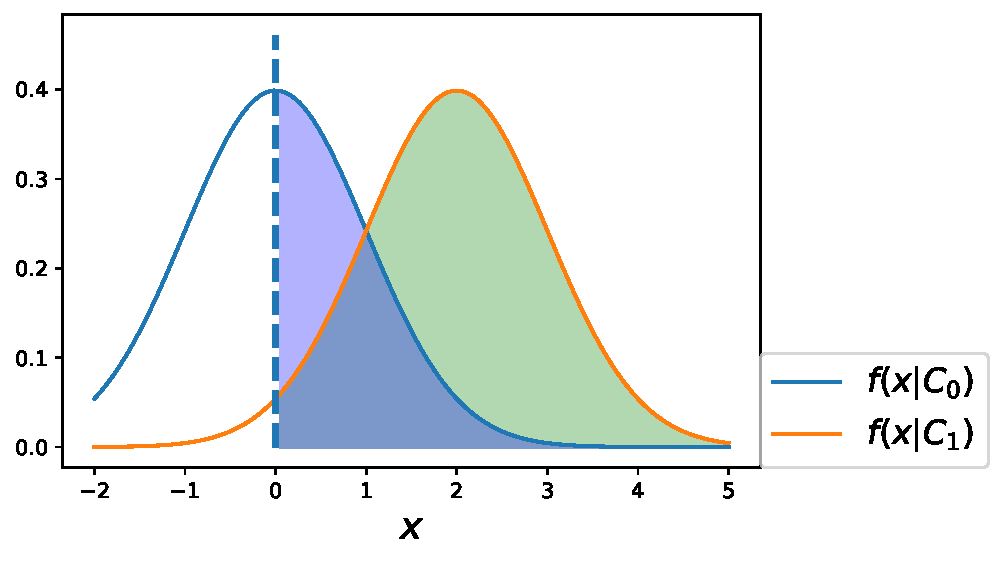
\includegraphics[width=0.95\textwidth]{Plot-ROC-step-1.pdf}
	\caption{Diagram of~TPR and FPR probability distribution densities at~threshold~0.}
	\label{fig:plot-TPR-FPR-prob-density-1}
\end{figure}
%
\begin{lstlisting}[float=htp, caption = Plotting TPR and FPR probability density functions, firstnumber=1, label= lst:plot-TPR-FPR-prob-density]
# Import Libraries
import numpy as np
import matplotlib.pyplot as plt
from scipy import stats

# Plot
f0 = stats.norm(0, 1)
f1 = stats.norm(2, 1)
fig, ax = plt.subplots()
xi = np.linspace(-2, 5, 100)
ax.plot(xi, f0.pdf(xi), label=r'$f(x|C_0)$')
ax.plot(xi, f1.pdf(xi), label=r'$f(x|C_1)$')
ax.legend(fontsize=16, loc=(1, 0))
ax.set_xlabel(r'$x$', fontsize=18)
ax.vlines(0, 0, ax.axis()[-1] * 1.1, linestyles='--', lw=3.)
ax.fill_between(xi, f1.pdf(xi), where=xi > 0, alpha=.3, color='g')
ax.fill_between(xi, f0.pdf(xi), where=xi > 0, alpha=.3, color='b')

# Save to .pdf
plt.savefig('Plot-ROC-step-1.pdf', bbox_inches='tight')

\end{lstlisting}
%
\begin{figure}[htp]
	\centering
	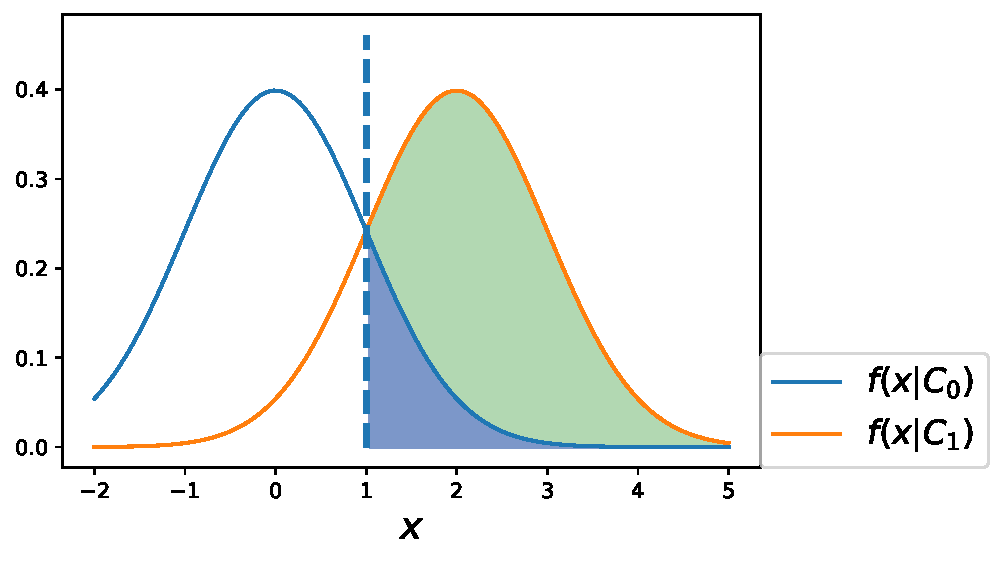
\includegraphics[width=0.95\textwidth]{Plot-ROC-step-2.pdf}
	\caption{Diagram of~TPR and FPR probability distribution densities at~threshold~1.}
	\label{fig:plot-TPR-FPR-prob-density-2}
\end{figure}

As~you can see from the diagrams above, increasing the threshold leads to~the loss of~a~part of~both true-positive and false-positive results, while decreasing~it leads to~an~increase in~the number of~fixations of~the feature presence (both true and false). In~extreme cases, too low a~threshold value will lead to~the fact that all results will~be interpreted as~positive, too high --- to~a~zero number of~observations in~which the feature was detected. The task of~ROC analysis is~to~choose a~rational threshold value.

Let's add the ROC curves corresponding to~thresholds~0 and~1 to~the already existing diagrams. And also create an~interactive diagram using the code from script~\ref{lst:plot-TPR-FPR-prob-density+ROC-interactive}. The PDF format does~not allow you to~add such interactive elements, so~let's consider cases with fixed values of~0 and~1, shown in~Diagrams~\ref{fig:plot-TPR-FPR-prob-density-3} and \ref{fig:plot-TPR-FPR-prob-density-4}, respectively. The left side of~each of~them shows the already familiar probability density function graphs for the TPR and FPR distributions. The right part shows the ROC curve and the point corresponding to~the set threshold value. It~is easy to~guess that the x-coordinate of~the point matches the area under the FPR curve, and the y-coordinate matches the area under the TPR curve. Increasing the threshold value entails shifting the point to~the left, decreasing~it to~the right.

The better the binary classifier itself, the closer to~the upper left corner will~be the ROC curve corresponding to~it, because in~this case a~high TPR value will~be combined with a~low FPR value. The binary classifier, which works as~well (actually badly) as~the coin flip guessing algorithm (in~case the coin is~"fair"), gives a~ROC curve, which is~a~straight line between~(0,0) and~(1,1). In~this case, the left part of~the diagram will show a~complete overlap of~TPR and FPR probability density function curves. Such a~case is~shown in~Diagram~\ref{fig:plot-TPR-FPR-prob-density-3}. For self-practice, you can use Script~\ref{lst:plot-TPR-FPR-prob-density+ROC-interactive} by~running~it in~the Jupyter Lab environment, which allows you to~use the interactive features of~the browser.
%
\begin{lstlisting}[float=htp, caption = Build an~interactive graph of~TPR and FPR distribution density and its corresponding ROC curve for a~given threshold value, firstnumber=1, label= lst:plot-TPR-FPR-prob-density+ROC-interactive]
# Import Libraries
%matplotlib inline
from ipywidgets import interact
import numpy as np
import matplotlib.pyplot as plt
from scipy import stats

# Plot
f0 = stats.norm(0, 1)
f1 = stats.norm(2, 1)
fig, ax = plt.subplots()
xi = np.linspace(-2, 5, 100)
ax.plot(xi, f0.pdf(xi), label=r'$f(x|C_0)$')
ax.plot(xi, f1.pdf(xi), label=r'$f(x|C_1)$')
ax.legend(fontsize=16, loc=(1, 0))
ax.set_xlabel(r'$x$', fontsize=18)
ax.vlines(0, 0, ax.axis()[-1] * 1.1, linestyles='--', lw=3.)
ax.fill_between(xi, f1.pdf(xi), where=xi > 0, alpha=.3, color='g')
ax.fill_between(xi, f0.pdf(xi), where=xi > 0, alpha=.3, color='b')

# Plot ROC-curve and make all interactive
def plot_roc_interact(c=0):
xi = np.linspace(-3,5,100)
fig,axs = plt.subplots(1,2)
fig.set_size_inches((10,3))
ax = axs[0]
ax.plot(xi,f0.pdf(xi),label=r'$f(x|C_0)$')
ax.plot(xi,f1.pdf(xi),label=r'$f(x|C_1)$')
ax.set_xlabel(r'$x$',fontsize=18)
ax.vlines(c,0,ax.axis()[-1]*1.1,linestyles='--',lw=3.)
ax.fill_between(xi,f1.pdf(xi),where=xi>c,alpha=.3,color='g')
ax.fill_between(xi,f0.pdf(xi),where=xi>c,alpha=.3,color='b')
ax.axis(xmin=-3,xmax=5)
crange = np.linspace(-3,5,50)
ax=axs[1]
ax.plot(1-f0.cdf(crange),1-f1.cdf(crange))
ax.plot(1-f0.cdf(c),1-f1.cdf(c),'o',ms=15.)
ax.set_xlabel('False-alarm probability')
ax.set_ylabel('Detection probability')

interact(plot_roc_interact,c=(-3,5,.05))

\end{lstlisting}
%
\begin{figure}[htp]
	\centering
	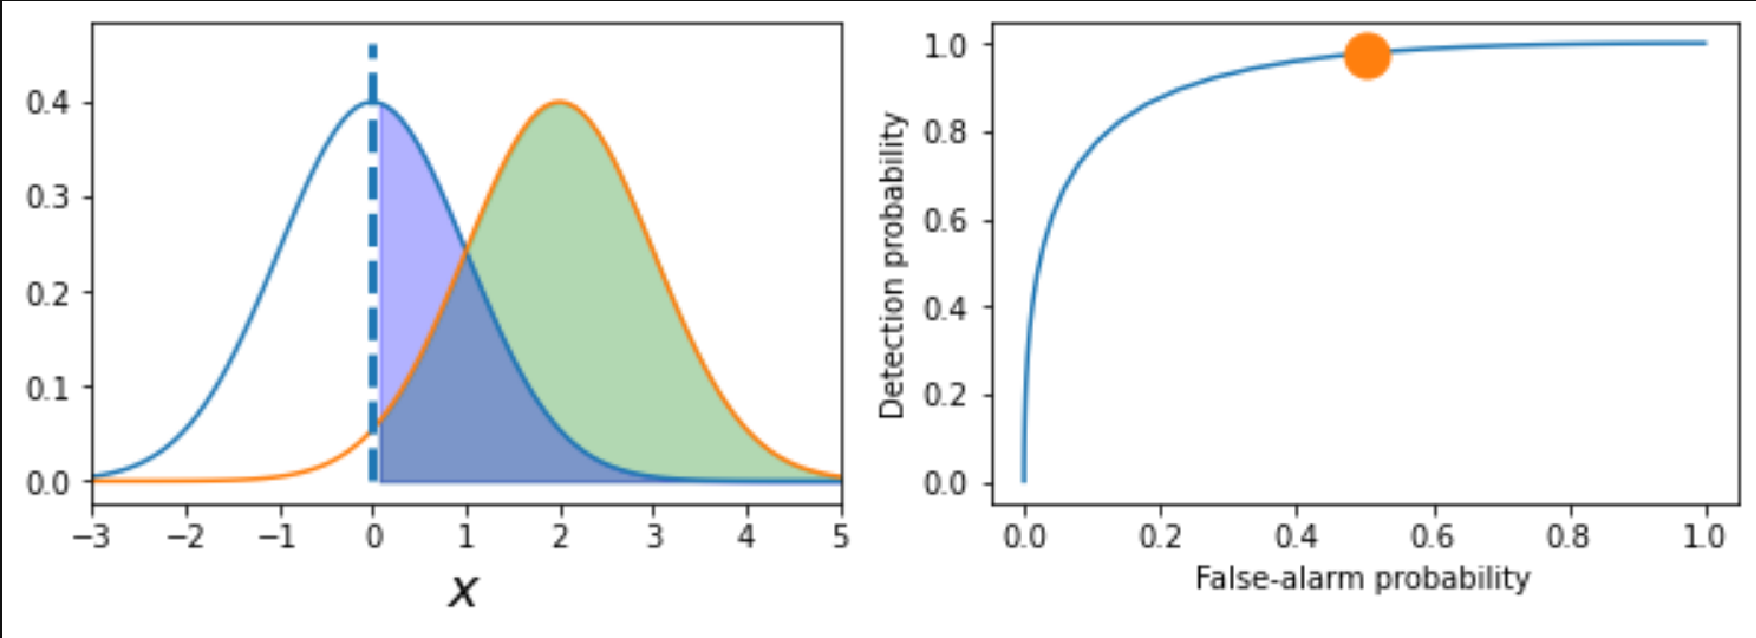
\includegraphics[width=0.95\textwidth]{Plot-ROC-step-30.pdf}
	\caption{Diagram of~TPR and FPR probability distribution densities at~threshold~0.}
	\label{fig:plot-TPR-FPR-prob-density-3}
\end{figure}
%
\begin{figure}[htp]
	\centering
	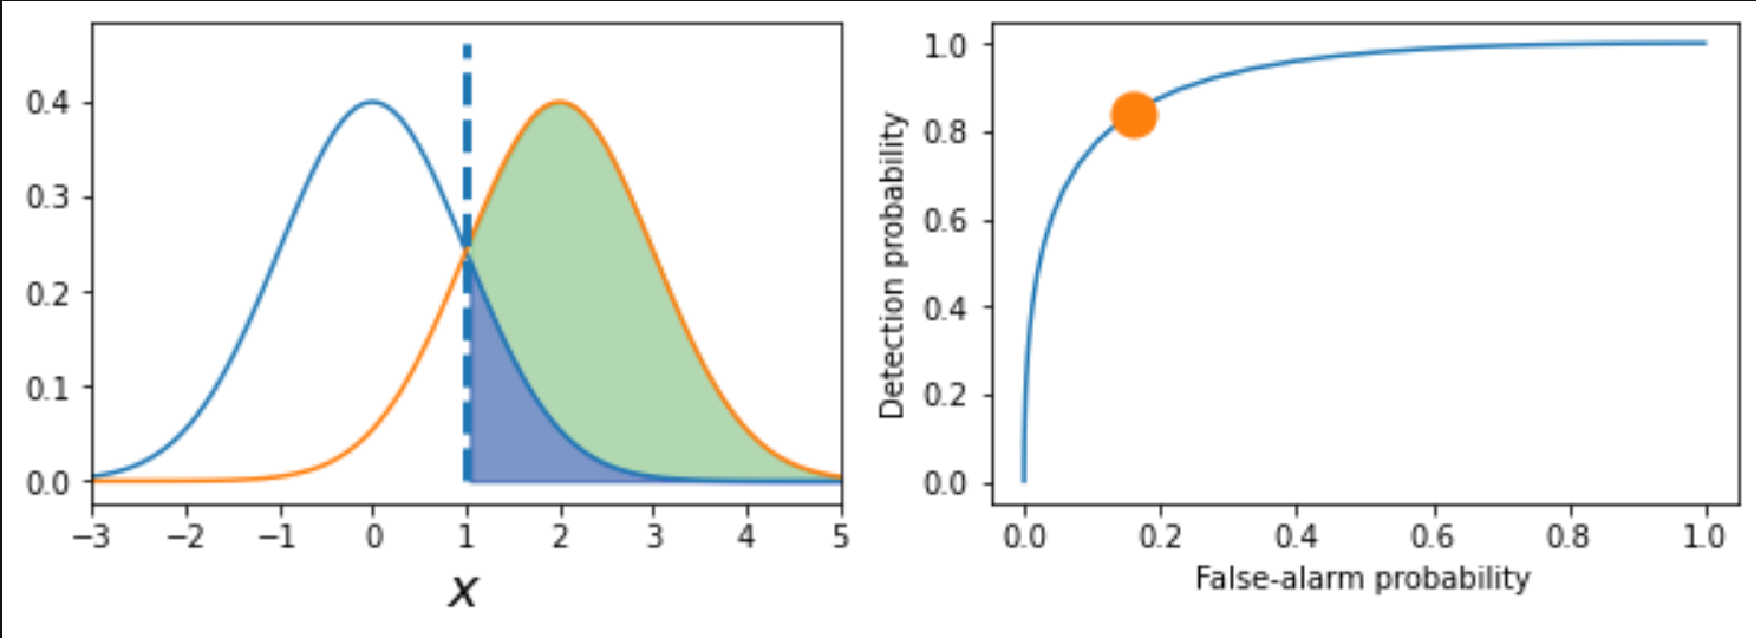
\includegraphics[width=0.95\textwidth]{Plot-ROC-step-4.pdf}
	\caption{Diagram of TPR and FPR probability distribution densities at threshold 1.}
	\label{fig:plot-TPR-FPR-prob-density-4}
\end{figure}
%
\begin{figure}[htp]
	\centering
	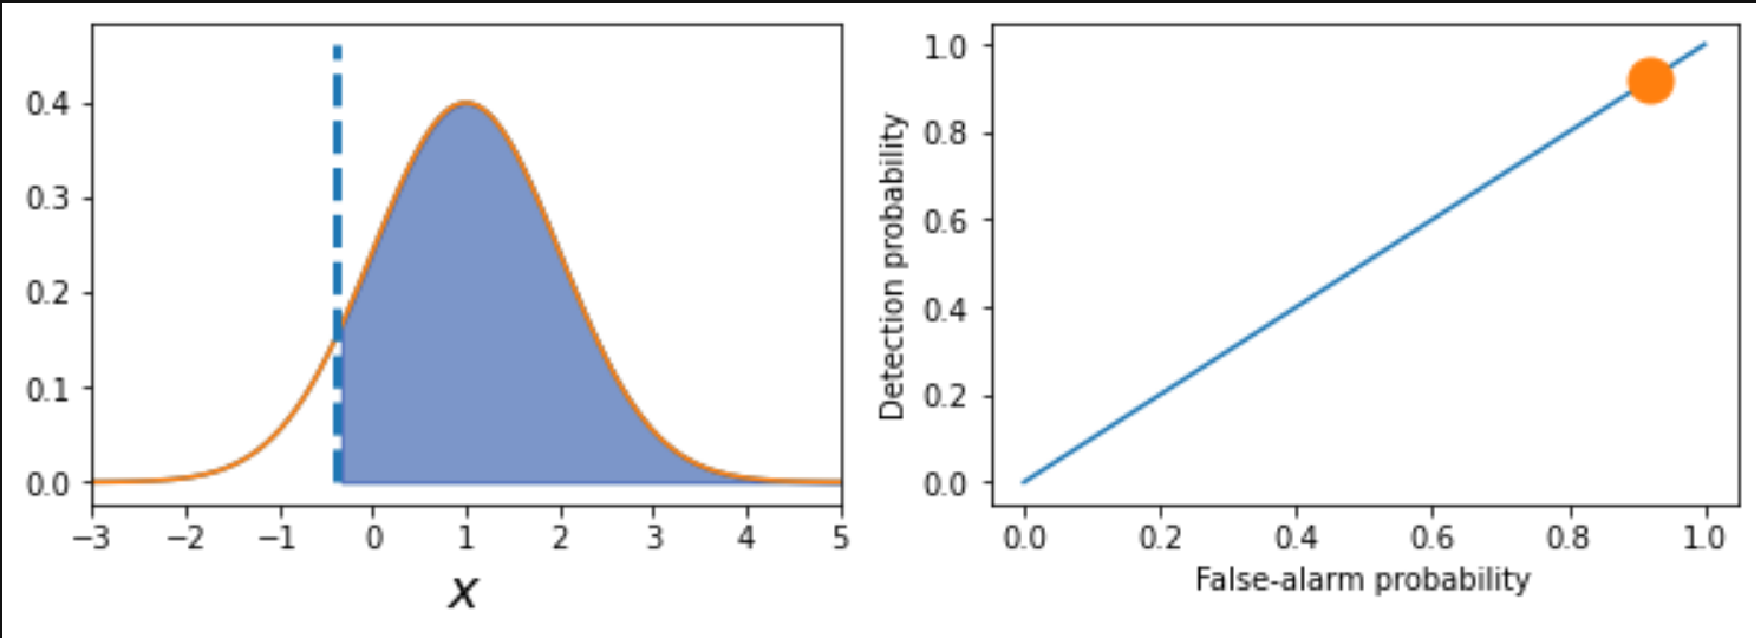
\includegraphics[width=0.95\textwidth]{Plot-ROC-step-5.pdf}
	\caption{Diagram of~probability densities of~TPR and FPR probability distributions at~equal mean.}
	\label{fig:plot-TPR-FPR-prob-density-5}
\end{figure}
%
\subsection{The concept of~AUC and its calculation}
As~the name implies, the AUC is~the area under the ROC curve bounded by~the point corresponding to~a~given threshold value. In~the normalized space in~which the ROC curve is~usually plotted, the AUC value is~equivalent to~the probability that the classifier assigns a~higher weight to~a~randomly chosen positive entity than to~a~randomly chosen negative entity. The AUC does not depend on~a~specific threshold value, because the ROC curve is~constructed by~fitting~it. This means that the AUC is~calculated by~integrating over the thresholds. The AUC is~given by~the expression:
\begin{equation}\label{eq:AUC-computation-0}
AUC = \int P_{TPR}(P_{FPR}) d P_{FPR}.
\end{equation}
The step-by-step calculation of~the AUC is~as~follows.
\begin{equation}\label{eq:AUC-computation-1}
P_{TPR}(c) = 1 - F_{1}(c),
\end{equation}
where~$F_{1}$ is~the cumulative density function for~$C_{1}$. Similarly calculate
\begin{equation}\label{eq:AUC-computation-2}
P_{FPR}(c) = 1 - F_{0}(c),
\end{equation}
where~$F_{0}$ is~the cumulative density function for~$C_{0}$.


Let~us take some particular value of~$c^{*}$ to~which a~certain~$P_{FPR}(c^{*})$ corresponds. In~other words, it~corresponds to~the probability that a~random element~$x_{0}$ belonging to~class~$C_{0}$ is~greater than the threshold value~$c^{*}$, i.e.
\begin{equation}\label{eq:AUC-computation-3}
P_{FPR}(c^{*}) = \mathbb{P}(x_{0}>c^{*}|x_{0} \in C_{0}).
\end{equation}
Then, reasoning similarly with respect to~TPR, we~get
\begin{equation}\label{eq:AUC-computation-4}
P_{TPR}(c^{*}) = \mathbb{P}(x_{1}>c^{*}|x_{1} \in C_{1}).
\end{equation}
Next, based on~the fact that the AUC is~realized through an~integral, we~select its value so~that the distribution of~$c^{*}$ matches the distribution of~$F_{0}$. In~this case,~$P_{TPR}$ is~an~independent random variable with a~corresponding expectation in~the form of
\begin{equation}\label{eq:AUC-computation-integral}
\mathbb{E}(P_{TPR}) = \int P_{TPR} d P_{FPR} = AUC.
\end{equation}
It~is~now possible to~formulate a~definition for the AUC.
\begin{description}
	\item[AUC ---] is~the expected probability that element~$x_{1} \in C_{1}$ will~be assigned to~$C_{1}$ with higher probability than element~$x_{0} \in C_{0}$. Thus,
	\begin{equation}\label{eq:AUC-definition}
	1-F_{1}(t)>1-F_{0}(t) \forall t.
	\end{equation}
	The wording "for any t" means that~$1-F_{1}(t)$ is~\emph{stochastically} greater than~$1-F_{0}(t)$. The latter circumstance is~key in~terms of~the relationship of~the AUC to~the U-test, which will~be shown later.
\end{description}
%
\subsection{Relation between U-test and AUC}\label{U-test&AUC-relation}
A~fairly detailed description of~the U-test was given earlier. This subsection contains only brief information about~it, which is~directly relevant to~the question of~its relationship to~the AUC.

The U-test is~a~non-parametric test that allows you to~test whether two samples belong to~the same distribution. His basic idea is~that if~there is~no~difference between two classes, then combining them into one larger class (set) and then calculating any statistic for the new larger class will give an~unbiased estimate for any of~the initial classes. In~other words, if~there is~no~difference in~the distribution of~the two samples, combining them and assuming that the actually observed data from the two samples represent only one of~the equal-valued variants of~the moving observations means that there is~no~difference in~any statistical estimate for any of~the moving variants relative to~the other, and relative to~the combined set.

Let's suppose that we~need to~compare two samples using the median, the mean, or~some other measure of~central tendency. In~terms of~cumulative distribution functions for the two populations, in~the case of~$H0$ we~have the following:
\begin{equation}\label{eq:U-AUC-H0}
H_0: F_{X}(t) = F_{Y}(t), \quad \forall t,
\end{equation}
which indicates that all observations belong to~the same distribution. Then an~alternative hypothesis is~that
\begin{equation}\label{eq:U-AUC-H1}
H_1: F_{X}(t) < F_{Y}(t), \quad \forall t,
\end{equation}
which is~possible, in~particular, in~the case of~the existence of~a~shift of~one distribution relative to~the other. In~this case, the samples ${X_{i}}_{i=1}^{n},\ {X_{j}}_{j=1}^{m}$ represent independent groups of~observations. In~this case, the size of~the samples may vary.

The test technique consists of~combining two samples into one set and assigning ranks to~each item within~it. The U-statistic is~the sum of~the ranks for the set~\textit{X}. If~the value of~the statistic is~small enough, it~means that the distribution of~set~\textit{X} is~stochastically shifted to~the left relative to~the distribution of~set~\textit{Y}, i.\,e.~$F_{X}{t} < F_{Y}{t}$.

Since with a~sufficiently large number of~observations (20 or~more) the distribution of~U-statistics is~well approximated by~the normal distribution, the p-value is~suitable for assessing significance. Let's calculate it~using the Python language according to~the script~\ref{lst:AUC-p-value}.
%
\begin{lstlisting}[float=htp, caption = Calculation of~the p-value for the test data, firstnumber=1, label= lst:AUC-p-value]
print('p-value:',stats.wilcoxon(f1.rvs(30), f0.rvs(30))[1])

\end{lstlisting}
The p-value is~1.9729484515803686e-05, which is~less than the significance level~(0.05), so~we~can reject the null hypothesis~\ref{eq:U-AUC-H0}. Since the data were randomly generated, if~the experiment is~repeated, the particular p-value will differ from that obtained when writing this paper. However, it~will always be below the threshold because of~the parameters set in~the algorithm.

The U-statistic can be~written as~follows:
\begin{equation}\label{eq:U-statistics}
U = \frac{1}{mn}\sum_{i=1}^{m}\sum_{j=1}^{n}\mathbbm{1}{(Y_{j}>X_{i})},
\end{equation}
where~$\mathbbm{1}{(Y_{j}>X_{i})}$ is~the indicator (characteristic) function showing that the statistic (for the discrete case) estimates the probability that~\textit{Y} is~stochastically greater than~\textit{X}. Thus, this correspondence means that its value is~equal to~the AUC. The relationship between the AUC and the U-test is~in a~similar sense: checking the stochastic excess value of~observations belonging to~one sample relative to~observations belonging to~another sample.
%
\subsection{Practice of~ROC analysis and AUC calculation.}\label{ROC-AUC-theory}
This subsection is~not required reading if~the goal is~only the practical implementation of~the U-test itself. However, it~gives an~insight into machine learning methods that are not related to~the so-called \emph{frequentist statistics} to~which the U-test itself belongs, and shows the relationship between these areas of~data analysis. In~addition, it~will provide sufficient knowledge to~perform a~ROC analysis as~such, which may~be useful in~other situations that an~appraiser may encounter in~his or~her practice.
%
\subsubsection{Plotting the ROC curve}\label{plot-ROC-theory}
%
\lstset{language=R,
	basicstyle=\ttfamily,
	keywordstyle=\color{Blue}\ttfamily,
	stringstyle=\color{Red}\ttfamily,
	commentstyle=\color{Emerald}\ttfamily,
	morecomment=[l][\color{Magenta}]{\#},
	breaklines=true,
	breakindent=0pt,
	breakatwhitespace,
	columns=fullflexible,
	showstringspaces=false
}
%
ROC analysis and in~particular the construction of~ROC curves are widely used to~find a~compromise between the \emph{sensitivity} and \emph{specificity} of~a~binary classifier. Most of~the classifiers used in~machine learning produce a~result in~the form of~a~quantification that a~given object has a~"positive" feature value. Some threshold value is~needed to~convert such a~quantitative assessment into a~concrete "yes" or~"no" prediction. In~his case, observations with a~score above this threshold will~be classified as~"positive", below as~"negative". Different thresholds provide different levels of~sensitivity and specificity. Setting a~relatively high threshold value provides a~conservative approach to~the issue of~classifying a~particular case as "positive", which reduces the likelihood of~false positives. At~the same time, this increases the risk of~missing the observed positive values, i.\,e., it~reduces the level of~true positive classification results. A~relatively low threshold value provides a~more liberal approach to~classifying observations as~"positive".  This reduces specificity (increases the number of~false negatives) and increases sensitivity (increases the number of~true positives). The ROC curve shows the ratio of~true positives to~false positives, giving an~overview of~the entire spectrum of~such trade-offs. There are many R~language libraries that plot ROC curves and calculate metrics for ROC analysis. In~this case, to~better understand the essence of~ROC analysis, some actions will~be performed by~writing our own functions. The following will show an~algorithm for constructing a~ROC curve based on~a~set of~real outcomes and their corresponding estimates. The calculation involves two steps:
\begin{itemize}
	\item sort the observed outcomes in~descending order by~their predicted scores;
	\item calculation of~total true positive (TPR) and true negative (TNR) scores for ordered observed outcomes.
\end{itemize}
Let's create an appropriate function (script~\ref{lst:create-ROC-function-R}).
%
\begin{lstlisting}[float=htp, caption = Creating a~function to~calculate TPR and FPR, firstnumber=1, label= lst:create-ROC-function-R]
# create own function for ROC
appraiserRoc <- function(labels, scores){
labels <- labels[order(scores, decreasing=TRUE)]
data.frame(TPR=cumsum(labels)/sum(labels),
FPR=cumsum(!labels)/sum(!labels), labels)
}
 
\end{lstlisting}
%
This function has two inputs:
\begin{itemize}
	\item \emph{labels} --- Boolean vector containing actual classification data;
	\item \emph{scores} --- a~vector of~real numbers containing data about the scores predicted by~some classifier.
\end{itemize}
%
Since only two classification outcomes are possible, the labels vector can only contain \emph{TRUE} or~\emph{FALSE} values (or~\emph{1} and~\emph{0} depending on~the analyst's preference). A~sequence of~such binary values can~be interpreted as~a~set of~instructions for a~\href{https://en.wikipedia.org/wiki/Turtle_graphics}{turtle graphics}~\cite{Wiki:turtle-graphics}. There~is one important feature: in~this case the turtle has a~compass and receives instructions for absolute directions of~movement: "to~the north" or~"to~the east" instead of~relative "to~the right" and "to~the left". The turtle starts its movement from the starting point with coordinates~(0,0) and makes its way on~the plane according to~the sequence of~instructions. When a~\emph{TRUE} command is~received, it~takes one step north, i.\,e., in~the positive direction of~the y-axis, and when a~\emph{FALSE} command is~received, it~takes one step east, i.\,e., in~the positive direction of~the x-axis. The length of~the steps is~chosen in~such a~way that if~all \emph{TRUE~(1)} commands are received consecutively, the turtle will~be at~a~point with coordinates~(0,1), all \emph{FALSE~(0)} commands at~a~point with coordinates~(1,0). Thus, the length of~the step "to~the north" may~be different from the length of~the step "to~the east". The path in~the plane is~determined by~the order of~the \emph{TRUE~(1)} and \emph{FALSE~(0)} commands and always ends at~(1,1).

Advancing the turtle through the bits of~the instruction string is~an~adjustment of~the classification threshold to~less and less stringent. Once the turtle has passed the bit, it~means that it~has decided to~classify that bit as~"positive". If~this bit was actually "positive", it~is a~true positive, if~it~was actually "negative" it~is a~false positive. The y-axis shows the TPR, calculated as~the ratio of~the number of~positive results detected to~this time to~the total number of~actual positive results. The x-axis shows the (FPR), calculated as~the ratio of~the number of~currently detected positive results to~the total number of~actual negative results. The vectorized implementation of~this logic uses cumulative sums (the \textbf{cumsum} function) instead of~going through the values one by~one, although that is~what the computer does at~a~lower level.

The ROC curve calculated in~this way is~actually a~step function. With a~very large number of~positive and negative cases, these steps are very small, and the curve looks smooth. In~this case, with a~really large number of~observations, the construction of~each point is~difficult. As~a~consequence, in~practice, most ROC curve functions used for practical purposes contain additional steps and often use some form of~approximation.

As~an~example, consider a~situation in~which an~appraiser evaluates parts manufactured by~an~enterprise. Some of~the parts are known to~be of~good quality and some are defective. The valuation of~quality parts is~carried out on~the basis of~cost market approaches in~the usual manner. And defective parts are valued at~a~scrap value. In~this case, it~is necessary to~assign each part to~one or~another category. There is~some feature~\emph{x}, which can~be measured by~the appraiser. And there is~also some feature~\emph{y}, which cannot~be measured by~the appraiser. The value of~the feature~\emph{y} allows you to~classify parts as~quality or~defective. It~is also known that there is~some finitary relation function between features \emph{x} and~\emph{y}. Thus, knowing the value of~\emph{x}, we~can infer the value of~y with some probability.
In~this case, it~is advisable to~take a~certain sample of~parts. Then, together with the specialists of~the customer company, measure the values of~features \emph{0} and~\emph{y} for each element of~this sample.

We~will use simulated data to~consider the example. There is~some input feature~\emph{x} that is~linearly related to~the implicit result~\emph{y}. This relationship implies the presence of~some randomness. The y-value shows whether the part exceeds the tolerance requirements. If~so, it~should~be classified as~defective. The algorithm used in~this paper involves the following steps:
\begin{itemize}
	\item create the~\textbf{sim\_parts\_data} function that generates data according to~certain rules and sets the $"y>100"$ threshold value to~classify parts as~defective.
	\item create the~dataframe \textbf{parts\_data} with this function;
	\item create the~\textbf{test\_set\_idx} rule, whereby 80\,\% of~the data is~randomly assigned to~the training sample, and 20\,\% to the test sample;
	\item applying the rule \textbf{test\_set\_idx} to~data \textbf{parts\_data};
	\item create training (\textbf{<<training\_set>>}) and testing (\textbf{<<test\_set>>}) sub-samples;
	\item plot the diagram showing the distribution of~observations from the training sample.
\end{itemize}
To~implement the above algorithm, the code from script~\ref{lst:create-sample-data-plot-graph-R} was used.
%
\begin{lstlisting}[float=htp, caption = Creation and primary visualization of~data on~quality and defective parts, firstnumber=1, label= lst:create-sample-data-plot-graph-R]
# Sample of ROC-analysis

# enable libraries
library(ggplot2)
library(dplyr)
library(pROC)

#set seed
set.seed(19190709)

# create own function for ROC
appraiserRoc <- function(labels, scores){
labels <- labels[order(scores, decreasing=TRUE)]
data.frame(TPR=cumsum(labels)/sum(labels),
FPR=cumsum(!labels)/sum(!labels), labels)
}

# create function 
sim_parts_data <- function(N, noise=100){
x <- runif(N, min=0, max=100)
y <- 122 - x/2 + rnorm(N, sd=noise)
bad_parts <- factor(y > 100)
data.frame(x, y, bad_parts)
}

# create dataset
parts_data <- sim_parts_data(2000, 10)

# create rule for test subset
test_set_idx <- sample(1:nrow(parts_data), size=floor(nrow(parts_data)/4))

# create training and test subsets
test_set <- parts_data[test_set_idx,]
training_set <- parts_data[-test_set_idx,]

# plot graph
test_set %>% 
ggplot(aes(x=x, y=y, col=bad_parts)) + 
scale_color_manual(values=c("green", "red")) + 
geom_point() + 
ggtitle("Bad parts related to x")

\end{lstlisting}
%

The result was diagram~\ref{fig:bad-parts-r}. As~you can see, if~the value of~the parameter~\emph{x} is~less than~15, all dots are red, which means that the parts are defective. Above 96 ерун are green, which means that the parts are of good quality. If~the value is~higher than 96, they are green, which means that the parts are of good quality. Between these values is~an area of~uncertainty, the right side of~which is~dominated by~green dots, and the left side by~red dots.
%
\begin{figure}[htp]
	\centering
	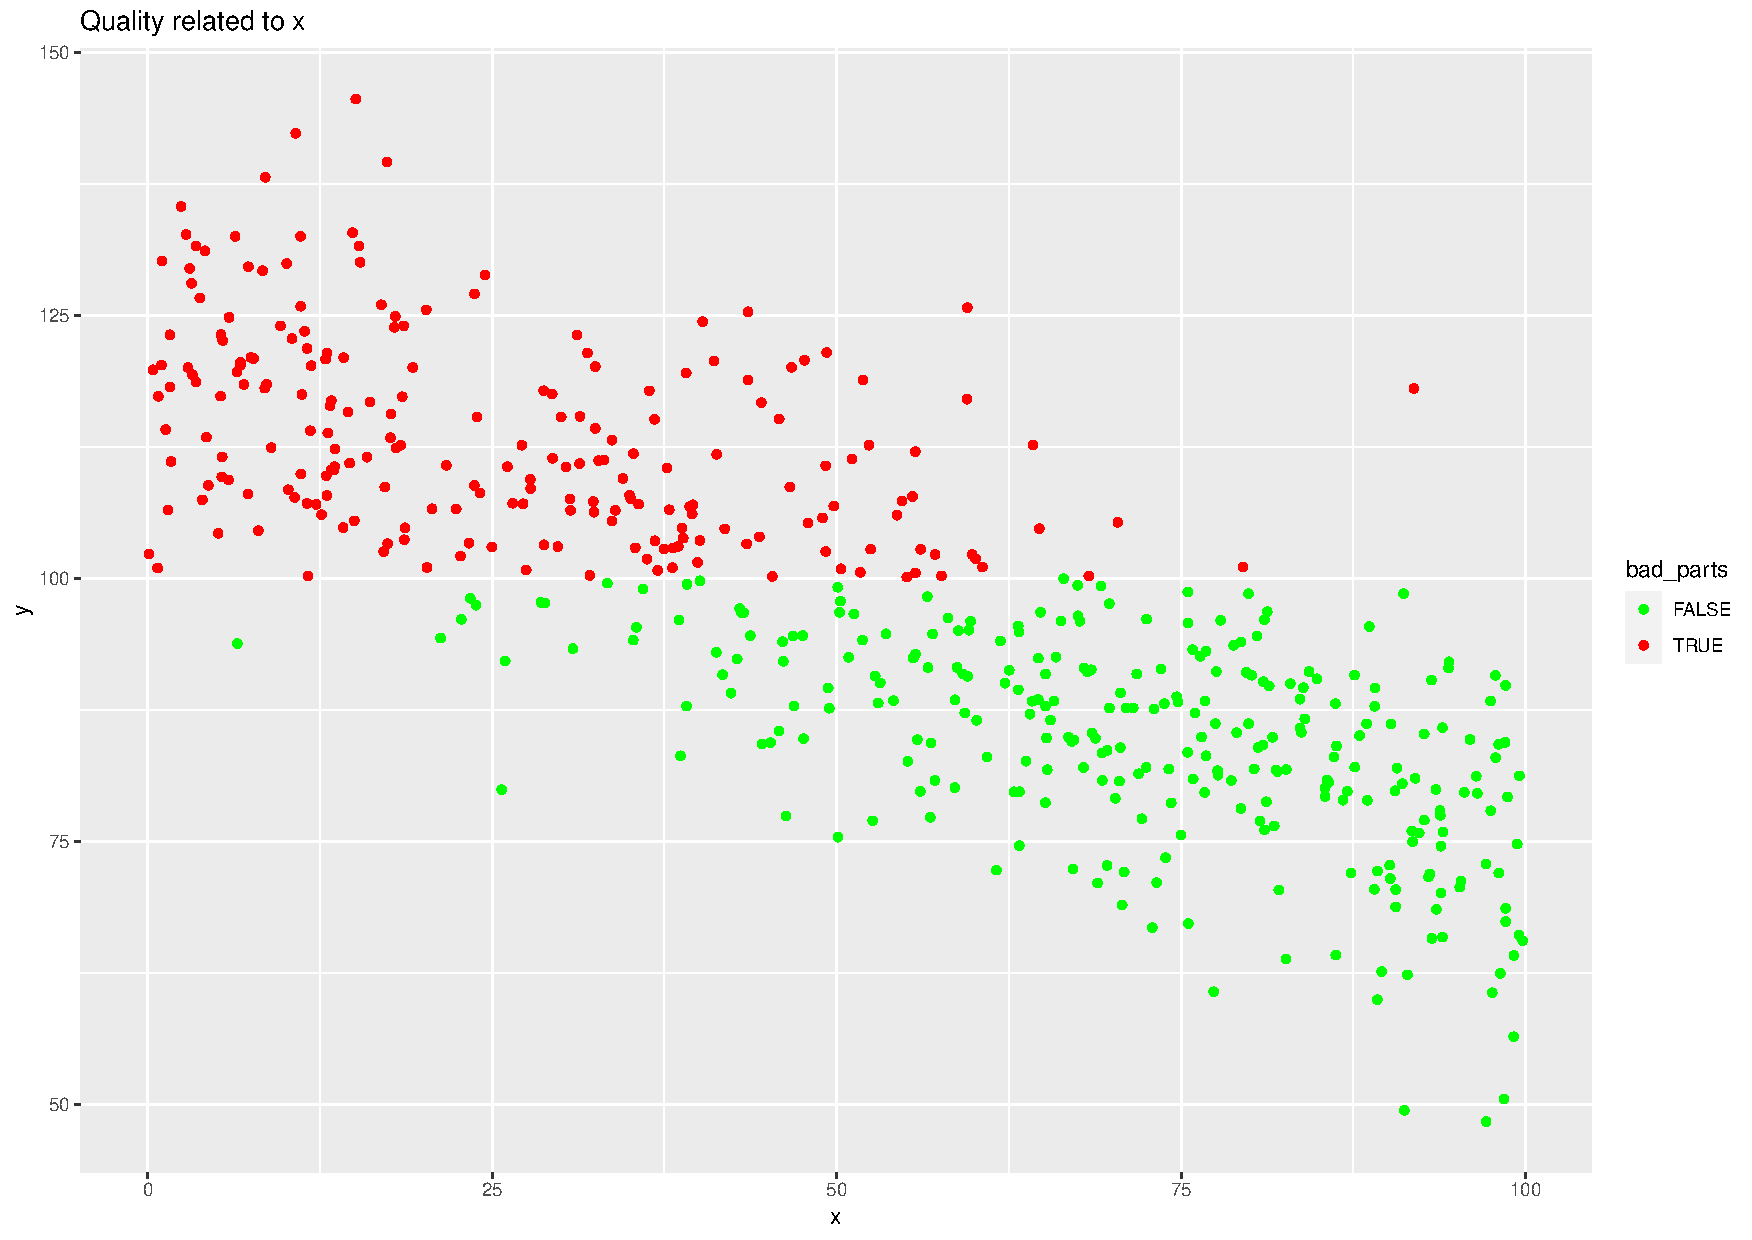
\includegraphics[width=0.95\textwidth]{bad-parts-r.pdf}
	\caption{Diagram of~the distribution of~parts with respect to~the parameter~\emph{x}.}
	\label{fig:bad-parts-r}
\end{figure}

The training sub-sample will~be used to~create a~logistic regression model based on~the values of~the attribute~\emph{x}, which allows you to~assign a~particular part to~quality or~defective. This model will~be used to~assign scores to~the observations in~the training sample. In~the future, these scores will~be used to~construct the ROC curve together with the true labels. Recall that the ROC curve is~plotted for observations with known values of~parameters \emph{x} and~\emph{y}. This ROC curve is~then applied to~the entire set of~objects for which x~values are known but y~values are unknown. The scores themselves as~well as~the~\emph{x} and \emph{y}~values are not displayed on~the graph and are only used for sorting labels. Two different classifiers sorting labels in~the same order will give identical ROC curves regardless of~the absolute values of~the scores. This can~be seen by~constructing an~ROC curve based on~"response" or~"link" predictions from a~logistic regression model. The "response" scores were mapped to~a~(0, 1) scale using a~\href{https://en.wikipedia.org/wiki/Sigmoid_function}{Sigmoid function}\cite{Wiki:sigmoid-function}, the "link" scores were left untransformed. In~this case, the points showing specific observations are ordered in~the same way. To test this hypothesis, we~use the code~\ref{lst:link-response-comparison}. As~you can see in~Figure~\ref{fig:link-response-comparison-r}, the order of~the dots is~the same for "link" and "response".
%
\begin{lstlisting}[float=htp, caption = Comparing "link" and "response" predictions, firstnumber=1, label= lst:link-response-comparison]
fit_glm <- glm(bad_parts ~ x, training_set, family=binomial(link="logit"))

glm_link_scores <- predict(fit_glm, test_set, type="link")

glm_response_scores <- predict(fit_glm, test_set, type="response")

score_data <- data.frame(link=glm_link_scores, 
response=glm_response_scores,
bad_parts=test_set$bad_parts,
stringsAsFactors=FALSE)

score_data %>% 
ggplot(aes(x=link, y=response, col=bad_parts)) + 
scale_color_manual(values=c("green", "red")) + 
geom_point() + 
geom_rug() + 
ggtitle("Both link and response scores put cases in the same order")

\end{lstlisting}
%
\begin{figure}[htp]
	\centering
	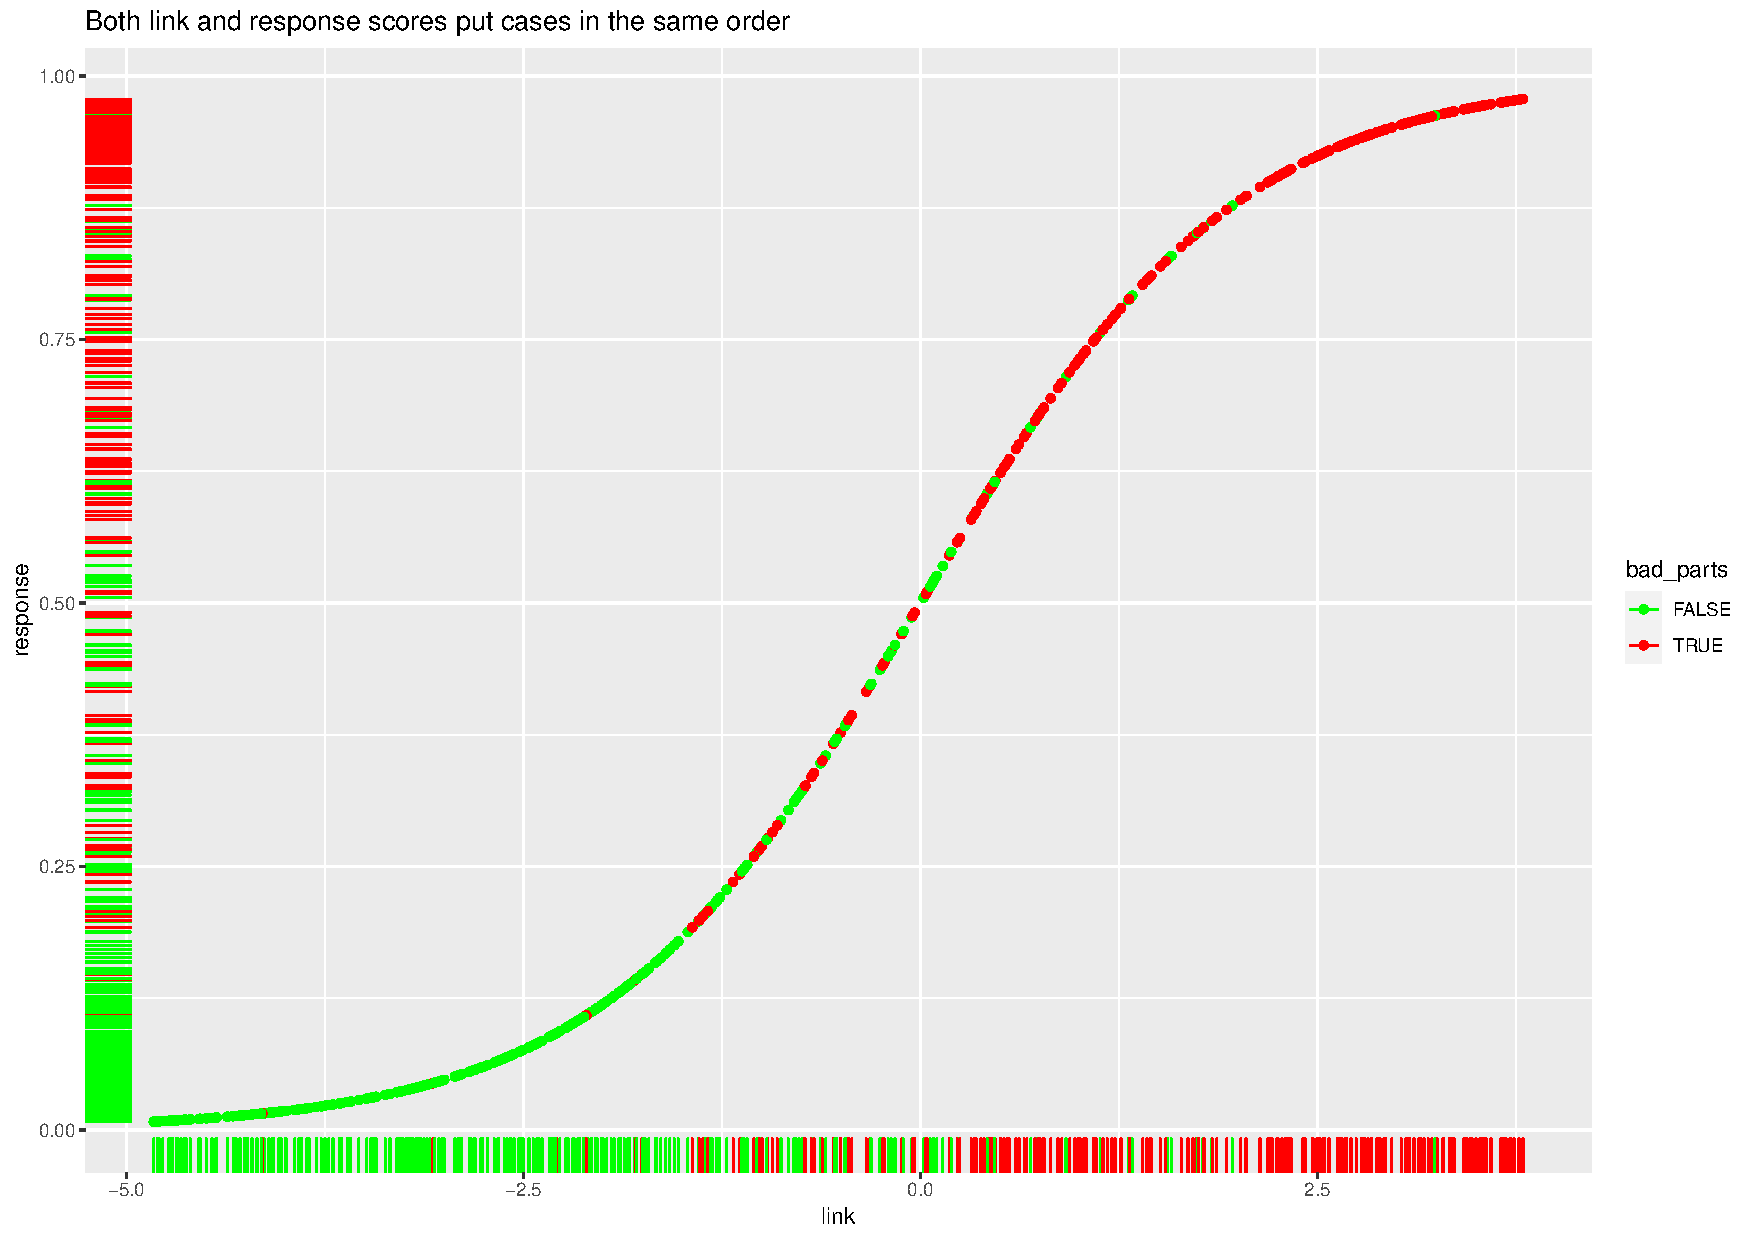
\includegraphics[width=0.95\textwidth]{link-response-comparison-r.pdf}
	\caption{Comparison of~the order of~points for "link" and "response".}
	\label{fig:link-response-comparison-r}
\end{figure}
%

Let's go directly to~the construction of~the ROC curve. We use both the ready function from the "pROC" package and the previously created \textbf{"appraiserRoc"} function (see script~\ref{lst:plot-ROC-1-r}). The result of~the first is~represented as~an~orange curve, the second as~circles of~red for defective parts and black for quality parts (see Diagram~\ref{fig:test-ROC-r}). It~is not difficult to~guess that the red dot corresponded to~the "North" command and the black dot to~the "East" command. Since the library function and the own function perform the same actions, the two curves are identical.

Note that the "Specificity" scale is~plotted on~the abscissa axis, not the FPR, so~the values on~the axis are inverted. Since, according to~Table~\ref{tab:ROC-rates-1}, $"Specificity = 1 - FPR"$ we can talk about the mutual unambiguity of~these indicators. Consequently, when plotting the ROC curve any of~them can~be used. This version of~the scale display was self-selected by~the \textbf{roc} function from the "pRoc" library. If~the user does not set his settings, the function chooses to~display the scale so~that the AUC value is~always greater than 0.5. This calculation is~based on~which group (quality parts, defective parts) has a~higher median score. Since the \textbf{appraiserRoc} function is~of~course not that smart, a~simple subtraction was performed during its use, making it~possible to~build a~joint diagram.

This approach has one limitation: based on~the prognostic nature of~the ordering of~outcomes, it~does not allow correct processing of~information if~the sequence consists of~identical estimates. "Turtle" assumes that the order of~the labels matters, but there is~no~meaningful order in~the situation of~the same scores. These areas should~be displayed with a~diagonal line, but not the traditional steps.
%
\begin{lstlisting}[float=htp, caption = Plotting the ROC curve using library and own functions, firstnumber=1, label= lst:plot-ROC-1-r]
# plot ROC
plot(roc(test_set$bad_parts, glm_response_scores, direction="<"),
col="orange", lwd=3, main="The turtle finds its way", xlim = c(1, 0))
glm_simple_roc <- appraiser_roc(test_set$bad_parts=="TRUE", glm_link_scores)
with(glm_simple_roc, points(1 - FPR, TPR, col=1 + labels))
\end{lstlisting}
%
\begin{figure}[htp]
	\centering
	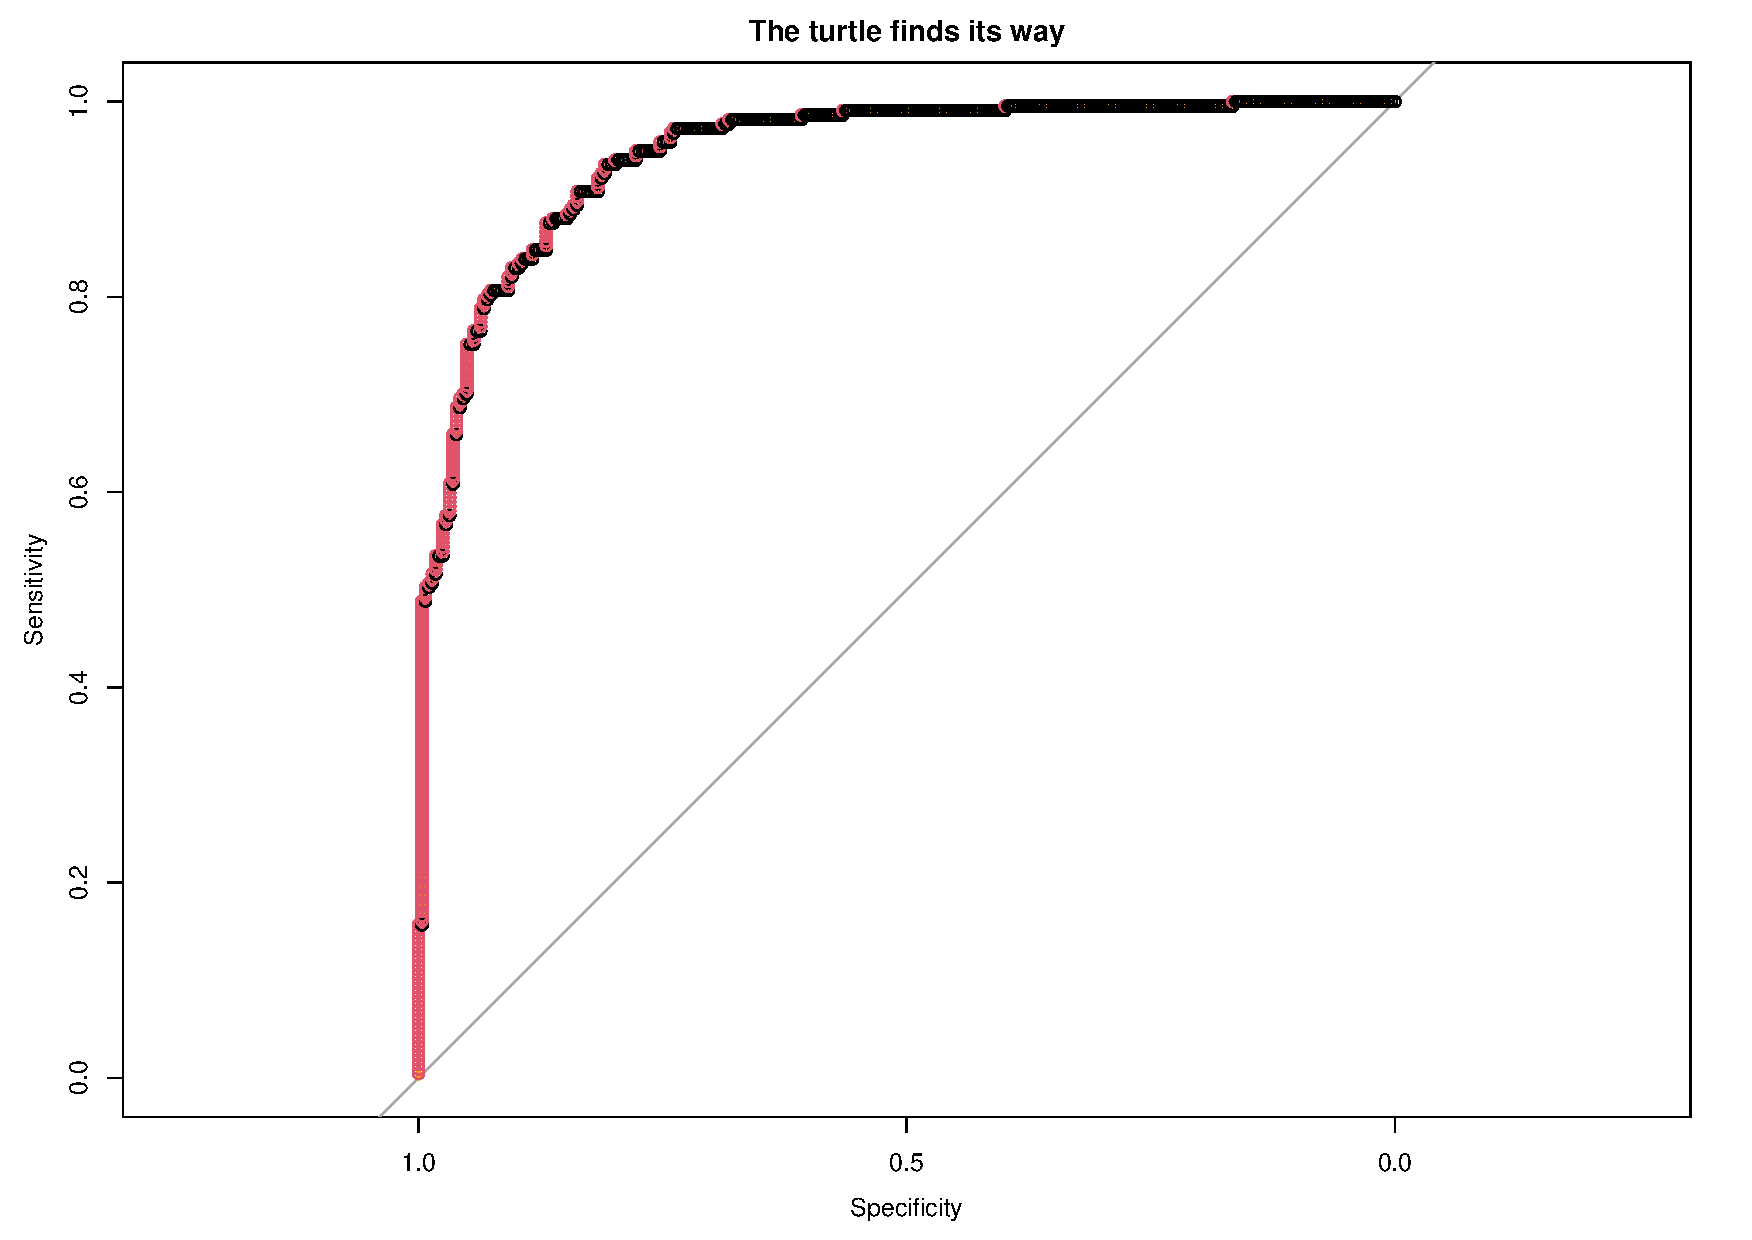
\includegraphics[width=0.95\textwidth]{test-ROC-r.pdf}
	\caption{Identical ROC curves plotted with library and own functions.}
	\label{fig:test-ROC-r}
\end{figure}
%

Consider an~example where a~diagonal is~the only adequate way to~plot a~ROC curve. To~do~this, create an~extremely unbalanced data set in~which only~1\,\% of~the observations are "positive". In~this case, the result of~the prediction will always be~negative. Since all scores will~be the same, there is~no~need for any ordering. The \textbf{roc} function from the "pRoc" package correctly recognizes such situations and draws a~diagonal line~(1,0; 0,1). In~doing so, the turtle assumes that the order of~scores has some significance, and moves between these points along a~random trajectory, alternating between "north" and "east" directions. The code calling the construction of~such a~ROC curve is~given in~script~\ref{lst:plot-ROC-rare-success-r}. In~Diagram~\ref{fig:ROC-rare-success-r}, the black diagonal line was plotted by~the library function, while the blue dashed line was plotted by~our own previously written \textbf{appraiserRoc} function.  As~you can see, the library function correctly determined the case of~identical estimates, while applying our own function resulted in~random turtle wanderings.
%
\begin{lstlisting}[float=htp, caption = Plotting the ROC curve in~case of~absence of~order of~scores, firstnumber=1, label= lst:plot-ROC-rare-success-r]
# plot ROC for 99% negative cases
N <- 2000
P <- 0.01
rare_success <- sample(c(TRUE, FALSE), N, replace=TRUE, prob=c(P, 1-P))
guess_not <- rep(0, N)
plot(roc(rare_success, guess_not), print.auc=TRUE)
appr_roc <- appraiserRoc(rare_success, guess_not)
with(appr_roc, lines(1 - FPR, TPR, col="blue", lty=2))
\end{lstlisting}
%
\begin{figure}[htp]
	\centering
	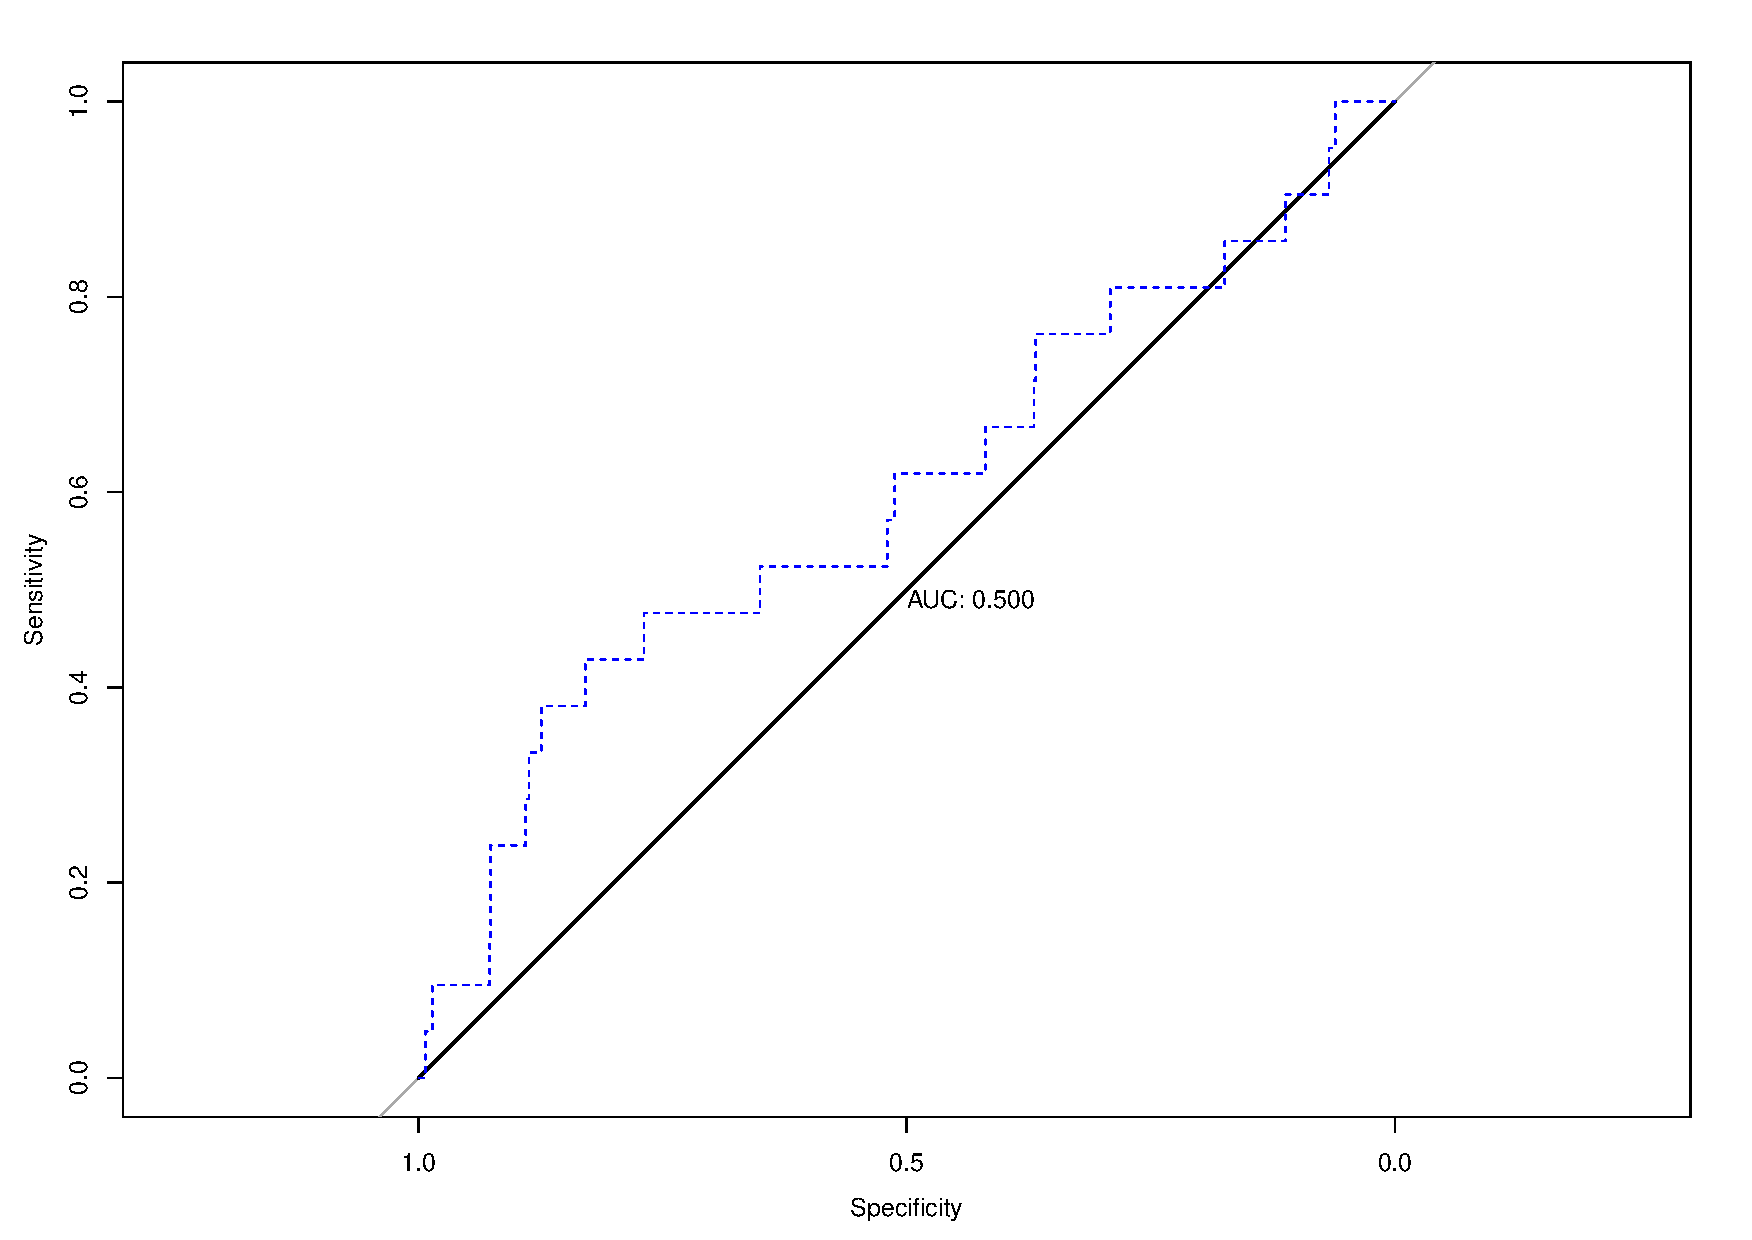
\includegraphics[width=0.95\textwidth]{ROC-rare-success-r.pdf}
	\caption{ROC curve arising when there is~no~value of~the order of~scores.}
	\label{fig:ROC-rare-success-r}
\end{figure}
%

The greater the value of~N, the closer to~the diagonal the turtle will wander. Greater unbalance requires more points in~order for the path to~run roughly close to~the diagonal. In~less extreme cases, the emergence of~diagonal sections is~possible, in~particular, in~the case of~rounding of~estimates, leading to~equality of~some of~them.

To further familiarize yourself with the topic of constructing ROC curves, we can recommend studying this \href{https://web.tresorit.com/l/APSpC#AfkTKO5_-ijMhPuXE-qEzg}{theoretical material}~\cite{ROC-analysis}, as~well as~practice on~the \href{https://kennis-research.shinyapps.io/ROC-Curves/}{online simulator}~\cite{ROC-curve-practice}.
%
\subsubsection{The concept of~AUC and its calculation}\label{calculate-AUC-theory}
The ROC curve is~a~popular means of~visualizing the trade-off between sensitivity and specificity of~a~binary classifier. Earlier in~\ref{plot-ROC-theory}, the issue of~constructing the ROC curve was considered in~terms of~the turtle steps, which takes a~vector with instructions as~steps "north", i.\,e., in~the positive direction on~the y-axis, and "east", i.\,e., in~the positive direction on~the x-axis. In~this case, the sequence of~scores, on~the basis of~which the vector of~bitwise instructions is~formed, is~ordered in~such a~way that the cases that are most likely to~be positive come first. In~doing so, the turtle assumes that all cases are positive. Next, for the training sample (in~which true values are known for certain), we~determine whether the case was true-~(TP) or~false-positive~(FP). The step size on~the y-axis is~inversely proportional to~the number of~positive observations, on~the x-axis to~the number of~negative observations. Thus, the curve path always ends at~(1,1). The result is~a~plot of~the frequency of~true positives (\textit{TPR} or~\textit{sensitivity}) against the frequency of~false positives (\textit{FPR} or~$1-specificity$), which is~actually the ROC curve. At~the same time, the graph itself does~not provide any quantitative estimates of~the quality of~the binary classifier.

Calculating the area under the ROC curve is~one way to~summarize the quantitative assessment of~classifier quality. This metric is~so~common that in~the context of~data analysis, the terms \emph{Area under the curve} or~\emph{AUC} refer specifically to~the area under the ROC curve, unless explicitly stated otherwise.

At~first glance, the simplest and most intuitive metric for classifier performance is~its accuracy. Unfortunately, in~some cases, such a~metric simply will not work. For example, in~the case of~a~disease that occurs in~one person per million, a~completely useless test that always shows a~negative result would~be 99.9999\% accurate. In~contrast to~the accuracy index, ROC curves are insensitive to~unbalanced classes. The aforementioned useless test will have an~$AUC=0.5$, which is~equivalent to~no~test at~all (see diagram~\ref{fig:ROC-rare-success-r}).

In~this subsubsection, we~will first consider the geometric approach to~the concept of~AUC and develop a~function that calculates its value. Next, we~turn to~another --- probabilistic --- interpretation of~the concept of~AUC.

\paragraph{Geometric approach to~the concept of~AUC}
First, let's create a~test dataset using the code shown in~\ref{lst:AUC-theory-create-dataset-r}.
%
\begin{lstlisting}[float=htp, caption = Create a~test data set, firstnumber=1, label= lst:AUC-theory-create-dataset-r]
# Geometric interpretation of AUC

# activate libraries
library(pROC)

# create dataset
category <- c(1, 1, 1, 1, 0, 1, 1, 0, 1, 0, 1, 0, 1, 0, 0, 1, 0, 0, 0, 0)
prediction <- rev(seq_along(category))
prediction[9:10] <- mean(prediction[9:10])
\end{lstlisting}
%
The \textbf{prediction} vector contains pseudo-estimates, which in~practice are assigned by~the classifier. In~this study problem, they are a~decreasing sequence, which generally corresponds to~the "category" labels. The scores for observations with ordinal numbers 9 and 10, one representing the positive case and the other the negative case, are replaced by~their mean values to~create a~ties effect.

To~construct the ROC curve, TPR and FPR must~be calculated. It~was shown in~\ref{plot-ROC-theory} how this can~be done semi-automatically by~calculating cumulative sums for positive and negative labels. This section will use the library "pRoc", which performs all calculations automatically at~a~low level. Let's calculate the TPR, FPR, and AUC values with the code~\ref{lst:AUC-as-geom-calculate-AUC-r}. A~dataframe will also~be created, containing the data for each observation, and shown in~Table~\ref{tab:roc_df-r}. The \textbf{roc} function can return the values of~many indicators, but at~this point we only need TPR and FPR. Recall that TPR means sensitivity and FPR is~equivalent to~the expression $1 - specificity$. By~default, the \textbf{roc} function returns values in~ascending order. As~a~consequence, they have been inverted so~that the starting point has coordinates~(0,0). The AUC value returned by~the function was~0.825. In~the following, we will compare it with the one that will~be obtained in the course of~its independent semi-automatic calculation.
%
\begin{lstlisting}[float=htp, caption = Calculation of~the AUC using the pRoc library, firstnumber=1, label= lst:AUC-as-geom-calculate-AUC-r]
# create ROC object&dataframe and calculate AUC
roc_obj <- roc(category, prediction)
auc(roc_obj)
roc_df <- data.frame(
TPR=rev(roc_obj$sensitivities), 
FPR=rev(1 - roc_obj$specificities), 
labels=roc_obj$response, 
scores=roc_obj$predictor)
\end{lstlisting}
%
\begin{table}[htp]
	\caption{TPR, FPR, labels, scores for the training dataset.}\label{tab:roc_df-r}
	\centering
	\begin{tabular}{lllll}
		\hline
		& TPR & FPR & labels & scores \\ 
		\hline
		1 & 0.00 & 0.00 & 1.00 & 20.00 \\ 
		2 & 0.10 & 0.00 & 1.00 & 19.00 \\ 
		3 & 0.20 & 0.00 & 1.00 & 18.00 \\ 
		4 & 0.30 & 0.00 & 1.00 & 17.00 \\ 
		5 & 0.40 & 0.00 & 0.00 & 16.00 \\ 
		6 & 0.40 & 0.10 & 1.00 & 15.00 \\ 
		7 & 0.50 & 0.10 & 1.00 & 14.00 \\ 
		8 & 0.60 & 0.10 & 0.00 & 13.00 \\ 
		9 & 0.60 & 0.20 & 1.00 & 11.50 \\ 
		10 & 0.70 & 0.30 & 0.00 & 11.50 \\ 
		11 & 0.80 & 0.30 & 1.00 & 10.00 \\ 
		12 & 0.80 & 0.40 & 0.00 & 9.00 \\ 
		13 & 0.90 & 0.40 & 1.00 & 8.00 \\ 
		14 & 0.90 & 0.50 & 0.00 & 7.00 \\ 
		15 & 0.90 & 0.60 & 0.00 & 6.00 \\ 
		16 & 1.00 & 0.60 & 1.00 & 5.00 \\ 
		17 & 1.00 & 0.70 & 0.00 & 4.00 \\ 
		18 & 1.00 & 0.80 & 0.00 & 3.00 \\ 
		19 & 1.00 & 0.90 & 0.00 & 2.00 \\ 
		20 & 1.00 & 1.00 & 0.00 & 1.00 \\ 
		\hline
	\end{tabular}
\end{table}
%
\subparagraph{Plotting the graph}
If~the ROC curve were a~perfect step function, the area under it could~be found by adding a~set of~vertical bars equal to~the spaces between the points on~the abscissa axis (FPR) and to~the height of~the step on~the ordinate axis (TPR). Real ROC curves may include sections corresponding to~repeated values. In~this case, there are segments other than steps. Such repeats require proper consideration. In~Figure~\ref{fig:ROC-bars-R}, the area of~ordinary steps is~shown in~green, the cases of~repeats~(ties) are indicated by~blue rectangles divided in~half by~sloping ROC curve segments. Thus, half of~the area of~these steps is~included in~the total area under the curve.
%
\begin{figure}[htp]
	\centering
	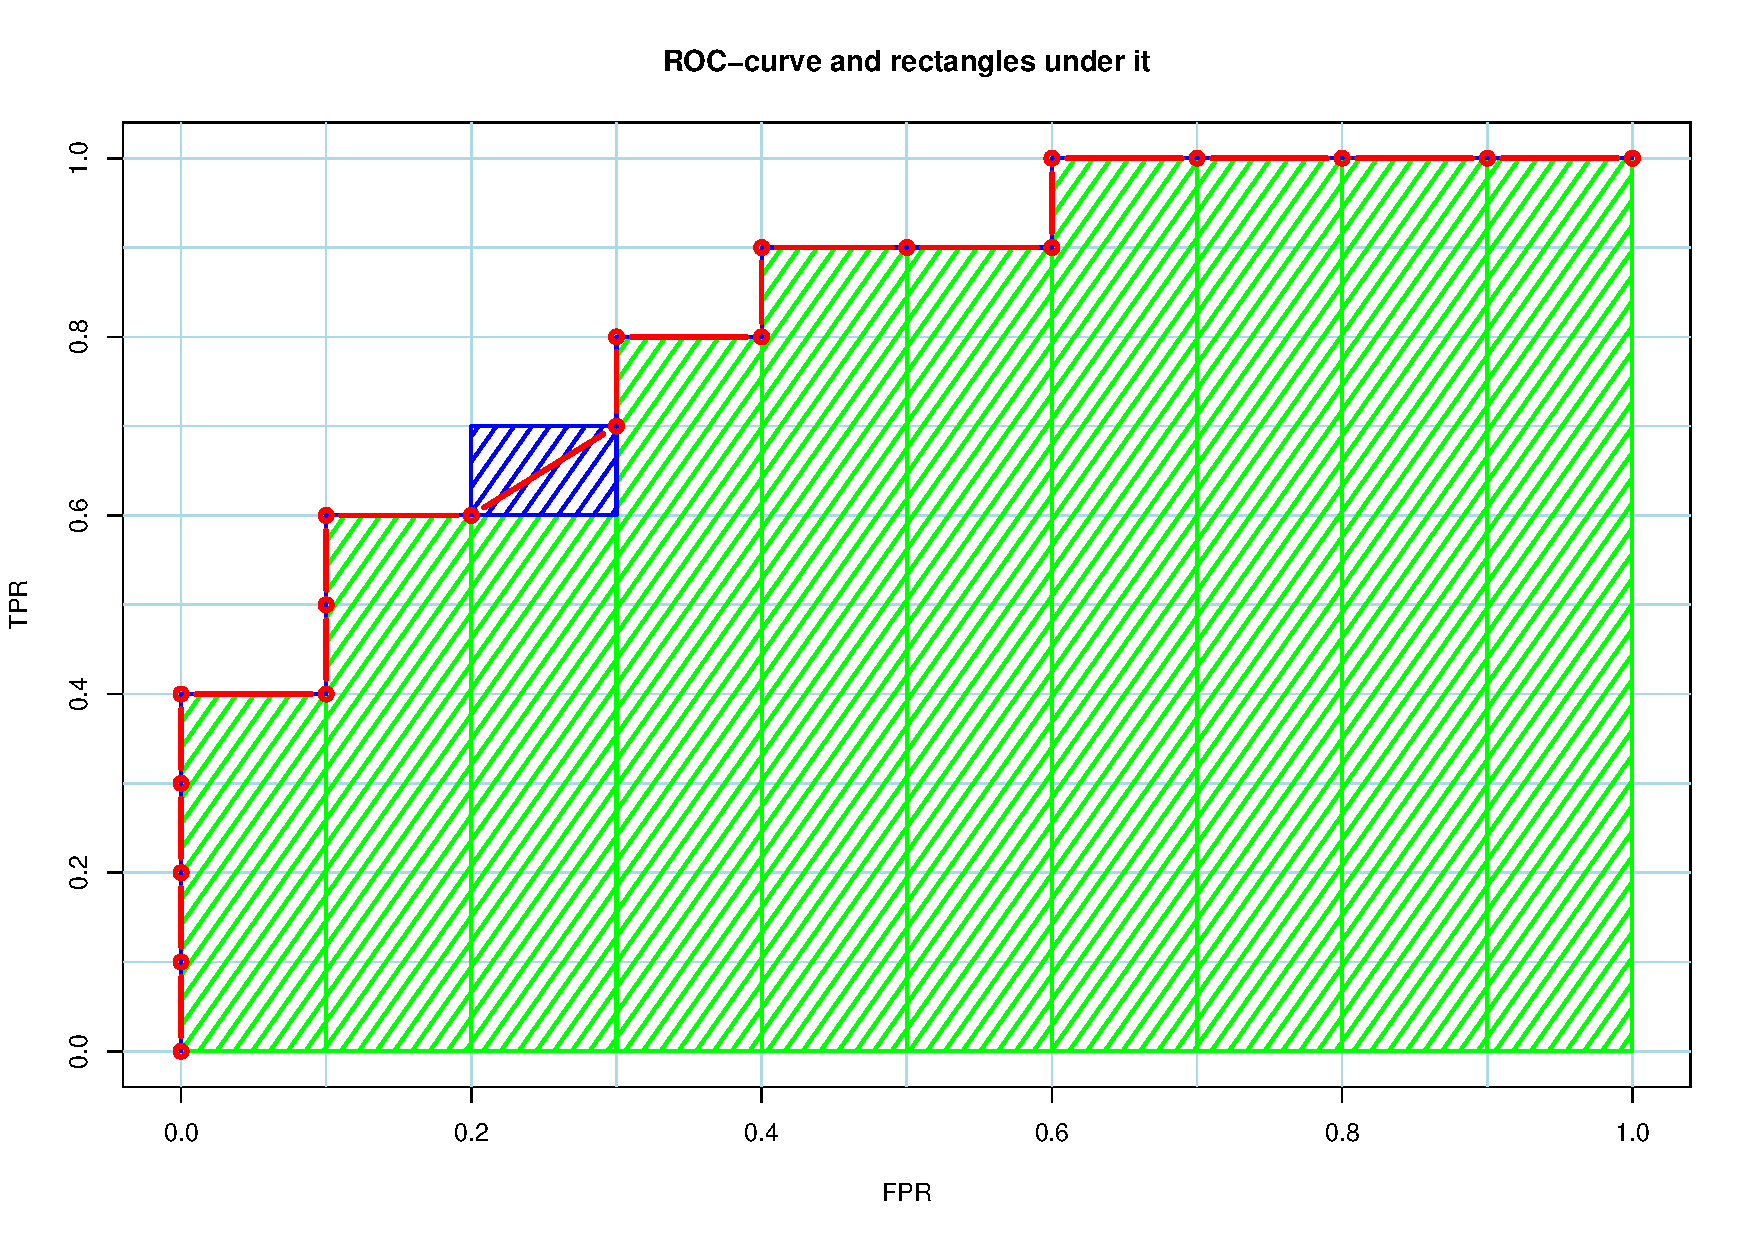
\includegraphics[width=0.95\textwidth]{ROC-bars-R.pdf}
	\caption{ROC curve and the area under it, taking into account the presence of~ties.}
	\label{fig:ROC-bars-R}
\end{figure}

The following steps were taken to~plot diagram~\ref{fig:ROC-bars-R}.
\begin{enumerate}
	\item Define a~\textbf{rectangle} function that takes as~arguments:
	\begin{itemize}
		\item the initial \emph{x} and~\emph{y} coordinates;
		\item width and height of~step;
		\item angle of~rotation after each step;
		\item hatching density.
	\end{itemize}
	The algorithm in~script~\ref{lst:create-rectangle-function-r} builds the rectangle as~follows:
	\begin{itemize}
		\item the function accepts the initial \emph{x} and~\emph{y} coordinates from the appraiser.
		\item then it gets the value of~the step length "to the east" (to~the right on the x-axis), calculates the new value of~the x-coordinate, keeping the value of~the y-coordinate.
		\item after performing the step is~a~turn of~45\textdegree counterclockwise.
		\item then it~gets the value of~the step length "to the North" (up~on~the y-axis), calculates a~new value of~the y-coordinate, keeping the value of~the x-coordinate.
		\item this~is followed by~a~new turn to~the left by~45\textdegree and new steps in~opposite directions.
		\item thus, performing one step each to~the “east”, “north”, “west” and “south”, as~well as~three turns of~45\textdegree counterclockwise function returns to~the starting point, completing the construction of~the rectangle.
	\end{itemize}
	\item To~calculate the step length "to~the East" and "to~the West" it~is necessary to~calculate the difference between neighboring values of~FPR, "to~the North" and "to~the South" between neighboring values of~TPR. To~do~this, we add the two columns \emph{dFPR} and \emph{dTPR}, respectively, using the code shown in~\ref{lst:add-dFPR&dTPR-columns-r}. Since the number of~pairs for which the difference is~calculated is~less than the number of~observations by~one, zero should~be added at~the end (since the dataframe data are sorted in~descending order).
	\item Next, the coordinate grid is~laid out from zero to~one on~each axis using the code~\ref{lst:plot-empty-graph-from-0-to-1-r}.
	\item For the case of~repeating values~(ties), there is~a~special kind of~step "to~the North-East" in~the form of~a~diagonal line.
	\item The final step is~to~build the ROC curve itself and the rectangles that form the area under~it, according to~script~~\ref{lst:plot-ROC-curve-and-rectangles-under-it-r}. The \textbf{mapply} function allows you to~apply the \textbf{rectangle} function sequentially to~each row of~the data frame.
\end{enumerate}
%
\begin{lstlisting}[float=htp, caption = Create the \textbf{rectangle} function, firstnumber=1, label= lst:create-rectangle-function-r]
# create function for plotting rectangles
rectangle <- function(x, y, width, height, density=12, angle=45, ...) 
polygon(c(x,x+width,x+width,x), c(y,y,y+height,y+height), 
density=density, angle=angle, ...)
\end{lstlisting}
%
\begin{lstlisting}[float=htp, caption = Adding \textit{dFPR} and \textit{dTPR} columns, firstnumber=1, label= lst:add-dFPR&dTPR-columns-r]
# add dFPR and dTPR columns
roc_df <- transform(roc_df, 
dFPR = c(diff(FPR), 0),
dTPR = c(diff(TPR), 0))
\end{lstlisting}
%
\begin{lstlisting}[float=htp, caption = Drawing an~empty graph and marking axes from~0 to~1, firstnumber=1, label= lst:plot-empty-graph-from-0-to-1-r]
# plot empty graph from 0 to 1 for each axis
plot(0:10/10, 0:10/10, type='n', xlab="FPR", ylab="TPR",
main = 'ROC-curve and rectangles under it')
abline(h=0:10/10, col="lightblue")
abline(v=0:10/10, col="lightblue")
\end{lstlisting}
%
\begin{lstlisting}[float=htp, caption = Construction of~ROC curve and rectangles under~it, firstnumber=1, label= lst:plot-ROC-curve-and-rectangles-under-it-r]
# plot ROC-curve and rectangles under it
with(roc_df, {
mapply(rectangle, x=FPR, y=0,   
width=dFPR, height=TPR, col="green", lwd=2)
mapply(rectangle, x=FPR, y=TPR, 
width=dFPR, height=dTPR, col="blue", lwd=2)
lines(FPR, TPR, type='b', lwd=3, col="red")
})
\end{lstlisting}

\subparagraph{The summation of~areas by~means of~an~own function}
The area under the curve~(AUC) (highlighted in~red) is~the sum of~the areas of~all the green rectangles and half the area of~the blue one. To~calculate the area of~each rectangle it~is not necessary to~know the absolute coordinates of~its vertices, its width and height are enough. Since one of~the sides of~each rectangle lies on~the x-axis, the height of~any of~them is~determined by~the value of~TPR, the width by~dFPR. Then the total area of~all green rectangles is~equal to~the \href{https://en.wikipedia.org/wiki/Dot_product}{dot~(scalar) product}~\cite{Wiki:dot-product} of~TPR and dFPR. This vector approach calculates the area for each data point, even if~its width or~height is~zero. However, in~this case their further inclusion in~the calculation is of no~importance. The area of~the blue rectangles (if~any) is~determined by~the values of~dFPR and dTPR and also represents their scalar product as~vectors. For areas of~the graph containing northward or~eastward steps, one of~these values (dTPR, dFPR) will~be zero. As~a~consequence, blue rectangles are possible only if~TPR and FPR are changed simultaneously. In~this case, only half of~such rectangle is~under the curve.

Recall that the previously calculated AUC was~0.825. Now let's calculate it in~semi-automatic mode according to~the algorithm described in the previous paragraph. To~do this, first create the function \textbf{appraiser\_auc}, and then apply it to~the test data (see script~\ref{lst:create&apply-appraiser-auc-function-r}). The returned value will~be~0.825, which indicates that the logic and algorithm are correct.
%
\begin{lstlisting}[float=htp, caption = Creating a function to calculate AUC in semi-automatic mode and applying it to test data, firstnumber=1, label= lst:create&apply-appraiser-auc-function-r]
# create function for AUC calculation
appraiser_auc <- function(TPR, FPR){
# inputs already sorted, best scores first 
dFPR <- c(diff(FPR), 0)
dTPR <- c(diff(TPR), 0)
sum(TPR * dFPR) + sum(dTPR * dFPR)/2
}

# apply function to data
with(roc_df, appraiser_auc(TPR, FPR))
\end{lstlisting}

\paragraph{The rank comparison approach}
It~is also possible to~use a~fundamentally different approach to~calculate the AUC. To~implement~it, it~is necessary to~create a~matrix containing all possible combinations of~positive and negative cases. Each row represents a~positive case. They are ordered so that the top row contains the case with the lowest score, and the bottom row contains the case with the highest score. Similarly, the columns contain the negative cases, sorted so that the left column contains the highest scores. Then each cell represents a~comparison of~a~particular positive case with a~particular negative case. If~the score or rank of~a~positive case is higher than that of~a~negative case, that cell takes TRUE. In the case of a~good enough classifier, most positive cases will have higher scores (ranks) than negative cases. All exceptions will~be concentrated in the upper left corner, where positive cases with low scores and negative cases with high scores are located. The~\ref{lst:rank_comparison_auc-r} script contains code to~implement this algorithm and its visualization, shown in~Figure~\ref{fig:rank-comparison-matrix-vizualization-r}.
%
\begin{lstlisting}[float=htp, caption = Create the function to~build a~comparison matrix and apply it to~the test data, firstnumber=1, label= lst:rank_comparison_auc-r]
# create  function for rank comparison
rank_comparison_auc <- function(labels, scores, plot_image=TRUE, ...){
score_order <- order(scores, decreasing=TRUE)
labels <- as.logical(labels[score_order])
scores <- scores[score_order]
pos_scores <- scores[labels]
neg_scores <- scores[!labels]
n_pos <- sum(labels)
n_neg <- sum(!labels)
M <- outer(sum(labels):1, 1:sum(!labels), 
function(i, j) (1 + sign(pos_scores[i] - neg_scores[j]))/2)

AUC <- mean (M)
if (plot_image){
image(t(M[nrow(M):1,]), ...)
library(pROC)
with( roc(labels, scores),
lines((1 + 1/n_neg)*((1 - specificities) - 0.5/n_neg), 
(1 + 1/n_pos)*sensitivities - 0.5/n_pos, 
col="blue", lwd=2, type='b'))
text(0.5, 0.5, sprintf("AUC = %0.4f", AUC))
}

return(AUC)
}

# apply function to data
rank_comparison_auc(labels=as.logical(category), scores=prediction)
\end{lstlisting}
%
\begin{figure}[htp]
	\centering
	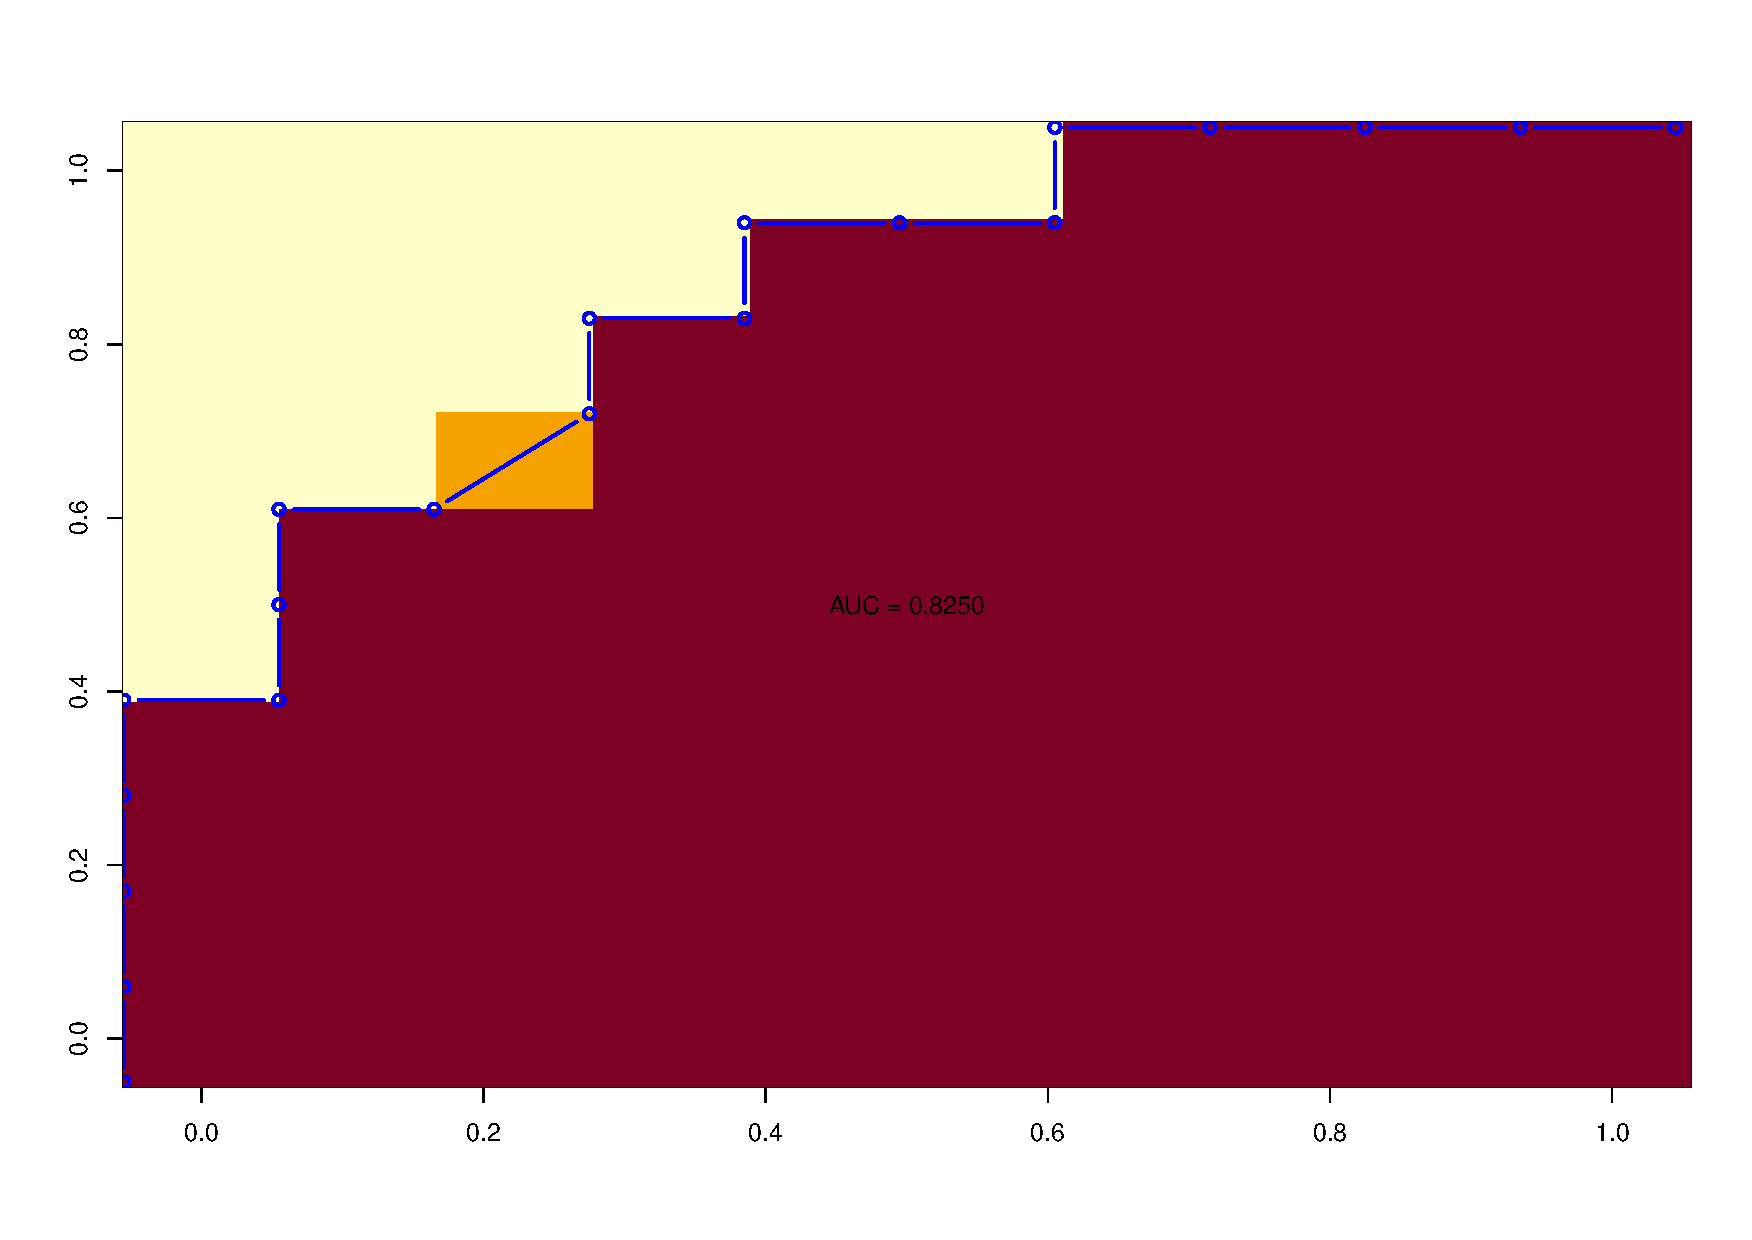
\includegraphics[width=0.95\textwidth]{rank-comparison-matrix-vizualization-r.pdf}
	\caption{Visualization of~the matrix of~comparisons of~scores (ranks).}
	\label{fig:rank-comparison-matrix-vizualization-r}
\end{figure}
%

The plotting of~the ROC curve in~this case is~done almost in the usual way. The only difference is that it~is slightly shifted and stretched to~make the coordinates coincide with the corners of~the matrix cells. This way of~constructing the ROC curve makes the following fact obvious: the ROC curve represents the boundary of the area where positive cases have higher scores (ranks) than negative cases. Thus, the AUC can~be calculated by replacing the values in the matrix so that
\begin{itemize}
	\item cells in which the scores (ranks) of positive cases exceed the scores (ranks) of negative cases take the value~1;
	\item cells in which the scores (ranks) are equal take the value~0.5;
	\item cells in which the scores (ranks) of negative cases exceed the scores (ranks) of positive cases take the value~0.
\end{itemize}
Since applying the \textbf{sign} function results in one of three possible values: -1, 0, 1, we use the following trick to place the values in the desired range: we add one to them and divide by two. The final calculation of the AUC is done by calculating the mean value.

\paragraph{Probabilistic approach to calculating AUC}
The probabilistic interpretation is that if you randomly choose a~positive case and a~negative case, the probability that the score (rank) value of the positive case will~be greater than that of the negative case is determined by AUC and equal to it. This follows, in particular, from Diagram~\ref{fig:rank-comparison-matrix-vizualization-r}, in which the total area of the graph is normalized to one. The total area of the graph is normalized to one, the cells of the matrix contain information about all possible combinations of positive and negative cases. The area under the curve consists of cells in which the scores (ranks) of positive cases exceed those of negative cases. To approximate the AUC in the probabilistic approach, let's create and apply a~function according to the script~\ref{lst:create&apply-auc-as-probability-r}. The returned AUC value was 0.8248116, which approximately corresponds to its exact value calculated earlier.
%
\begin{lstlisting}[float=htp, caption = Creating and applying a~function to calculate AUC as a~probability, firstnumber=1, label= lst:create&apply-auc-as-probability-r]
# create function for calculation AUC as probability
auc_probability <- function(labels, scores, N=1e7){
pos <- sample(scores[labels], N, replace=TRUE)
neg <- sample(scores[!labels], N, replace=TRUE)
# sum( (1 + sign(pos - neg))/2)/N # does the same thing
(sum(pos > neg) + sum(pos == neg)/2) / N # give partial credit for ties
}

# apply function to data
auc_probability(as.logical(category), prediction)
\end{lstlisting}
%

\subsubsection{Calculation of AUC for large data sets}
In the previous sections, we worked with a~very small dataset that allowed us to almost manually go through the data. In this subsubsection, we will work with a~previously created dataset containing information about quality and defective parts that require different valuation methods. Recall that in this dataset, the score vector is contained in the \textit{glm\_responce\_scores} variable, and the label vector is contained in the \textit{bad\_parts} variable.

The previously created dataset does not contain repeating values. Therefore, the tie effect will~be added artificially to explore the issue more deeply. For this purpose, rounding of scores was performed. Then we plot the ROC curve for the original data and then for the rounded data. The code to perform the above actions is given in script~\ref{lst:bad-parts-ROC-oroginal&rounded-r}. To create a~tie effect, a~new vector of scores was created, containing their values rounded to one decimal place. The result of plotting the two ROC curves is shown in Diagram~\ref{fig:bad-parts-ROC-original&rounded-r}. The black line corresponds to the ROC curve plotted from the original data. These data contain unique scores for each observation. The red line corresponds to the ROC curve plotted with rounded scores. As an input vector we used the data of variable 5, taking a value from 0 to 1. Consequently, scores rounded to one decimal place have only eleven possible values from~0.0 to~1.0. The AUC value for both cases is plotted directly on the chart. As can~be seen, the values are approximately equal due to a~sufficiently large number of observations.
%
\begin{lstlisting}[float=htp, caption = Plotting the ROC curve on the original (black line) and rounded (red line) defective parts data, firstnumber=1, label= lst:bad-parts-ROC-oroginal&rounded-r]
# create function for calculation AUC as probability
auc_probability <- function(labels, scores, N=1e7){
pos <- sample(scores[labels], N, replace=TRUE)
neg <- sample(scores[!labels], N, replace=TRUE)

# sum( (1 + sign(pos - neg))/2)/N # does the same thing
(sum(pos > neg) + sum(pos == neg)/2) / N # give partial credit for ties
}

# apply function to data
auc_probability(as.logical(category), prediction)
\end{lstlisting}
%
\begin{figure}[htp]
	\centering
	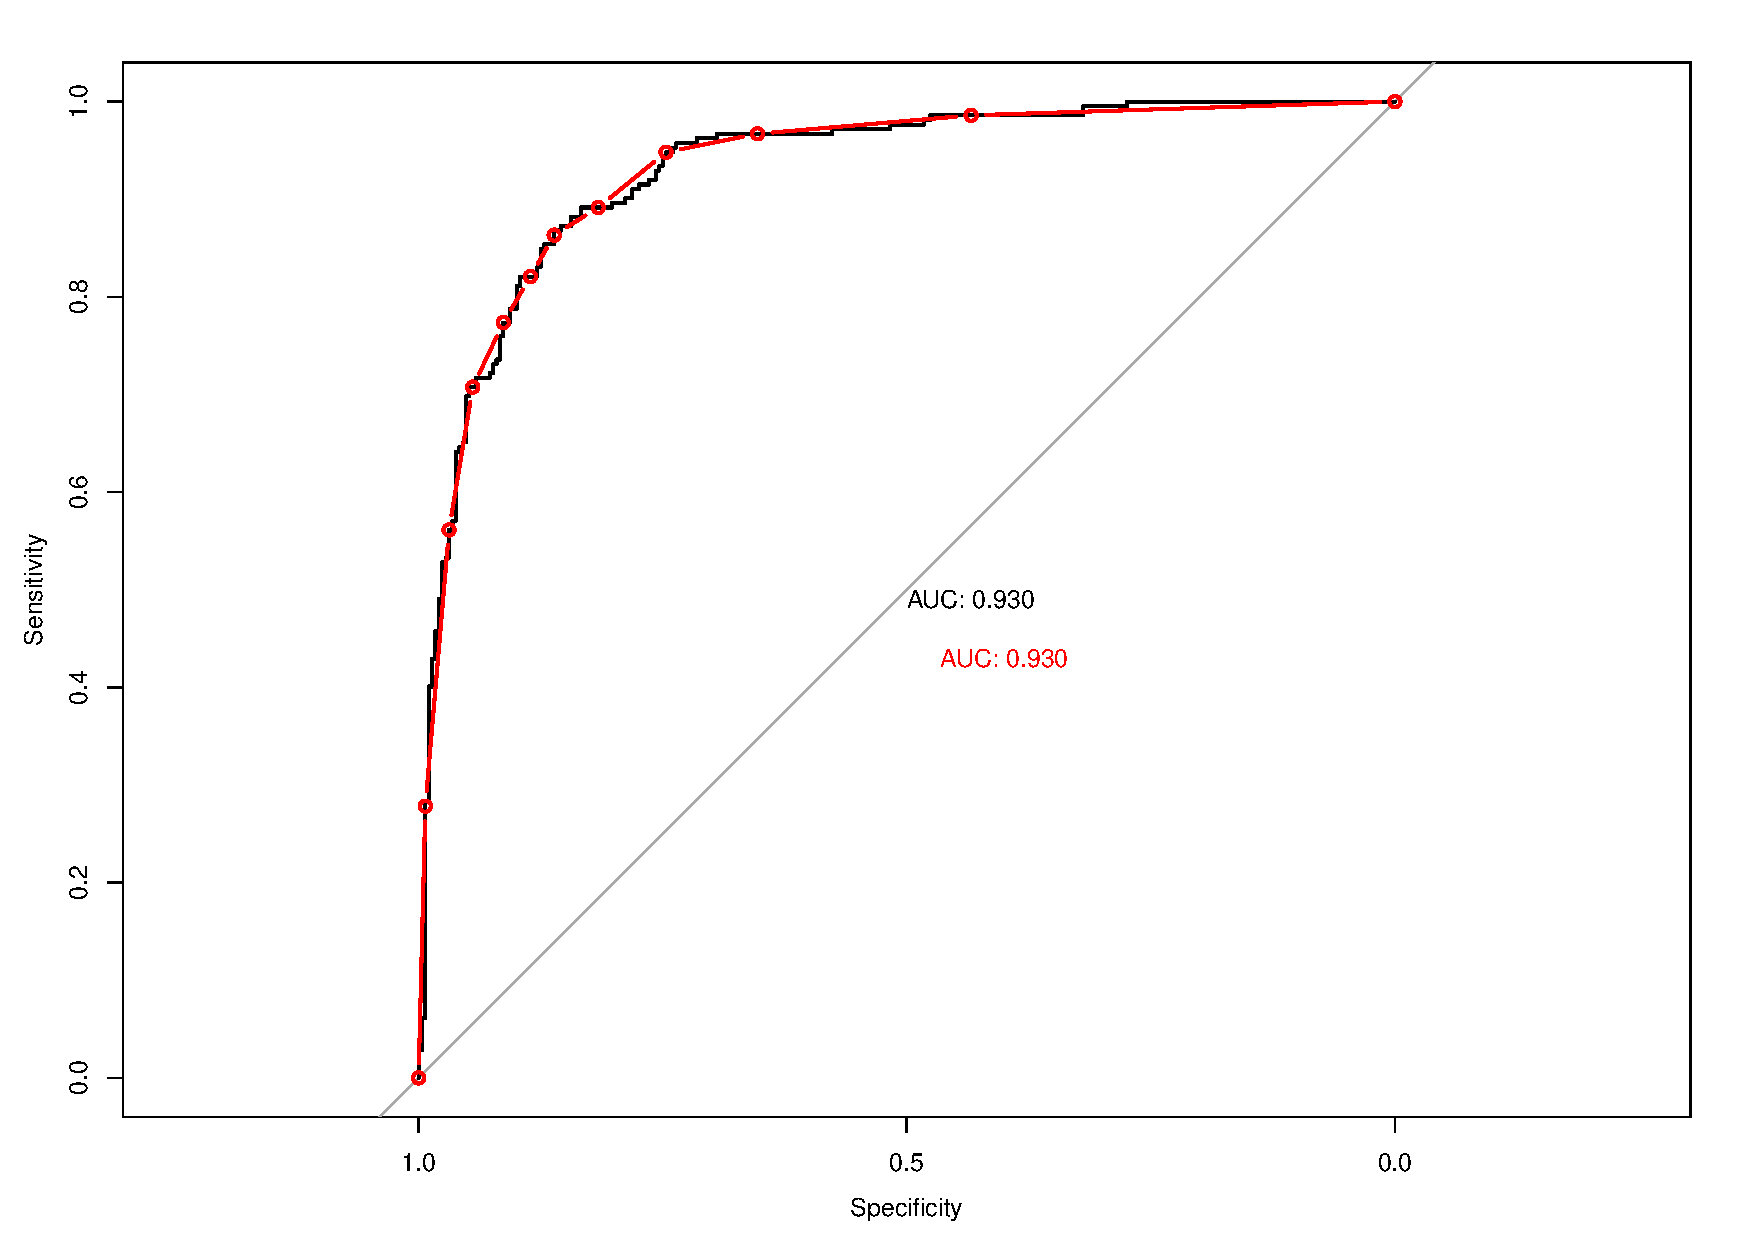
\includegraphics[width=0.95\textwidth]{bad-parts-AUC-ties.pdf}
	\caption{ROC curve for original (black line) and rounded (red line) data about defective parts.}
	\label{fig:bad-parts-ROC-original&rounded-r}
\end{figure}
%

Next, let's try to apply the standard, as well as three of our own functions to calculate the AUC. Next, we construct two ROC curves based on the rank comparison matrices for the original and rounded scores. The code for applying the four functions to calculate AUC, as well as constructing ROC curves based on comparison matrices, is given in script~\ref{lst:bad-parts-aplly-four-functions-r}.
%
\begin{lstlisting}[float=htp, caption = Using four functions to calculate AUC and plot ROC curves based on comparison matrices for original and rounded scores, firstnumber=1, label= lst:bad-parts-aplly-four-functions-r]
# apply all functions to data
results <- data.frame(
`Full Resolution` = c(
auc = as.numeric(auc(roc_full_resolution)),
appraiser_auc = appraiser_auc(rev(roc_full_resolution$sensitivities),
rev(1 - roc_full_resolution$specificities)),
rank_comparison_auc = rank_comparison_auc(test_set$bad_parts,
glm_response_scores, 
main="Full-resolution scores (no ties)"),
auc_probability = auc_probability(as.logical(test_set$bad_parts),
glm_response_scores)
),
`Rounded Scores` = c( 
auc = as.numeric(auc(roc_rounded)),
appraiser_auc = appraiser_auc(rev(roc_rounded$sensitivities),
rev(1 - roc_rounded$specificities)),
rank_comparison_auc = rank_comparison_auc(test_set$bad_parts, rounded_scores,
main="Rounded scores (ties in all segments)"),
auc_probability = auc_probability(as.logical(test_set$bad_parts),
rounded_scores)
)
)
\end{lstlisting}
%
\begin{figure}[htp]
	\centering
	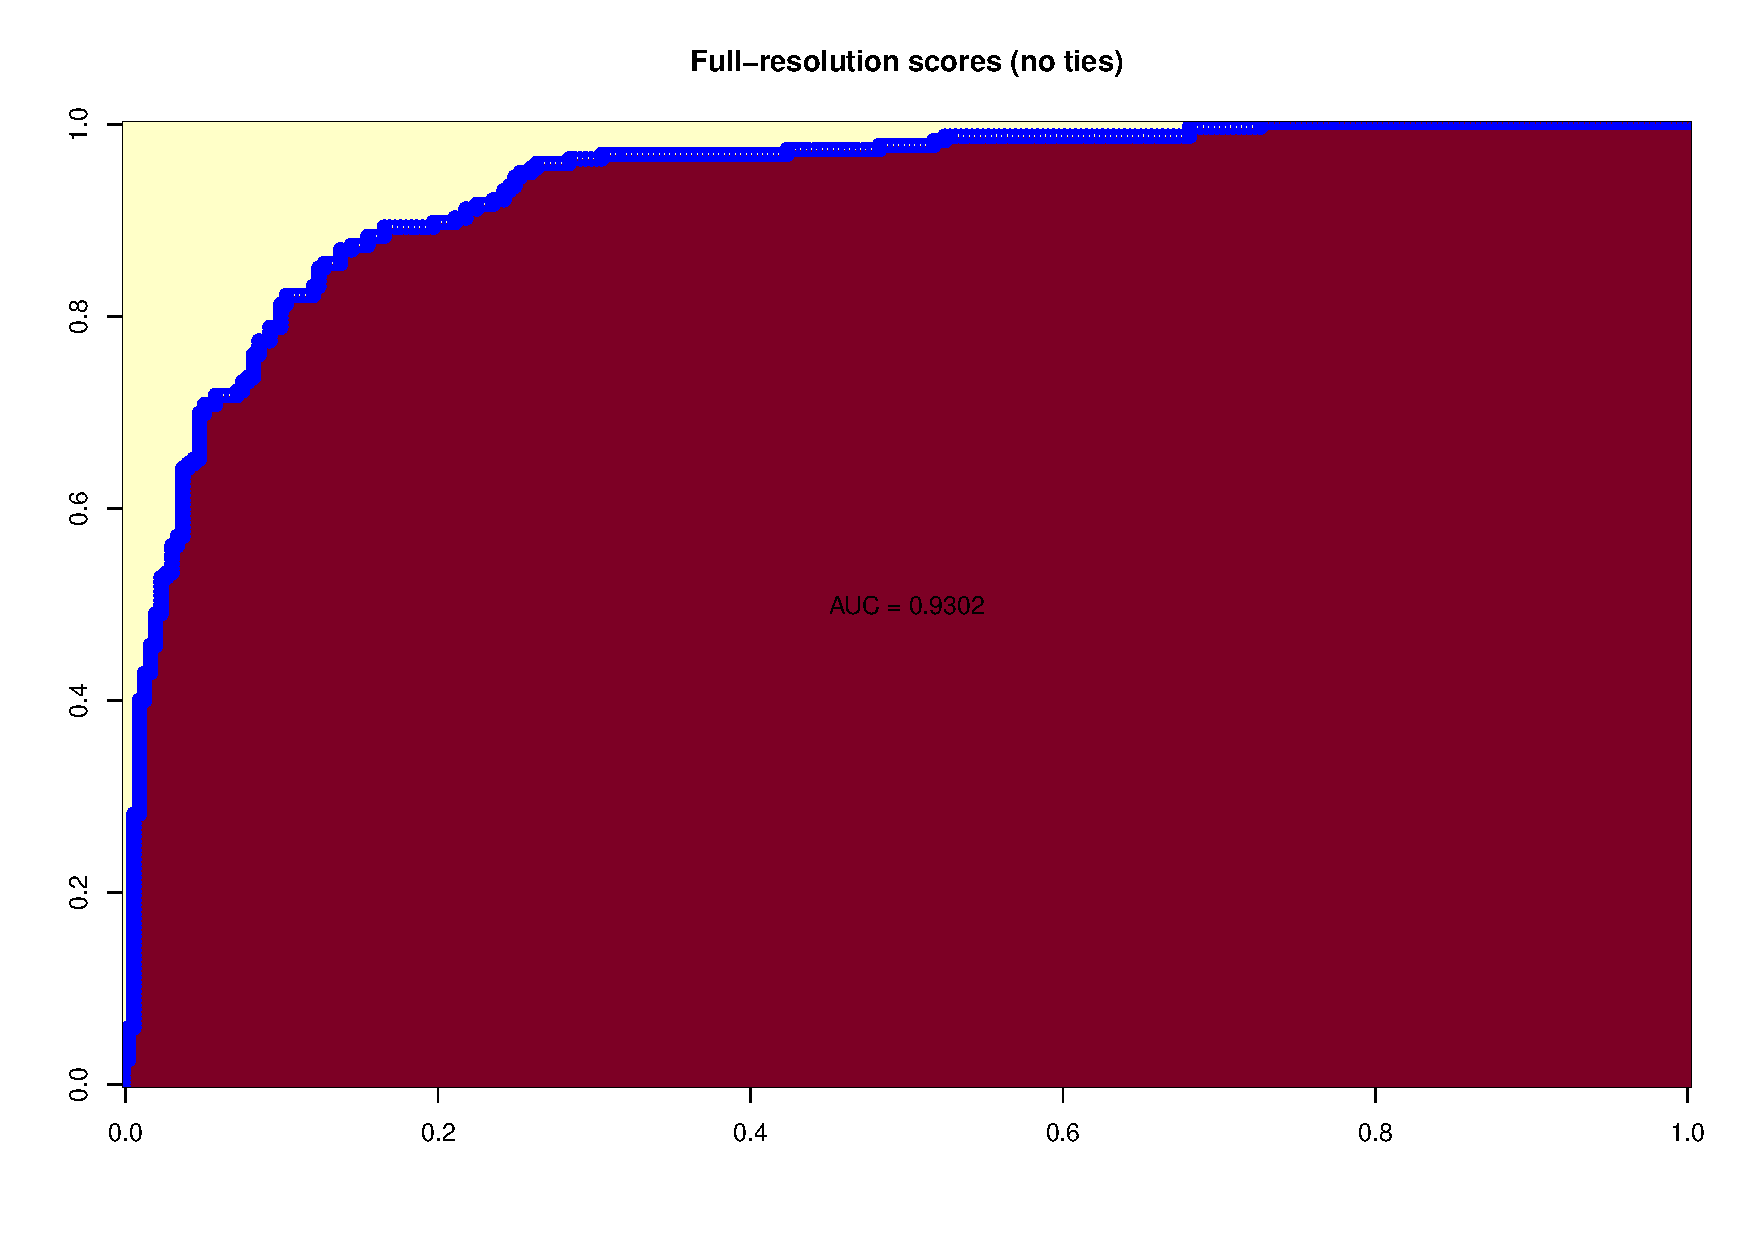
\includegraphics[width=0.95\textwidth]{full-res-scores-no-ties-r.pdf}
	\caption{ROC curve for the original defective parts data based on the comparison matrix.}
	\label{fig:bad-parts-ROC-original-r}
\end{figure}
%
\begin{figure}[htp]
	\centering
	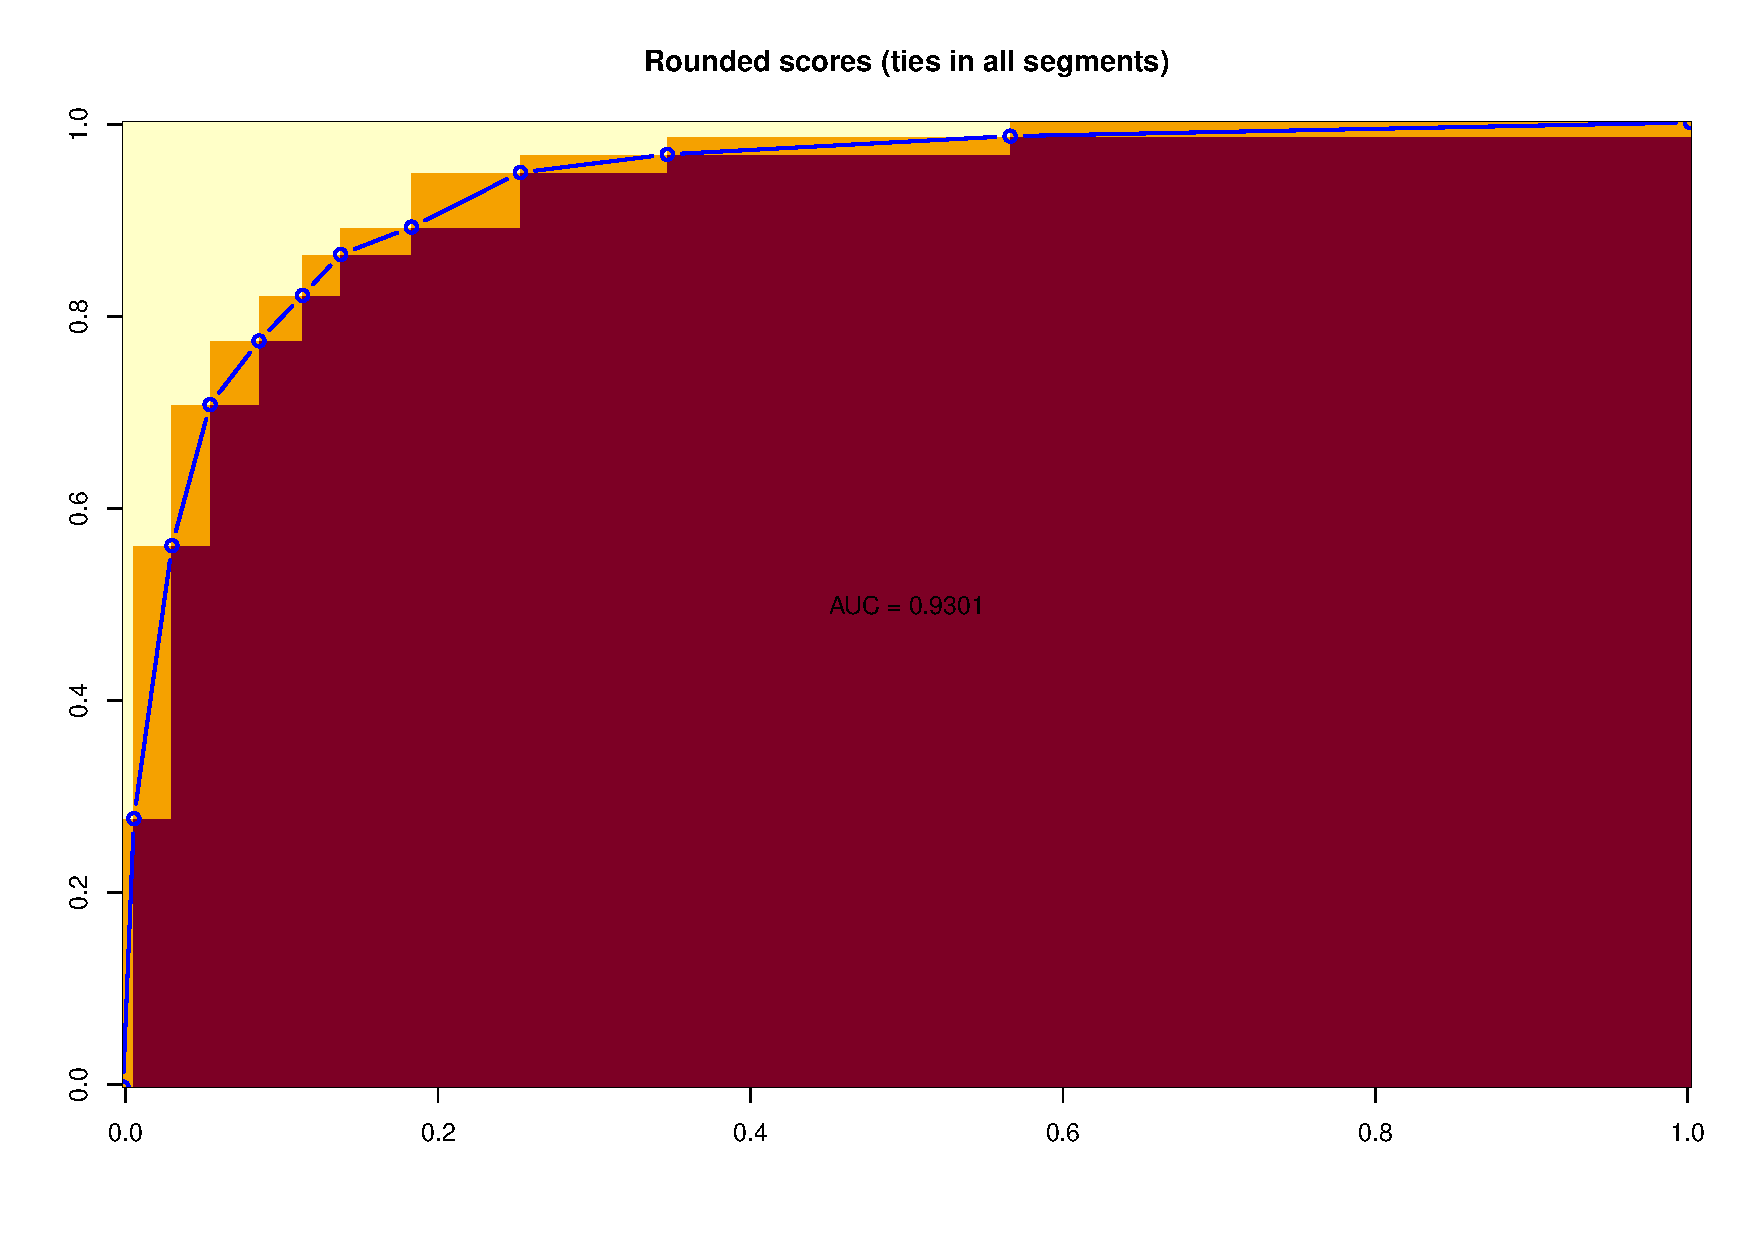
\includegraphics[width=0.95\textwidth]{rounded-scores-all-ties-r.pdf}
	\caption{ROC curve for the rounded defective parts data based on the comparison matrix.}
	\label{fig:bad-parts-ROC-rounded-r}
\end{figure}
%

Diagram~\ref{fig:bad-parts-ROC-original-r} contains the ROC-curve based on the original data. Diagram~\ref{fig:bad-parts-ROC-rounded-r} contains the ROC curve based on rounded scores. As you can see, each section is a~diagonal segment running to the "North-East". It was shown earlier that this direction corresponds to repeated values.

The final results of the AUC calculations by the four methods are shown in Table~\ref{tab:calc-AUC-4-methods-r}. As can be seen, all three of our own functions calculate the AUC quite well.  They give close results with respect to the result of the function from the package \textbf{pROC}. Naturally, these self-made functions serve more for training purposes. In practice, you should use the standard tools, such as \textbf{pROC} or \textbf{ROCR}.
%

\begin{table}[ht]
	\caption{Results of AUC calculation by four methods.}\label{tab:calc-AUC-4-methods-r}
	\centering
	\begin{tabular}{lll}
		\hline
		& Full.Resolution & Rounded.Scores \\ 
		\hline
		auc & 0.9302279874213836841079 & 0.9301379061844864404307 \\ 
		appraiser\_auc & 0.9302279874213836841079 & 0.9301379061844863294084 \\ 
		rank\_comparison\_auc & 0.9302279874213835730856 & 0.9301379061844864404307 \\ 
		auc\_probability & 0.9307199999999999917577 & 0.9291749999999999731770 \\ 
		\hline
	\end{tabular}
\end{table}
%
\subsubsection{Summary of AUC findings}
The analysis of the concept of AUC was carried out in the previous sections. The algorithms for calculating its value, including those based on the probabilistic approach, were also presented. In general, it can~be said that an in-depth study of issues related to ROC and AUC is not strictly necessary for the successful application of the U-test in the practical work of the appraiser. While the geometric approach to calculating the AUC is still quite intuitive and simple, interpreting the AUC as a~probability seems somewhat abstruse and requires a~certain level of general mathematical background.

However, in the context of valuation activities, the concept of AUC as a~probability is indeed quite useful. Appraisers often deal with relatively small samples. In this case, they need to understand the extent to which they can~be confident that the value of the object that has some of the features exceeds the value of the object that does not have it (or vice versa). Thus, the use of the AUC refers us to the Bayesian approach to probability, which includes the concept of \emph{level of certainty}. This draws a bridge between traditional frequentist statistics, within the framework of which the U-test was once developed, and modern machine learning, based for the most part on a Bayesian approach to probability. In the author's opinion, this circumstance alone is sufficient reason to delve into the topics of ROC and AUC when examining the practical issues of using the U-test by appraisers.

In addition, the objectives of appraisers are not limited only to determining the value itself. The use of classifiers can often have independent utility at an earlier stage of the valuation process, for example, at the stage of determining the properties of the objects being valued. The general behavior of the classifier over the entire range of possible threshold values is quite often of less interest than its behavior in a~certain relatively narrow range. For example, when solving the above discussed problem of separating defective parts from quality parts, the performance of the classifier in the boundary zone of threshold values is crucial. In this case, the specific setting of such a threshold value may depend on the purpose of the valuation. For example, from the point of view of the lending bank or the Central Bank, which monitors the adequacy of collateral, the sensitivity of the classifier is in a~sense more important than its specificity, because the assignment of defective parts to quality parts carries more risk than the reverse situation. At the same time, from the point of view of, for example, the tax inspection, classifying serviceable assets as faulty with their subsequent write-off from the balance sheet of the enterprise, leading to a decrease in the taxable base, is a~more serious problem than the erroneous attribution of faulty to serviceable, i.\,e. a~situation arises where specificity is more important than sensitivity. Thus, there may~be situations where the cost of Type~I and Type~II errors is not the same. Such situations present a~definite problem because the AUC concept assumes the same cost of these errors. However, this topic is quite specific and goes beyond the scope of this material, the topic of which is the U-test. Briefly, we can say that there are metrics other than AUC to account for the different cost of Type I and Type II errors. For further study of the topic of AUC on your own, we can recommend \href{http://nicolas.kruchten.com/content/2016/01/ml-meets-economics/}{this material}~\cite{ML-meets-economics}.
%
\chapter{Practical implementation}\label{U-test-practice}
%
\section{Implementation in the LibreOffice Calc spreadsheet}\label{U-test-spreadsheet}
At this point, it is safe to say that spreadsheets are the standard tool for appraisers' calculations. Introducing development tools such as Python and R~programming languages into professional activities is quite slow. In addition, an independent step-by-step calculation allows for a better understanding of the U-test methodology. Therefore, it was decided to create a step-by-step instruction for the U-test in a spreadsheet. The software product LibreOffice Calc (Version: 7.3.5.2 / LibreOffice Community
Build ID: 30(Build:2) CPU threads: 4; OS: Linux 5.11; UI render: default; VCL: kf5 (cairo+xcb)
Locale: en-US (en\_US.UTF-8); UI: en-US Ubuntu package version: 1:7.3.5~rc2-0ubuntu0.20.04.1~lo1
Calc: threaded) was used for this purpose. A significant part of its functionality is also available in the most common application of this kind, Microsoft Excel. There is no reason to believe that the calculations made will not work correctly in applications other than LibreOffice Calc. However, it is also impossible to guarantee this. For an unambiguously correct test it is recommended to use this application, which has versions for all major operating systems. In addition, the use of free software is generally good practice. The current version of the spreadsheet~\href{https://github.com/Kirill-Murashev/AI_for_valuers_book/blob/main/Parts-Chapters/Mann-Whitney-Wilcoxon/U-test.ods}{U-test.ods} is in the ~\href{https://github.com/Kirill-Murashev/AI_for_valuers_book/tree/main/Parts&Chapters/Mann-Whitney-Wilcoxon}{repository} along with the rest of this work.

The data considered in this section are fictitious and were generated by the LibreOffice Calc pseudorandom number generation algorithm. To re-generate, use the key combination \emph{ctrl+shift+F9}.

Consider the training task. Cells I3:J30 contain data of values of some quantitative feature for observations of two samples taken from sets~\textit{I} and~\textit{J}, respectively. The difference between the elements of these sets is the presence of some attribute in the set \textit{I} and its absence in the set \textit{J}. The task is to test the hypothesis that the difference in a given attribute should be recognized as significant, and the attribute itself is a pricing factor. Let us create the null-hypothesis by formulating it in three variants corresponding to the three levels of rigor described earlier in Table~\ref{tab:nul-hypothesis-variants}. It should be noted that the U-test refers to statistics based on the so-called frequentist approach to probability. For a discussion of the differences between the \emph{frequentist} and \emph{Bayesian} approaches to probability as applied to value estimation, see, in particular~\cite{Murashev:freq-baye-prob}. As you know, the \emph{frequentist} approach is based on the premise that randomness is a consequence of objective uncertainty, which can only be reduced by a series of experiments. In the frequentist approach there is a clear division into random and non-random parameters. A typical task is to estimate certain parameters of the general population, which is a set of random variables. For this purpose, deterministic sampling parameters such as mean, mode, variance, etc. are used. The latter represent specific values in which there is no longer any randomness. Thus, we initially accept the fundamental assumption of the random nature of the variables under study. Then we apply some methods of mathematical statistics, which allow us to obtain specific values of parameter estimates. This allows us to reduce the level of uncertainty, which nevertheless always remains. It follows that the null hypothesis is most often pessimistic. It carries the assertion that the phenomenon or process under study is based on chance, so that we are unable to draw reliable conclusions. In contrast, the alternative hypothesis says that the level of uncertainty can be reduced due to the success of the experiment. Considering all of the above, let us formulate the null and alternative hypotheses in three variants according to different levels of rigor and record them in Table~\ref{tab:nul-alt-hypothesis-variants}.
%
\begin{table}[htp]
	\caption{The null hypothesis and the alternative hypothesis in the analysis of training data.}  \label{tab:nul-alt-hypothesis-variants}
	\centering
	\begin{tabularx}{\textwidth}{p{0.15\linewidth} p{0.4\linewidth} p{0.4\linewidth}} 
		\hline
		Type of hypothesis&The null hypothesis (H0)&The alternative hypothesis (H1)\\
		\hline
		Scientific&The distribution of the specific value indicators is the same for the analogues with attribute \textit{"X"} (set of objects \textit{I}) and without it (set of objects \textit{J}). There is no bias between them, the statistical estimates made for one set of objects are unbiased for the other set.&The distribution of unit values for objects from set \textit{I} differs from the distribution that occurs in set \textit{J}. There is a bias, the estimate made for objects belonging to one set will be biased for objects belonging to another set.\\
		\hline
		Practical&The median value of the unit value of objects with attribute \textit{"X"} does not differ from the median value of the unit value of objects without attribute \textit{"X"}, their medians are equal.&The median value of the unit value of objects with attribute \textit{"X"} differs from the median value of the unit value of objects without attribute \textit{"X"}, their medians are not equal.\\
		\hline
		Set forth in terms of valuation&The presence or absence of an attribute  \textit{"X"} does not have any noticeable effect on the value, so the attribute \textit{"X"} is not a pricing factor.&The presence or absence of an attribute \textit{"X"} has a noticeable effect on the value, therefore, the attribute \textit{"X"} is a pricing factor.\\ \hline
	\end{tabularx}
\end{table}
%
Cells C2:C19 contain some descriptive statistics. It can be useful to show the properties of samples graphically for ease of primary analysis. Figure~5 shows a Boxplot diagram that allows us to draw some conclusions based on one glance. As can be seen, the values of the means and medians of the two samples are different. The minimum values also vary. At the same time, the maximum values are the same. It should also be noted that although the mean and median of the first sample are higher than those of the second, the minimum value of the first is lower than that of the second. In such circumstances, it is even more difficult to conclude whether the difference in the attribute is significant, or whether the difference in the unit value indicator is incidental in nature.
%
\begin{figure}[htp]
	\centering
	\includegraphics[width=0.95\textwidth]{BoxPlot.pdf}
	\caption{Boxplot for both samples.}
	\label{fig:BoxPlot}
\end{figure}
%
The next preparatory step is to check the normality of the distribution of values of the quantitative attribute (in this case, the notional unit cost). There are a number of rigorous tests that allow such testing by numerical methods. Appropriate ways of performing such tests will be shown in sections~\ref{U-test-Python} and~\ref{U-test-R}. We only use the graphical method in this section. Histograms of probability density distributions for the first and second samples are shown in Figures~\ref{fig:s1-hist} and~\ref{fig:s2-hist}, respectively. They are combined with the curves of the probability density function for the normal distribution.
%
\begin{figure}[htp]
	\centering
	\includegraphics[width=0.95\textwidth]{s1-hist.pdf}
	\caption{Histogram of the first sample, combined with the curve of the probability density function for the normal distribution.}
	\label{fig:s1-hist}
\end{figure}
%
\begin{figure}[htp]
	\centering
	\includegraphics[width=0.95\textwidth]{s2-hist.pdf}
	\caption{Histogram of the second sample, combined with the curve of the probability density function for the normal distribution.}
	\label{fig:s2-hist}
\end{figure}
%

The shape of the distribution of both samples differs significantly from the shape of the curve of the probability density function of the normal distribution, which can be clearly seen in the diagrams~\ref{U-test-Python}, \ref{U-test-R}.When working with real data, quantitative tests for normality of distributions must be performed in all cases. Let us focus on the interpretation of the diagrams in this section. The shape of both histograms allows us to conclude that the distributions of both samples differ from normal. This allows us to conclude that parametric methods of statistical estimation are not applicable. It is necessary to use methods of non parametric statistics, which include the U-test, in such a situation.

There is no need to construct a common variation series for two samples when working with a spreadsheet. You can go straight to the calculation of the observation ranks through the standard LibreOffice Calc tools. Considering the possible presence of ties (repeating values) you should use the \texttt{RANK.AVG} function. The three arguments for it to work correctly must be specified consistently:
\begin{itemize}
	\item the observation for which the rank is calculated;
	\item the range of all values of the common variation series;
	\item sorting type: 0 --- descending, 1 --- ascending, in our case it is necessary to specify~1.
\end{itemize}
Columns~\textit{M} and~\textit{O} contain the ranks of the corresponding observations. Columns~\textit{L} and~\textit{N} contain duplicate values.

After that, in cells C20:C21 we calculate the sums of ranks for each of the samples. After that, calculate the total sum of the ranks of both samples in cell C22. Let's calculate the same indicator according to formula~\ref{eq:common-R} for verification.

Next, in cells C25, C26 we calculate the values of U1 and U2 according to formulas~\ref{eq:U1}, \ref{eq:U2}, respectively. Then in cell D27 we check the correctness of the control ratio~\ref{eq:check-U-value}. In C28 we select a smaller value, which will be used later as the U-statistic. In our case, the sample from set~J has a smaller U-statistic value.

Let's calculate the CLES indicator. To do this we use formula~\ref{eq:CLES}. The result is found in~C29. In this example, the value of the indicator is~0.61. This should be interpreted as follows: \emph{the probability that the value of the unit value of a randomly chosen observation from set I is greater than that of a randomly chosen observation from set J is 0.61~(61\%)}. Next, we calculate the value of the rank-biserial correlation coefficient by formulas~\ref{eq:RBC-formula-1}, \ref{eq:RBC-formula-2}. Put it in cell~C36. In this case, the value was 0.21. So the strength of the correlation between the presence of the attribute \textit{"X"} and the unit value of the object is~0.21.

After that, we proceed to calculate the standardized value (z-score) by formula~\ref{eq:z-score}. To do this in cell C38, calculate the mean using formula~\ref{eq:U-mean}. Then we move on to the question of calculating the standard deviation. It should be noted that there are two formulas for this. The first~(\ref{eq:standard-deviation-no-ties}) applies if there are no ties (cell C39). The second~(\ref{eq:standard-deviation-ties}) applies when they are present (cell C40). In the case at hand, ties were present. They were processed in columns~P and~Q, as well as in cells~E35:E49. In this paper, both formulas were applied. The result was two values with a difference of less than one percent. Consideration of the ties factor is necessary from the point of view of maximum scientific correctness of the result. However, some appraisers in their daily practice may find it difficult to correctly account for the bundling factor. Or they may not have enough time for additional calculations. Practical experience tells us that any significant difference in the standard deviation values obtained using these two formulas occurs in cases of a large number of ties or the presence of large groups. In other situations, a simpler formula that automatically calculates the~${\sigma}$ value gives the correct result. Its accuracy for valuation is quite sufficient. In any case, the decision to use more scientific and rigorous or simple methods is up to the appraiser. The ties factor has been taken into account in the example under consideration. Knowing the mean and standard deviation, we calculate the z-score in cell C45. The continuity of the distribution is one of the prerequisites of the U-test. However, the empirical data are discrete. Therefore, the implementation of the adjustment by subtracting~0.5 is necessary. Then in cell C46 we calculate the p-value by approximating the normal distribution. In this example it was~0.173. According to the rule~\ref{eq:p-interpretation}, we conclude that it is impossible to reject the null hypothesis. Using the wording closest to the valuation activity (see Table~\ref{tab:nul-alt-hypothesis-variants}), we can come to the following conclusion: the presence or absence of attribute~"X" does not have any noticeable effect on the value, attribute~"X" is not a pricing factor.

In this section, we looked at the step-by-step calculation of the criterion statistics, as well as carried out the interpretation of the result. As shown above, conducting the U-test in a spreadsheet is quite convenient. However, it is difficult to consider as a best practice. Preference should be given to professional development tools in machine learning and statistical inference. Python and R programming languages are such tools in the first place.
%
\clearpage
%
\section{Python implementation.}\label{U-test-Python}
%
\lstset{language=Python,
	basicstyle=\ttfamily,
	keywordstyle=\color{Blue}\ttfamily,
	stringstyle=\color{Red}\ttfamily,
	commentstyle=\color{Emerald}\ttfamily,
	morecomment=[l][\color{Magenta}]{\#},
	breaklines=true,
	breakindent=0pt,
	breakatwhitespace,
	columns=fullflexible,
	showstringspaces=false
}
%
Python language has already become the de facto standard in machine learning and especially in a number of areas such as deep learning. In addition, it is versatile and perfectly suited for the development of various expert systems.  Its popularity means, among other things, that there are a huge number of tutorials on all aspects of development in the field of data analysis, designed for users of any level of training. Most of the calculations required by the appraiser can be done by calling standard functions from the data analysis plug-in libraries. These include, but are not limited to: \textbf{TensorFlow}, \textbf{NumPy}, \textbf{SciPy}, \textbf{Pandas}, \textbf{Matplotlib}, \textbf{Keras}, \textbf{SciKit-Learn}, \textbf{PyTorch}, \textbf{Scrapy}, \textbf{BeautifulSoup}. There is no need to write a large amount of code in this case. You don't need to have a deep knowledge of programming either. According to the author of this paper, the future of valuation lies precisely in the implementation of expert systems based on learning models from open market datasets. The use of Python significantly reduces the time of the U-test as will be shown below. It also allows you to create visualizations of market data without resorting to third-party tools. In addition, the use of professional functions virtually eliminates the possibility of errors in calculations. The Python language version 3.9.12 was used when writing the code. The Python language version 3.9.12 was used when writing the code. The author used the Spyder IDE (version 5.1.5) and the Jupyter Lab development environment (version 3.3.2). Python scripts containing the used code are available in the~\href{https://github.com/Kirill-Murashev/AI_for_valuers_Python_source/tree/main/Mann-Whitney-u-test}{repository}~\cite{Murashev:U-test.py}, ~\cite{Murashev:U-test.ipynb}.

Let us consider a real data set containing information on the unit cost of apartments in the St.~Petersburg agglomeration. The data were scraped on September 28, 2021 from \href{https://www.cian.ru/}{cian.ru} and are available at~\href{https://github.com/Kirill-Murashev/datasets/blob/main/Saint-Petersburg/flats/spba_flats_210928.csv}{the link}~\cite{ds:spba-flats-210928}. The dataset under consideration contains 34821 observations. As you know, the St.~Petersburg agglomeration includes territories that are part of the Federal City, as well as those that are formally part of the Leningrad Region (Leningrad Oblast). The division into city and region is of a purely legal nature. From a socio-economic point of view, the nearest territories of the Leningrad Region are inextricably linked to St.~Petersburg and are part of one agglomeration. By the way, it is the largest in the world at this latitude. When forming the queries used in the scraping process, the southern boundary of the agglomeration was established approximately along the axis of the A-120 highway, while the northern boundary was established along the 41A-189 highway. At the same time, it included some settlements outside these boundaries, such as the cities of Kirovsk and Schlisselburg.

Let us formulate the problem. It is necessary to determine whether or not there is a statistically significant difference in the prices of objects located within the boundaries of St.~Petersburg and objects formally located in the Leningrad region. Similarly to the previous case, let us formulate the null and alternative hypotheses, which this time make practical sense (see Table~\ref{tab:nul-alt-hypothesis-SPba}).
\begin{table}[htp]
	\caption{The null and alternative hypotheses in the analysis of data from the St.~Petersburg urban agglomeration}\label{tab:nul-alt-hypothesis-SPba}
	\centering
	\begin{tabularx}{\textwidth}{p{0.15\linewidth} p{0.4\linewidth} p{0.4\linewidth}} 
		\hline
		Type of hypothesis&The null hypothesis (H0)&The alternative hypothesis (H1)\\
		\hline
		Scientific&The distribution of unit cost indicators for apartments located within the borders of St.~Petersburg and apartments located in the adjacent areas of the Leningrad Region is the same. There is no shift between the two. The statistical estimates made for the set of analogues located in one part of the agglomeration are unbiased for objects located in the other part.&The distribution of unit cost indicators for apartments located within the borders of St.~Petersburg differs from the distribution of unit cost indicators for apartments located in the adjacent territories of the Leningrad Region. There is a shift. The estimate made for objects located in one part of the agglomeration will be biased for objects located in another part of it.\\
		\hline
		Practical&The median of the unit value of apartments located within the borders of St.~Petersburg is equal to the median of the unit value of apartments located in the adjacent territories of the Leningrad Region.&The median of the unit value of apartments located within the borders of St.~Petersburg is not equal to the median of the unit value of apartments located in the adjacent territories of the Leningrad Region.\\
		\hline
		Set forth in terms of valuation&The location of the apartment within the borders of St.~Petersburg or in the adjoining areas of the Leningrad Region is not a significant difference and does not require any special accounting.&The location of the apartment within the borders of St.~Petersburg or in the surrounding areas of the Leningrad Region is a significant difference and requires separate accounting.\\ \hline
	\end{tabularx}
\end{table}

The Python language was not originally designed specifically for data analysis. Therefore, many of the functions required for calculations will be missing in its basic version. Fortunately, there are a number of libraries that contain many necessary functions. Their number is not as large as, for example, in the R language. Their functionality is also somewhat less than that of the R. However, they are exhaustive for the overwhelming number of tasks facing appraisers. We need the following libraries: \textbf{numpy}, \textbf{pandas},\textbf{ math}, \textbf{matplotlib.pyplot}, \textbf{scipy.stats} to solve the problems discussed in this paper. Use the code provided in script~\ref{lst:import-libraries-Python} to enable them.
\begin{lstlisting}[float=htp, caption = Enabling the required libraries, firstnumber=1, label= lst:import-libraries-Python]
# import libraries
import numpy as np
import pandas as pd
import math
import matplotlib.pyplot as plt
import scipy.stats as stats
from scipy.stats import norm
from scipy.stats import normaltest
from scipy.stats import shapiro
from scipy.stats import anderson
from scipy.stats import mannwhitneyu
\end{lstlisting}
%

Let us set the significance level $\alpha$, which is adopted for all further work. The choice of its value is the appraiser's prerogative. However, the most common value in papers on econometrics and operations research is~0.05. Code~\ref{lst:set-alpha} was used to set the significance level value.
%
\begin{lstlisting}[float=htp, caption = Set the applicable level of significance, firstnumber=1, label= lst:set-alpha]
# set significance level
alpha = 0.05
\end{lstlisting}
% 

Now everything is ready to get to work. Let's create a dataframe based on the text file containing the data set under analysis (see script~\ref{lst:import-data-create-dataframe}).
%
\begin{lstlisting}[float=htp, caption = , firstnumber=1, label= lst:import-data-create-dataframe]
# import dataset
df = pd.read_csv('spba-flats-210928.csv')
print(df)
type(df['price_m'])
\end{lstlisting}
%
The dataframe repeats the contents of the original file exactly and contains 34821 observations and 4 variables. The following variables are present.
\begin{itemize}
	\item Number.
	\item Link to ad.
	\item Price per 1\,sq.~m.
	\item A six-letter location code:
	\begin{itemize}
		\item the first of which indicates the region (s --- St.~Petersburg, l --- Leningrad Region);
		\item the second and third indicates the administrative district;
		\item the last three indicate the municipality or territory.		
	\end{itemize}
\end{itemize}
Python added its own variable containing the observation numbers. That makes five variables. Note that numbering in Python begins with zero, not one, as in most programming languages. Variables containing observation numbers and links to ads from the source file will not be used further. So we will create a new dataframe containing only the necessary variables. Let's also release the virtual memory by unloading the first dataframe from it to optimize the computer's resources. See script~\ref{lst:create-new-dataframe-release-RAM}. Such micro-optimization does not play a role in the case at hand. However, in order to learn how to create good code, it is better to write one extra line.
%
\begin{lstlisting}[float=htp, caption = Creating a dataframe containing only necessary variables and freeing memory from objects not used later, firstnumber=1, label= lst:create-new-dataframe-release-RAM]
# get only prices and counties, release RAM
df1 = df[['price_m', 'county']]
del [[df]]
\end{lstlisting}
%

The appraiser now has at his disposal a working dataframe in a convenient form. It contains data on the apartment market of the entire St.~Petersburg agglomeration. Let's plot a histogram combined with the density curve for the normal distribution to form the first view about the distribution. The Heinhold-Gaede formula ~\cite{Ingenieur-Statistik} was used to determine the rational number of intervals (histogram columns) --- \textit{k}.
\begin{equation}\label{eq:k-hist-Heinhold-Gaede}
k = \sqrt{n},
\end{equation}
where~\textit{n} --- is the number of observations. ~\ref{lst:price-hist-spba}. Script~\ref{lst:price-hist-spba} was used to plot the histogram.
%
\begin{lstlisting}[float=htp, caption = Plotting the histogram for the agglomeration of St.~Petersburg., firstnumber=1, label= lst:price-hist-spba]
# calculate the number of observations on data frame
spbaLenR = round(math.sqrt(len(df1.index)))

# fit a normal distribution to the data: mean and standard deviation
mu, std = norm.fit(df1["price_m"])

# plot the histogram
plt.hist(df1["price_m"], bins=spbaLenR, density=True)

# plot the PDF
xmin, xmax = plt.xlim()
x = np.linspace(xmin, xmax, 100)
p = norm.pdf(x, mu, std)

plt.plot(x, p, 'k', linewidth=2)
title = "Fit Values: {:.2f} and {:.2f}".format(mu, std)
plt.title(title)

# save to .pdf
plt.savefig('spba-price-histogram-py.pdf')
\end{lstlisting}
%

Consider the resulting histogram~\ref{fig:spba-prices-hist}. The x-axis contains the values of prices per square meter, the y-axis the values of the probabilities of intervals. Both axes are presented in standard form. The expectation and standard deviation values for the theoretical normal distribution are also shown. As you can see, the distribution has a heavy right tail. This allows us to draw a preliminary conclusion that it is different from normal. Formalized normality tests will be performed in the future. We can limit ourselves to the primary subjective interpretation of the histogram for now.
%
\begin{figure}[htp]
	\centering
	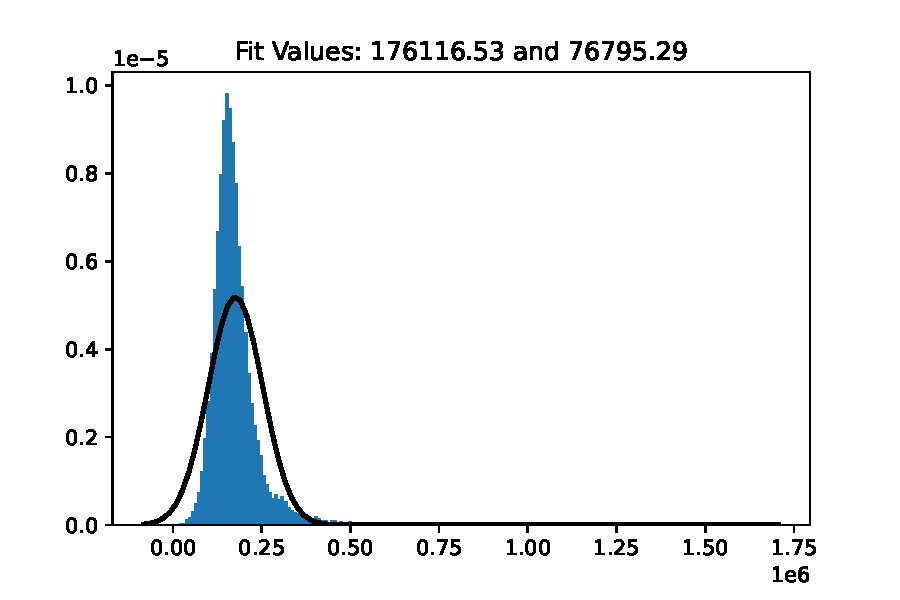
\includegraphics[width=0.95\textwidth]{spba-price-histogram-py.pdf}
	\caption{Histogram of the density distribution of apartments' prices per 1~sq.\,m. in agglomeration of  St.~Petersburg combined with the curve of the probability density function for the normal distribution.}
	\label{fig:spba-prices-hist}
\end{figure}
%
The subject of the research is the difference between the objects located in the two parts of the agglomeration. The initial dataset contains information about observations from both parts. Therefore, it will be necessary to create two separate dataframes.A small digression should be made here. Practical experience tells us that data analysis itself and model development take less than 20\,\% of the time, while more than 80\,\% is spent on data collection and preprocessing. Correct data markup is one of the important elements of these processes. In the case of the data set under consideration, their analysis in terms of individual territories up to the level of municipalities was initially provided by specifying a territory index for each observation. The first letter of the index contains an indication of which part of the agglomeration the observation is located in, as mentioned above. Two lines of code (see script~\ref{lst:create-two-separate-df-for-S-Pb-LO}) containing simple regular expressions are enough to create two separate dataframes in this case.
%
\begin{lstlisting}[float=htp, caption = Creating separate dataframes for St.~Petersburg and the Leningrad Region., firstnumber=1, label= lst:create-two-separate-df-for-S-Pb-LO]
# create separate dataframes for city and suburbs
dfs = df1[df1['county'].str.startswith('s')] # Saint-Petersburg
dfl = df1[df1['county'].str.startswith('l')] # Leningradskaja oblastq
\end{lstlisting}
%
The \emph{dfs} dataframe contains data for observations from St.~Petersburg (28643 observations). The \emph{dfl} dataframe contains data for observations from the Leningrad Region (6178 observations). Let's plot the histograms for both parts of the agglomeration. See scripts ~\ref{lst:price-hist-spb} and \ref{lst:price-hist-lo}.
%
\begin{lstlisting}[float=htp, caption = Histogram plotting for St.~Petersburg., firstnumber=1, label= lst:price-hist-spb]
# Saint-Petersburg
# calculate the number of observations on data frame
spbLenR = round(math.sqrt(len(dfs.index)))

# fit a normal distribution to the data: mean and standard deviation
muS, stdS = norm.fit(dfs["price_m"])

# plot the histogram
plt.hist(dfs["price_m"], bins=spbLenR, density=True)

# plot the PDF
xmin, xmax = plt.xlim()
x = np.linspace(xmin, xmax, 100)
ps = norm.pdf(x, muS, stdS)

plt.plot(x, ps, 'k', linewidth=2)
title = "S-Pb. Fit Values: {:.2f} and {:.2f}".format(muS, stdS)
plt.title(title)

# save to .pdf
plt.savefig('spb-price-histogram-py.pdf')
\end{lstlisting}
%
\begin{lstlisting}[float=htp, caption = Histogram plotting for the Leningrad Region, firstnumber=1, label= lst:price-hist-lo]
# LO
# calculate the number of observations on data frame
loLenR = round(math.sqrt(len(dfl.index)))

# fit a normal distribution to the data: mean and standard deviation
muL, stdL = norm.fit(dfl["price_m"])

# plot the histogram
plt.hist(dfl["price_m"], bins=loLenR, density=True)

# plot the PDF
xmin, xmax = plt.xlim()
x = np.linspace(xmin, xmax, 100)
pl = norm.pdf(x, muL, stdL)

plt.plot(x, pl, 'k', linewidth=2)
title = "LO. Fit Values: {:.2f} and {:.2f}".format(muL, stdL)
plt.title(title)

# save to .pdf
plt.savefig('lo-price-histogram-py.pdf')
\end{lstlisting} 
%
\begin{figure}[htp]
	\centering
	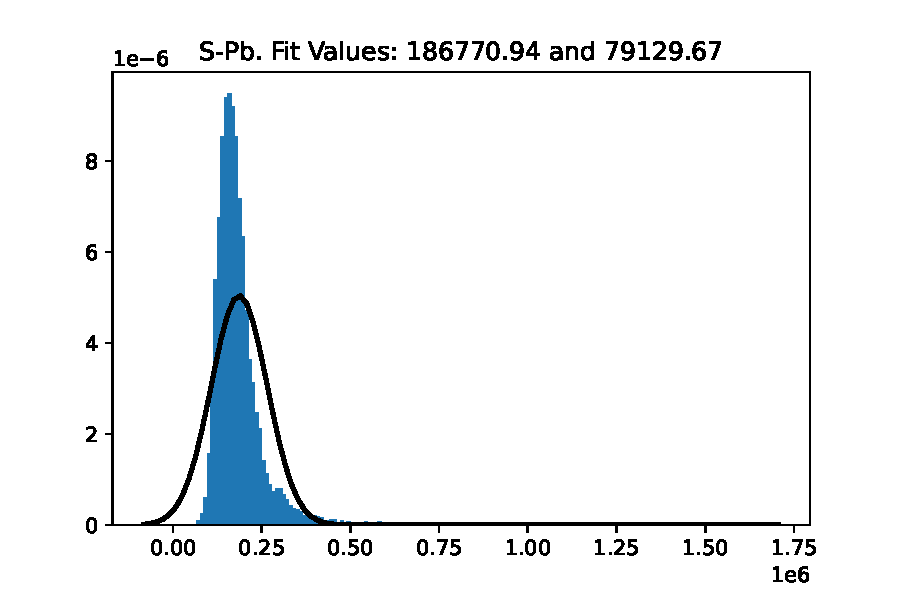
\includegraphics[width=0.95\textwidth]{spb-price-histogram-py.pdf}
	\caption{Histogram of the density distribution of apartments' prices per 1~sq.\,m. in St.~Petersburg combined with the curve of the probability density function for the normal distribution.}
	\label{fig:spb-prices-hist}
\end{figure}
%
\begin{figure}[htp]
	\centering
	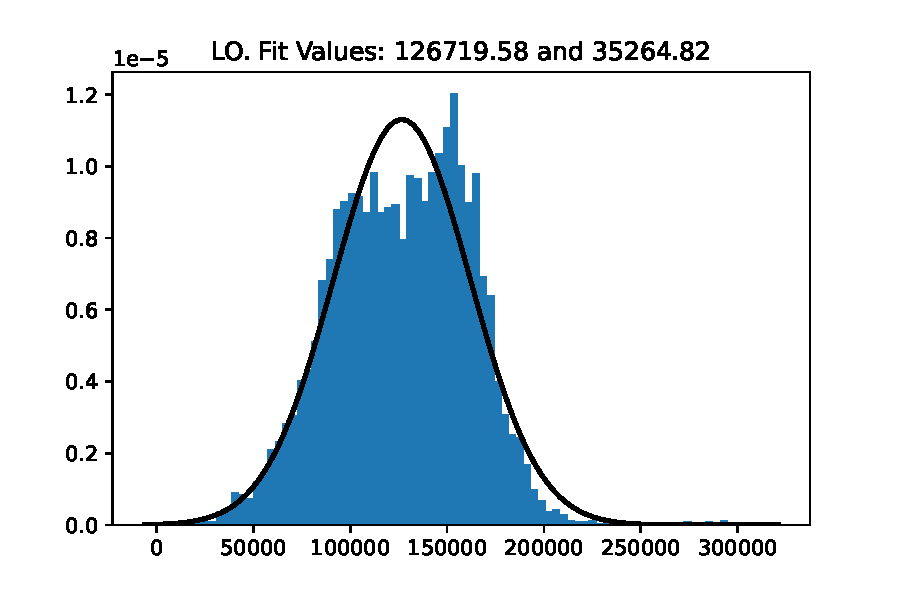
\includegraphics[width=0.95\textwidth]{lo-price-histogram-py.pdf}
	\caption{Histogram of the density distribution of apartments' prices per 1~sq.\,m. in the Leningrad Region located within the borders of the St.~Petersburg agglomeration combined with the curve of the probability density function for the normal distribution.}
	\label{fig:lo-prices-hist}
\end{figure}
%

The histogram is sometimes confused with the bar graph. Recall that a properly plotted histogram is a representation of the probabilistic properties of the data. The sum of the areas of all its rectangles must be equal to one. Therefore, the probability values of the ranges (histogram columns), rather than the number of observations in each range, must be plotted on the y-axis. As can be seen in histogram~\ref{fig:spb-prices-hist}, the distribution of unit prices in St.~Petersburg as well as in the case with the distribution of prices for the entire agglomeration has a heavy right tail. In contrast, the distribution of prices for the agglomeration objects located outside the boundaries of St.~Petersburg, shown in histogram~\ref{fig:lo-prices-hist}, looks relatively symmetrical.

Let's also plot the boxplot for both dataframes using script~\ref{lst:boxplot-spba}. As can be seen in Diagram~\ref{fig:spb-lo-boxplot-py}, the value of median unit prices of properties located in St.~Petersburg is higher than the value of the third quartile of prices of properties located in the adjacent areas of the Leningrad Region.
%
\begin{lstlisting}[float=htp, caption = Plotting the boxplot for both subsamples, firstnumber=1, label= lst:boxplot-spba]
# add labels to data
dfs["region"] = "SPb"
dfl["region"] = "LO"

# plot boxplot
prices = [dfs, dfl]
allPrices = pd.concat(prices)
plt.figure()
allPrices.boxplot(by="region")

# save to .pdf
plt.savefig('spb-lo-boxplot-py.pdf')
\end{lstlisting} 
%
\begin{figure}[htp]
	\centering
	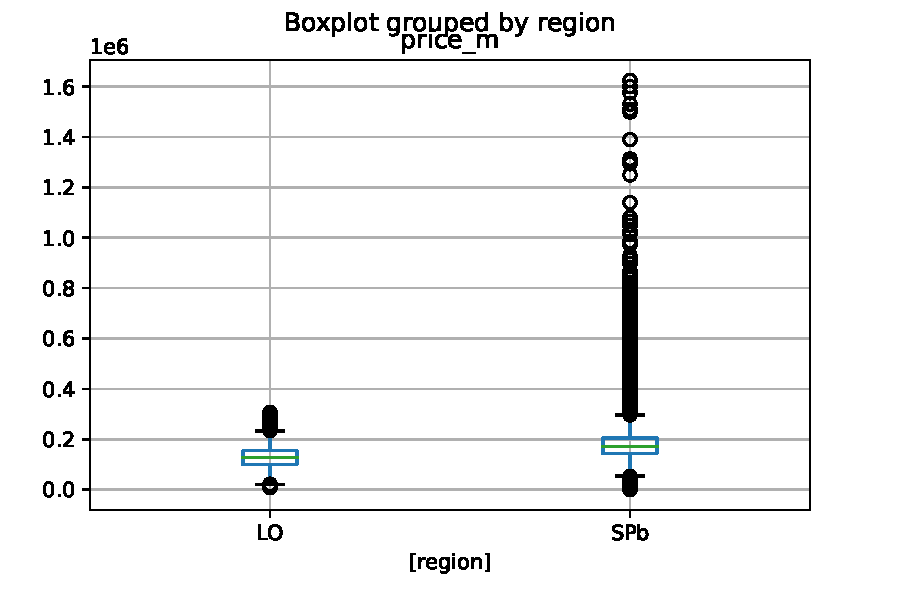
\includegraphics[width=0.95\textwidth]{spb-lo-boxplot-py.pdf}
	\caption{The boxplot diagram for the unit prices of apartment offers in the St. Petersburg agglomeration in the context of regional affiliation.}
	\label{fig:spb-lo-boxplot-py}
\end{figure}

This circumstance allows us to make a subjective judgment that the null hypothesis should be rejected. However, graphical methods of analysis are only suitable for quick primary interpretation, as well as for presentation purposes. Performing the U-test itself will be necessary to form an objective evidentiary judgment.

The normality tests for both dataframes (\textit{dfs}, \textit{dfl}) should be performed to test the applicability of the U-test. There are many criteria for testing the hypothesis that the sample distribution is normal. Three tests were performed in this case:
\begin{itemize}
	\item Shapiro--~Francia test~\cite{Shapiro-Wilk-test};
	\item D'Agostino's K-squared test~\cite{Agostino-test};
	\item Anderson-Darling test~\cite{Anderson-Darling-test}.
\end{itemize}
The Shapiro--~Francia test evaluates a sample of data and calculates how likely it is that it was drawn from a general population that has a normal distribution. This test is considered one of the most powerful normality tests~\cite{Kobzarq-prikl-mathstat}. At the same time, there are some premises indicating that it works well for samples of average size not exceeding five thousand observations (the minimum number is five).

The D'Agostino's K-squared test is based on the analysis of \href{https://en.wikipedia.org/wiki/Skewness}{skewness}~\cite{Wiki:skewness} and ~\href{https://en.wikipedia.org/wiki/Kurtosis}{kurtosis}~\cite{Wiki:kurtosis} indices representing the realizations of the third and fourth \href{https://en.wikipedia.org/wiki/Central_moment}{central moments}~\cite{Wiki:central-moment}, respectively. This test is also considered one of the most powerful and has no limit on the maximum number of observations.

The Anderson-Darling test is a modified version of the \href{https://en.wikipedia.org/wiki/Kolmogorov_Smirnov_test}{Kolmogorov-Smirnov test of goodness-of-fit}~\cite{Wiki:Kolmogorow-Smirnow-test}. It is used to test the hypothesis that the empirical distribution conforms to one of the known theoretical distributions. Its result is not the p-value, but the criterion statistics, unlike the previous two tests.  This requires a more complex interpretation of the result. However, it is already automated in Python.

Let us formulate the null hypotheses:
\begin{itemize}
	\item H0(SPb): the distribution of the values of unit prices of apartment offers in St.~Petersburg does not differ from the normal distribution;
	\item H0(LO): the distribution of the values of apartment supply prices in the territories of the Leningrad Region that are part of the St.~Petersburg agglomeration does not differ from the normal distribution.
\end{itemize} 
Thus, a total of 6 tests will be performed. Their results will be summarized in Table~\ref{tab:normality-tests-values}. All three tests allowed \emph{H0(SPb)} to be rejected for St.~Petersburg data. Two of the three tests also allowed \emph{H0(LO)} to be rejected. We can conclude that the distribution of the subsample containing data about St. Petersburg is unambiguously different from normal, based on the results of the tests. We can also conclude that the distribution of the subsample containing data about the Leningrad region differs from normal with high probability, based on the results of the tests. The use of parametric tests is therefore inappropriate. As a consequence, the U-test discussed above should be used.
%
\begin{lstlisting}[float=htp, caption = Performing the Shapiro-Wilk test for St.~Petersburg data, firstnumber=1, label= lst:shapiro-wilk-test-spb]
stat, p = shapiro(dfs['price_m'])
print('Statistics=%.3f, p=%.3f' % (stat, p))
# interpret
if p <= alpha:
print('Sample does not look Gaussian (reject H0)')
else:
print('Sample looks Gaussian (fail to reject H0)')
\end{lstlisting}
%
\begin{lstlisting}[float=htp, caption = Performing the Shapiro-Wilk test for Leningrad Region data, firstnumber=1, label= lst:shapiro-wilk-test-lo]
stat, p = shapiro(dfl['price_m'])
print('Statistics=%.3f, p=%.3f' % (stat, p))
# interpret
if p <= alpha:
print('Sample does not look Gaussian (reject H0)')
else:
print('Sample looks Gaussian (fail to reject H0)')
\end{lstlisting}  
%
\begin{lstlisting}[float=htp, caption = Performing the D'Agostino's K-squared test for St.~Petersburg data, firstnumber=1, label= lst:K^2-D'Agostino-test-spb]
stat, p = normaltest(dfs['price_m'])
print('Statistics=%.3f, p=%.3f' % (stat, p))
# interpret
if p <= alpha:
print('Sample does not look Gaussian (reject H0)')
else:
print('Sample looks Gaussian (fail to reject H0)')
\end{lstlisting}
%
\begin{lstlisting}[float=htp, caption = Performing the D'Agostino's K-squared test for Leningrad Region data, firstnumber=1, label= lst:K^2-D'Agostino-test-lo]
stat, p = normaltest(dfl['price_m'])
print('Statistics=%.3f, p=%.3f' % (stat, p))
# interpret
if p <= alpha:
print('Sample does not look Gaussian (reject H0)')
else:
print('Sample looks Gaussian (fail to reject H0)')
\end{lstlisting}  
%
\begin{lstlisting}[float=htp, caption = Performing the Anderson-Darling test for St.~Petersburg data, firstnumber=1, label= lst:Anderon-Darling-test-spb]
result = anderson(dfs['price_m'])
print('Statistic: %.3f' % result.statistic)
p = 0
for i in range(len(result.critical_values)):
sl, cv = result.significance_level[i], result.critical_values[i]
if result.statistic < result.critical_values[i]:
print('%.3f: %.3f, data looks normal (fail to reject H0)' % (sl, cv))
else:
print('%.3f: %.3f, data does not look normal (reject H0)' % (sl, cv))
\end{lstlisting}
%
\begin{lstlisting}[float=htp, caption = Performing the Anderson-Darling test for Leningrad Region data, firstnumber=1, label= lst:Anderon-Darling-test-lo]
result = anderson(dfl['price_m'])
print('Statistic: %.3f' % result.statistic)
p = 0
for i in range(len(result.critical_values)):
sl, cv = result.significance_level[i], result.critical_values[i]
if result.statistic < result.critical_values[i]:
print('%.3f: %.3f, data looks normal (fail to reject H0)' % (sl, cv))
else:
print('%.3f: %.3f, data does not look normal (reject H0)' % (sl, cv))
\end{lstlisting}  
%
\begin{table}[htp]
	\caption{The results of the tests of checking the data on the St. Petersburg agglomeration for normality at $\alpha=0.05$.}\label{tab:normality-tests-values}
	\centering
	\begin{tabular}{lll}
		\hline
		The test&St.~Petersburg&Leningrad Region\\
		\hline
		Shapiro-Wilk:&\ref{lst:shapiro-wilk-test-spb}&\ref{lst:shapiro-wilk-test-lo}\\
		criterion statistic~(W)&0.689&0.991\\
		p-value&0.000&0.000\\
		H0&rejected&rejected\\
		\hline
		$K^{2}$ D'Agostino's K-squared test:&\ref{lst:K^2-D'Agostino-test-spb}&\ref{lst:K^2-D'Agostino-test-lo}\\
		criterion statistic~($K^{2}$)&28166.251&4.067\\
	    p-value&0.000&0.131\\
		HO&rejected&can't be rejected\\
		\hline
		Anderson-Darling:&\ref{lst:Anderon-Darling-test-spb}&\ref{lst:Anderon-Darling-test-lo}\\
		criterion statistic~($A^{2}$)&1688.671&15.795\\
		H0:&rejected&rejected\\
		\hline
		Bottom line.:&&\\
		H0&rejected&rejected\\
		\hline
	\end{tabular}
\end{table}
%
Now all that remains is the U-test itself. We use script~\ref{lst:u-test-spba} for this. Its results are presented in Table~\ref{tab:u-test-py-result}. The p-value is less than the specified level of significance. Therefore, we can make the practical conclusion that the difference in the unit value of objects located in the urban and suburban parts of the agglomeration is significant and requires appropriate accounting. Other interpretations of the result can be obtained from the \textit{The alternative hypothesis~(H1)} column of Table\ref{tab:nul-alt-hypothesis-SPba}.
%
\begin{lstlisting}[float=htp, caption = Wilcoxon--~Mann--~Whitney test for the data of unit prices of apartment offers in the agglomeration of St.~Petersburg, firstnumber=1, label= lst:u-test-spba]
stat, p = mannwhitneyu(dfs['price_m'], dfl['price_m'])
print('stat=%.3f, p=%.3f' % (stat, p))
if p <= 0.05:
print('Probably different distributions')
else:
print('Probably the same distribution')
\end{lstlisting}  
%
\begin{table}[htp]
	\caption{The results of the U-test for the St.~Petersburg agglomeration data at $\alpha=0.05$.}\label{tab:u-test-py-result}
	\centering
	\begin{tabular}{ll}
		\hline
		The indicator&Value\\
		\hline
		Criterion statistic&142555441.000\\
		\hline
		p-value&0.000\\
		\hline
		The null hypothesis (see Table~\ref{tab:nul-alt-hypothesis-SPba})&rejected\\
		\hline
		AUC&0.806\\
		\hline
		RBC&0.611\\
		\hline
	\end{tabular}
\end{table}
%
\subsection{ROC analysis, AUC calculation}
The theoretical issues of the relationship between the U-test and the concept of AUC were discussed earlier in~\ref{U-AUC}. A detailed discussion of the practical issues of calculating AUC for real data is given in ~\ref{AUC-almaty}. This subsection will show the code for calculating the AUC and RBC in Python. The code is given in script~\ref{lst:AUC&RBC-spba}. The values obtained along with the other results are shown in Table~\ref{tab:u-test-py-result}.
%
\begin{lstlisting}[float=htp, caption = Calculation of AUC and RBC for St.~Petersburg agglomeration data, firstnumber=1, label= lst:AUC&RBC-spba]
# calculate AUC&RBC
n1n2 = len(dfs.index) * len(dfl.index)
auc = stat/n1n2
rbc = auc-(1-auc)
\end{lstlisting}  
%
\section{R implementation}\label{U-test-R}
%
\lstset{language=R,
	basicstyle=\ttfamily,
	keywordstyle=\color{Blue}\ttfamily,
	stringstyle=\color{Red}\ttfamily,
	commentstyle=\color{Emerald}\ttfamily,
	morecomment=[l][\color{Magenta}]{\#},
	breaklines=true,
	breakindent=0pt,
	breakatwhitespace,
	columns=fullflexible,
	showstringspaces=false
}
%
The R programming language is not as widespread as Python. Although it is quite popular in developed countries. Its area of application is quite niche in Northern Eurasia. It is most often used in scientific activities, especially in biology and chemistry. Knowing this language is more of a bonus than a basic skill for a machine learning specialist. Nevertheless, it should be noted the advantages of R, which include:
\begin{itemize}
	\item a large set of libraries and functions, far superior to the Python toolkit;
	\item very good visualization tools;
	\item handy web development tools such as \textbf{Shiny};
	\item The language is not compiled, but interpreted, which is sometimes more convenient in the case of specific small tasks.
\end{itemize}
The second circumstance is perhaps the main argument in favor of including the R language in the Artificial Intelligence series of publications for appraisers. Python, as a general-purpose language, was originally designed to create compiled executable applications. R is designed for step-by-step data analysis and presentation of all intermediate results.

The choice of the main programming language used by the appraiser depends on the specific task. The use of Python is preferable in the case of developing large complex solutions. It makes sense to pay attention to R in situations where the goal is to solve a specific problem, especially those requiring a serious visualization of the result. In any case, both of these languages have a sufficient set of tools to address the full range of data analysis tasks that arise in the value estimation process.

When writing the R code, its version 4.2.1 (2022-06-23) "Funny-Looking Kid" was used, as well as the IDE RStudio (2022.02.3+492 "Prairie Trillium" Release, 2022-05-20 for Ubuntu Bionic).

Consider another practical problem about the housing market in Almaty. The dataset was provided by Professor G.\,Shoulenbaeva of Narkhoz University. The data file is available \href{https://github.com/Kirill-Murashev/AI_for_valuers_book/blob/main/Parts-Chapters/Mann-Whitney-Wilcoxon/almaty-apts-2019-1.csv}{here}\cite{ds:almaty-apts-2019-1}. The dataset under consideration contains 2355 observations and 12 variables. One of the variables contains information about whether the apartment is offered for sale with or without furniture and appliances. There are three possible values of the variable:
\begin{itemize}
	\item the apartment is sold without furniture and appliances;
	\item the apartment is sold with partial furniture and appliances.;
	\item the apartment is sold with full furniture and appliances. 
\end{itemize}
%
Let's formulate the problem: it is necessary to establish whether or not the equipping of the apartment with movables has any effect on its value. First, the theory of valuation states that in estimating the value of the property the value of only the inseparable improvements of the object should be taken into account. Whereas the value of elements that are movables should be excluded from the value of the object itself. However, in practice, it is often impossible to accurately determine whether an element belongs to the separable or inseparable improvements. It is even more difficult to determine whether analogues have separable improvements. Mathematical analysis of market data will answer the question of whether the problem exists in general. It is possible that the influence of the factor of the presence of improvements having the characteristics of separable, is too insignificant.  Therefore, in any case, it cannot be correctly taken into account in the valuation.  Secondly, the solution of this problem will provide new knowledge about the specific real estate market. For further analysis, we will assume that there are only two options:
\begin{itemize}
	\item sale without potentially separable improvements and chattels;
	\item sale along with potentially separable improvements and chattels.
\end{itemize}
The decision to combine the two categories into one was motivated by three reasons. First, the U-test has certain mathematical limitations and is designed to compare only two samples. There is a non-parametric \href{https://en.wikipedia.org/wiki/Kruskal–Wallis_one-way_analysis_of_variance}{ Kruskal--~Wallis test also known as a one-way ANOVA of ranks} to analyze more than two samples~\cite{Wiki:Kruskal-Wallis}. Second, it is important to understand whether the fact that there are any separable improvements as such has an impact on the value in terms of the theoretical problem outlined above. Third, the division of objects into partially and fully equipped may have been somewhat subjective. Variants of the null and alternative hypotheses are shown in Table~\ref{tab:nul-alt-hypothesis-almaty}.
\begin{table}[htp]
	\caption{The null and alternative hypotheses in the analysis of data from the city of Almaty.} \label{tab:nul-alt-hypothesis-almaty}
	\centering
	\begin{tabularx}{\textwidth}{p{0.15\linewidth} p{0.4\linewidth} p{0.4\linewidth}} 
		\hline
		Type of hypothesis&The null hypothesis~(H0)&The alternative hypothesis~(H1)\\
		\hline
		Scientific&The distributions of the unit values of apartments offered for sale together with separable improvements and chattels and apartments sold without them are the same. There is no shift between the two. The statistical estimates made for a set of objects sold with separable improvements and chattels are unbiased for objects sold without them (the opposite is also true).&The distributions of the unit values of apartments offered for sale together with separable improvements and chattels and apartments offered for sale without them are not equal. There is a shift between the two. The statistical estimate made for a set of properties offered for sale with separable improvements and chattels will be biased for properties offered for sale without them (the opposite is also true).\\
		\hline
		Practical&The median of the unit value of the apartments offered for sale together with the separable improvements and chattels is equal to the median of the unit value of the apartments offered for sale without them.&The median of the unit value of the apartments offered for sale together with the separable improvements and chattels is not equal to the median of the unit value of the apartments offered for sale without them.\\
		\hline
		Set forth in terms of valuation&The presence or absence of separable improvements and chattels in the apartment being sold is not a significant difference and does not require any special consideration. Thus, this attribute is not a pricing factor.&The presence or absence of separable improvements and chattels in the apartment to be sold is a significant difference and requires special accounting. Thus, this attribute is a pricing factor.\\
		\hline
	\end{tabularx}
\end{table}
%
Before you start, you should enable the necessary libraries, set some constants and the path to the working directory, for example as shown in script~\ref{lst:import-libraries-set-constants-set-catalog-R}.
%
\begin{lstlisting}[float=htp, caption = Enables libraries and specifies the values of constants and the path to the working directory, firstnumber=1, label= lst:import-libraries-set-constants-set-catalog-R]
# activate libraries
library(tidyverse)
library(moments)
library(ggplot2)
library(gamlss)
library(normtest)
library(nortest)

# set constants
options('scipen'=2, 'digits'=3)
set.seed(19190709)

# set work catalog
setwd('~/.../Wilcoxon-Mann-Whitney/')
\end{lstlisting}  
%

Next, you need to create a dataframe based on an existing text file with data. It is desirable to leave only the necessary variables \textit{price.m} and \textit{furniture} in order to optimize the use of computing resources. Then convert the dataframe into a more convenient and modern \textbf{tibble} format. See script~\ref{lst:create-dataframe-transform-and-convert-R}. After that, it is necessary to calculate the total number of observations, as well as each type depending on the presence of separable improvements and chattels, see script~\ref{lst:calculate-numbers-of-observations-R}). The results of the count are presented in Table~\ref{tab:numbers-of-observations-almaty-R}.
%
\begin{lstlisting}[float=htp, caption = Creating a dataframe and setting it up, firstnumber=1, label= lst:create-dataframe-transform-and-convert-R]
# create data set from file, create subset with needed variables,
# change the type of object to a more convenient and modern one
almatyFlats <- read.csv('almaty-apts-2019-1.csv', header = TRUE, sep = ",", dec = ".")
myvars <- c('price.m', 'furniture')
almatyFlats <- almatyFlats[myvars]
as_tibble(almatyFlats)
\end{lstlisting} 
%
\begin{lstlisting}[float=htp, caption = Counting the number of observations, firstnumber=1, label= lst:calculate-numbers-of-observations-R]
# calculation of the total number of observations,
# as well as depending on the equipment 
n.total <- nrow(almatyFlats)
n.non.equip <- NROW(almatyFlats$furniture[ which(almatyFlats$furniture == 0)])
n.equip <- NROW(almatyFlats$furniture[ which(almatyFlats$furniture > 0)]))
\end{lstlisting}
%
For the purposes of primary visualization of the data, we plot histograms for observations of all types. This time the number of columns will be determined by the formula developed in 1991 by P.\,W.~Nowiczkij~\cite{Nowiczkij:oczenka-pogresh}.
\begin{equation}\label{eq:k-hist_Nowiczkij}
k = \frac{1}{3}\sqrt[5]{\varepsilon^4 n^2} \equiv \frac{1}{3} \sqrt[5]{\frac{n^2}{\xi^8}}, 
\end{equation}
where $\varepsilon$ --- is the kurtosis coefficient, $\xi$ --- is the counter kurtosis coefficient. First, let's create an appropriate function for convenience  (script~\ref{lst:k-number-Nowiczkij-R}). Then we calculate a rational number of intervals for the entire data set and separately for apartments offered for sale without and with separable improvements and chattels (see script~\ref{lst:k-number-R}). The results of the calculation are shown in Table~\ref{tab:numbers-of-observations-almaty-R}.
%
\begin{lstlisting}[float=htp, caption = Create a function to calculate~k using Nowiczkij's formula, firstnumber=1, label= lst:k-number-Nowiczkij-R]
# create function for second Nowiczkij formula
kHistNowiczkij2 <- function(x, na.omit = FALSE){ # create function, ignore missed values
n   <- NROW(x)                                 # calculate n
kurt = kurtosis(x)                             # calculate kurtosis
kn2 = (((kurt^4)*(n^2))^(1/5))*(1/3)           # calculate k
return(kn2)                                    # return k  
}                                              # end of function
\end{lstlisting} 
%
\begin{lstlisting}[float=htp, caption = Calculation of~k for observations of different types by Nowiczkij's formula., firstnumber=1, label= lst:k-number-R]
# calculation numbers of k for different types of observations
k.all.data <- kHistNowiczkij2(almatyFlats$price.m)
k.non.equip <- kHistNowiczkij2(almatyFlats$price.m[ which(almatyFlats$furniture == 0)])
k.equip <-kHistNowiczkij2(almatyFlats$price.m[ which(almatyFlats$furniture > 0)])                                       
\end{lstlisting}
%
\begin{table}[htp]
	\caption{Information about the number of observations of different types in the market of Almaty.}\label{tab:numbers-of-observations-almaty-R}
	\centering
	\begin{tabular}{lll}
		\hline
		Type of observation.&Number of&Rational number of intervals~(k).\\
		\hline
		All observations.&2355&36\\
		\hline
		Observations without separable improvements and chattels&605&22\\
		\hline
		Observations with separable improvements and chattels&1750&31\\
		\hline
	\end{tabular}
\end{table}
%
Let's plot histogram for all observations (Diagram~\ref{fig:almaty-hist-all-r}), those that are equipped (Diagram~\ref{fig:almaty-hist-equiped-r}) and those that are sold without any separable improvements (Diagram~\ref{fig:almaty-hist-nequiped-r}). The diagrams show that the distributions have heavy right tails. This indirectly indicates that the distribution in all three cases differs from the normal one. Quantitative tests of normality will be performed later to form an informed judgment. The code for histograms is given in script~\ref{lst:plot-hist-R}. The basic descriptive statistics for each of the three types of observations are given in Table~\ref{tab:summaries-almaty-R}. They were calculated using script~~\ref{lst:summaries-R}. The boxplot diagram was built using script~\ref{lst:boxplot-R}. It is shown in Diagram~\ref{fig:almaty-boxplot-r}. As you can see, the median price of properties offered for sale with separable improvements and chattels is higher than the median price of properties offered for sale without them.
%
\begin{lstlisting}[float=htp, caption = Plotting histograms for observations of different types, firstnumber=1, label= lst:plot-hist-R]
# plot the histogram, combined with the density curve of the theoretical
# normal distribution for all observations
histDist(almatyFlats$price.m,
density = TRUE,
nbins = kHistNowiczkij2(almatyFlats$price.m),
xlab = 'price per meter, kaz tenge',
ylab = 'probability',
main = 'Price per meter histogram, all observations')

# plot the histogram, combined with the density curve of the theoretical
# normal distribution for observations without equipment
histDist(almatyFlats$price.m[ which(almatyFlats$furniture == 0)],
density = TRUE,
nbins = kHistNowiczkij2(almatyFlats$price.m[ which(almatyFlats$furniture == 0)]),
xlab = 'price per meter, kaz tenge',
ylab = 'probability',
main = 'Price per meter histogram, observations witout equipment')

# plot the histogram, combined with the density curve of the theoretical
# normal distribution for observations with equipment
histDist(almatyFlats$price.m[ which(almatyFlats$furniture > 0)],
density = TRUE,
nbins = kHistNowiczkij2(almatyFlats$price.m[ which(almatyFlats$furniture > 0)]),
xlab = 'price per meter, kaz tenge',
ylab = 'probability',
main = 'Price per meter histogram, observations witout equipment')
\end{lstlisting}
%
\begin{lstlisting}[float=htp, caption = Calculation of basic descriptive statistics for observations of different types, firstnumber=1, label= lst:summaries-R]
# summaries
summary(almatyFlats$price.m)
summary(almatyFlats$price.m[ which(almatyFlats$furniture == 0)])
summary(almatyFlats$price.m[ which(almatyFlats$furniture > 0)])
\end{lstlisting}
%
\begin{figure}[htp]
	\centering
	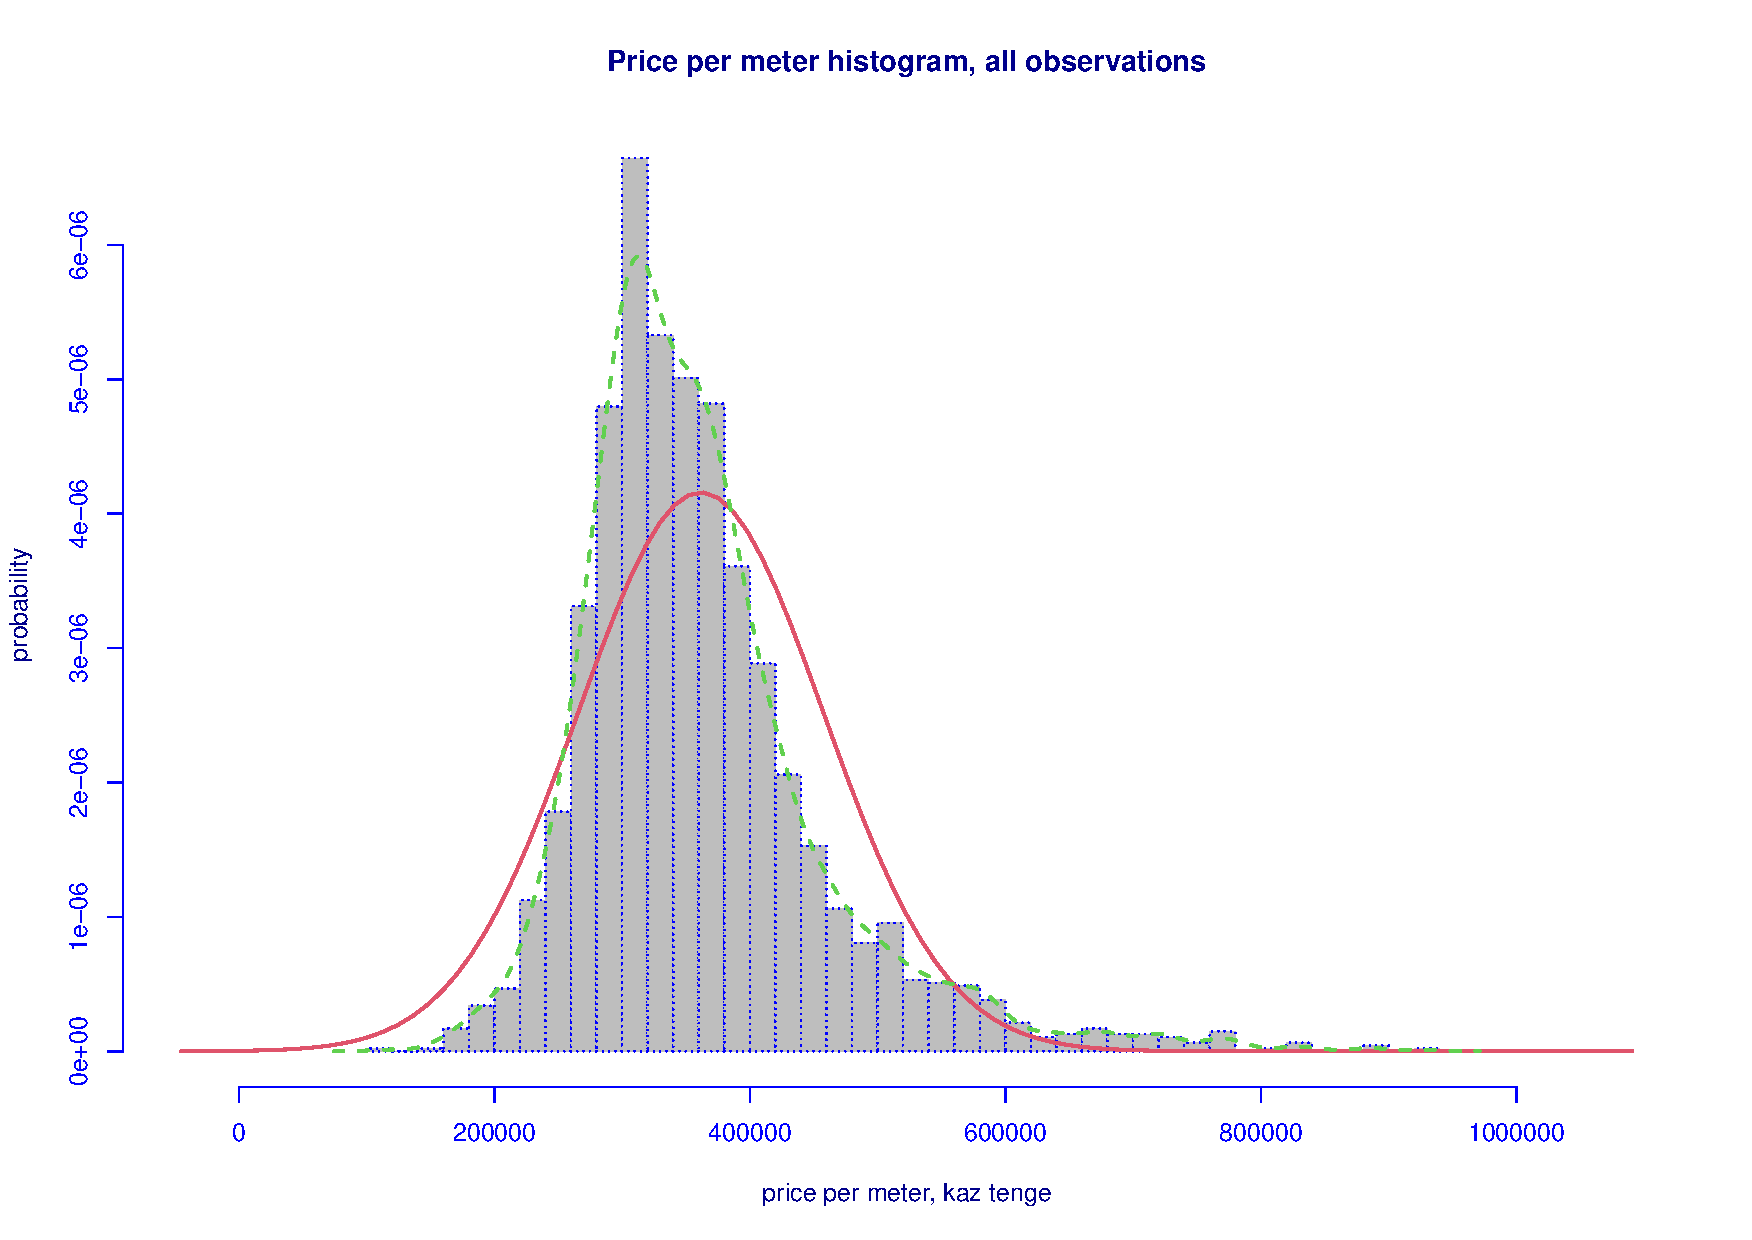
\includegraphics[width=0.95\textwidth]{almaty-hist-all.pdf}
	\caption{Histogram of bid prices for all objects. Combined with the density function curve of the empirical distribution, as well as the density function curve of the theoretical normal distribution.}
	\label{fig:almaty-hist-all-r}
\end{figure}
%
%
\begin{figure}[htp]
	\centering
	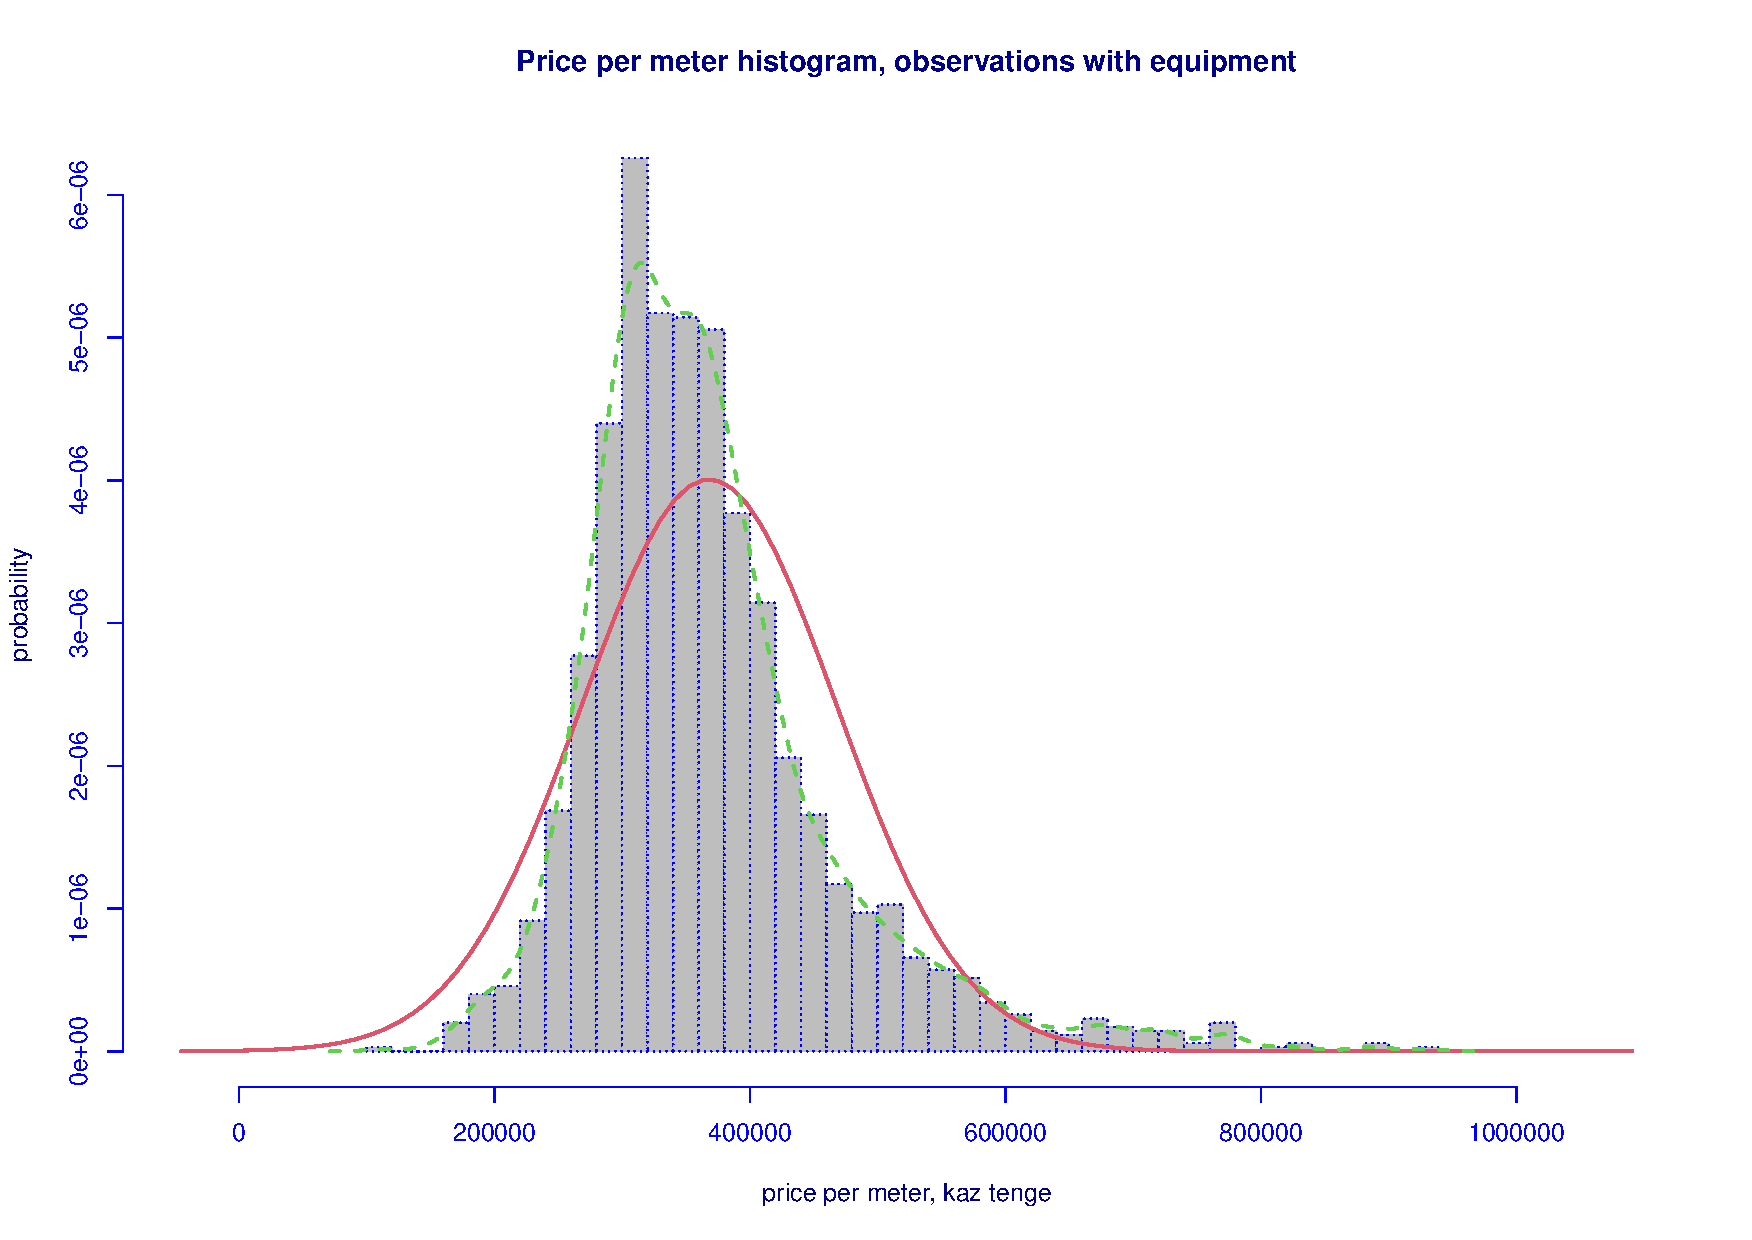
\includegraphics[width=0.95\textwidth]{almaty-hist-equiped.pdf}
	\caption{Histogram of bid prices for properties offered for sale together with separable improvements and chattels. Combined with the density function curve of the empirical distribution, as well as the density function curve of the theoretical normal distribution.}
	\label{fig:almaty-hist-equiped-r}
\end{figure}
%
%
\begin{figure}[htp]
	\centering
	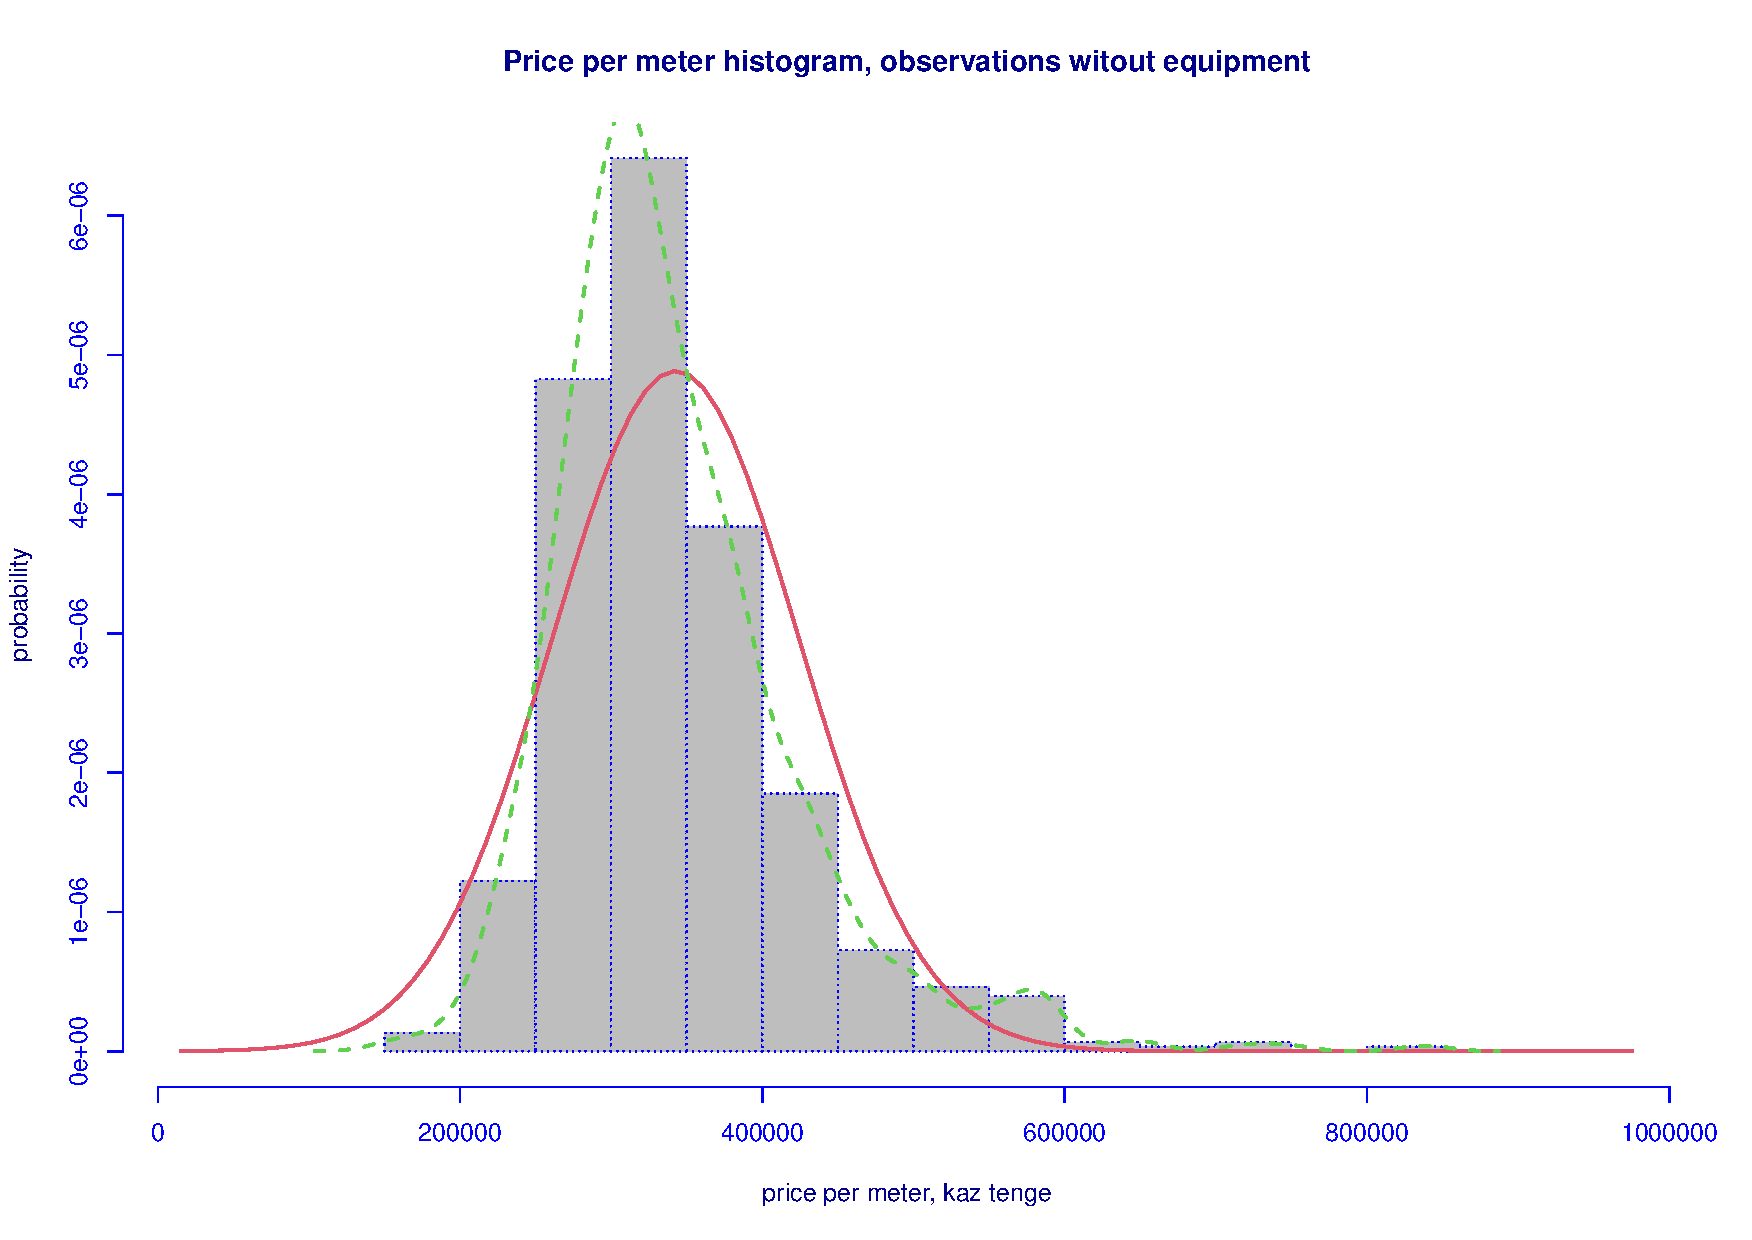
\includegraphics[width=0.95\textwidth]{almaty-hist-nequiped.pdf}
	\caption{Histogram of bid prices for properties offered for sale without separable improvements and chattels. Combined with the density function curve of the empirical distribution, as well as the density function curve of the theoretical normal distribution.}
	\label{fig:almaty-hist-nequiped-r}
\end{figure}
%
\begin{table}[htp]
	\caption{Basic descriptive statistics of observations of different types in the market of Almaty. The unit of measure is the Kazakhstani tenge.}\label{tab:summaries-almaty-R}
	\centering
	\begin{tabular}{lllllllll}
		\hline
		Type of observation.&Min&1Q&Median&Mean&3Q&Max\\
		\hline
		All observations&117000&300000&344432&361554&400000&928571\\
		\hline
		Observations without separable improvements and chattels&152542&291803&325581&342581&378788&838462\\
		\hline
		Observations with separable improvements and chattels&117000&305446&350331&368113&406183&928571\\
		\hline
	\end{tabular}
\end{table}
%
\begin{figure}[htp]
	\centering
	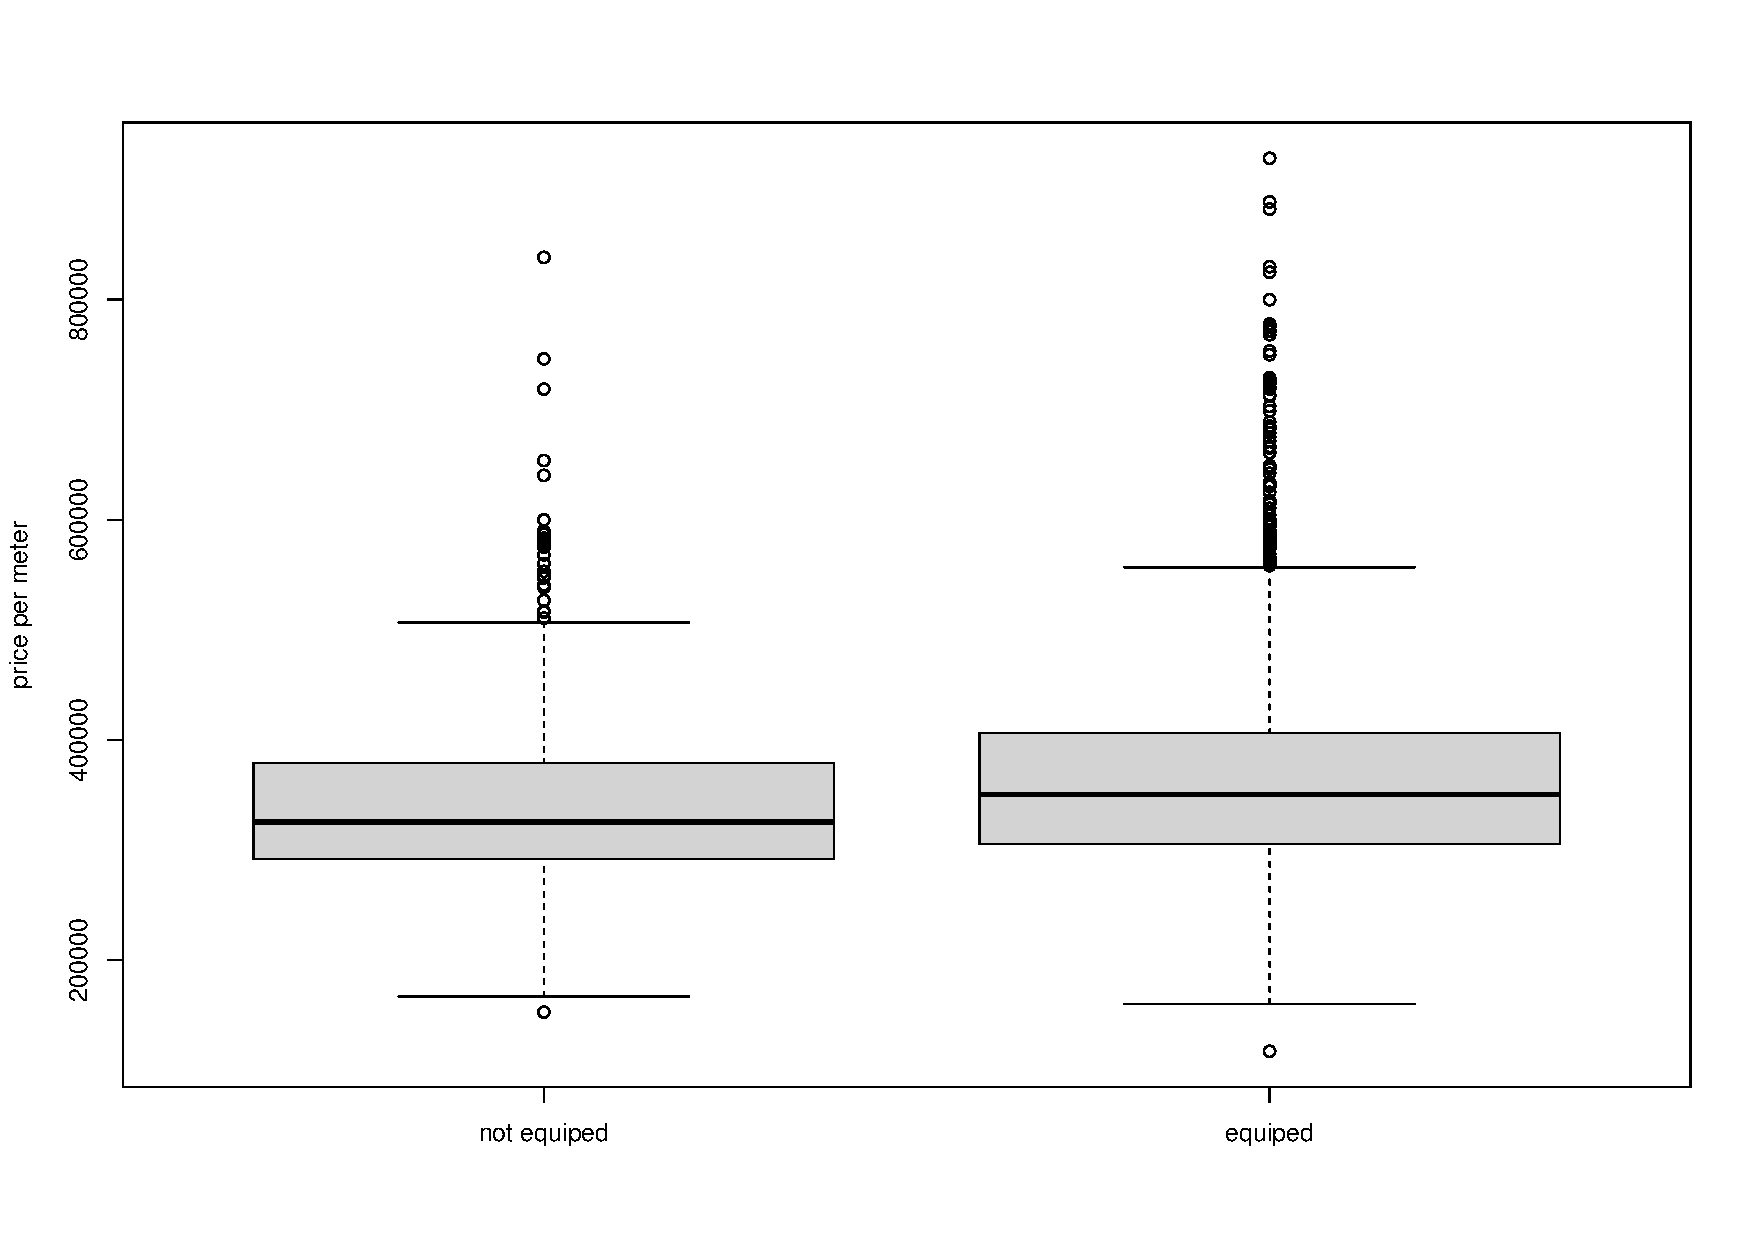
\includegraphics[width=0.95\textwidth]{almaty-boxplot.pdf}
	\caption{Boxplot for the market of Almaty.}
	\label{fig:almaty-boxplot-r}
\end{figure}
%
\begin{lstlisting}[float=htp, caption = Plotting boxplot diagram for the market of Almaty, firstnumber=1, label= lst:boxplot-R]
# plot boxplots
nequiped <- subset(almatyFlats, furniture == 0)
equiped <- subset(almatyFlats, furniture > 0)
boxplot(nequiped$price.m, equiped$price.m,
ylab = 'price per meter',
names =c('not equiped', 'equiped'))
rm(nequiped)
rm(equiped)
\end{lstlisting}
%

The next stage of the analysis is to check the normality of the distribution of unit bid prices. The R~language has a very wide range of tools as mentioned above. There are many libraries offering a total of several dozen tests. The following tests were applied in this paper.
\begin{itemize}
	\item the Shapiro--~Wilk test~\cite{Shapiro-Wilk-test};
	\item the Shapiro--~Francia test~\cite{Shapiro-Francia-test};
	\item the Anderson--~Darling test~\cite{Anderson-Darling-test};
	\item the adjusted Jarque--~Bera test~\cite{Jarque-Bera-test};
	\item the Lilliefors' test~\cite{Liliefors-normality-test}.
\end{itemize}
The code for running tests for objects without and with separable improvements is given in scripts~\ref{lst:normality-tests-nequiped-R} and~\ref{lst:normality-tests-equiped-R}, respectively. The test results for the subsamples are summarized in Table~\ref{tab:normality-tests-values-R}. The results of all tests allow us to draw an unambiguous conclusion: the distributions of both subsamples differ from the normal one. This points to the need to use nonparametric criteria.
%
\begin{lstlisting}[float=htp, caption = Performing normality tests for observations without separable improvements and chattels, firstnumber=1, label= lst:normality-tests-nequiped-R]
# normality tests for non equipped observations
# Shapiro-Wilk test for normality
shapiro.test(almatyFlats$price.m[ which(almatyFlats$furniture == 0)])
# Shapiro-Francia test for normality
sf.test(almatyFlats$price.m[ which(almatyFlats$furniture == 0)])
# Anderson-Darling test for normality
ad.test(almatyFlats$price.m[ which(almatyFlats$furniture == 0)])
# Adjusted Jarque-Bera test for normality
ajb.norm.test(almatyFlats$price.m[ which(almatyFlats$furniture == 0)])
# Lilliefors (Kolmogorov-Smirnov) test for normality
lillie.test(almatyFlats$price.m[ which(almatyFlats$furniture == 0)])
\end{lstlisting}
%
\begin{lstlisting}[float=htp, caption = Performing normality tests for observations with separable improvements and chattels, firstnumber=1, label= lst:normality-tests-equiped-R]
# normality tests for non equipped observations
# Shapiro-Wilk test for normality
shapiro.test(almatyFlats$price.m[ which(almatyFlats$furniture > 0)])
# Shapiro-Francia test for normality
sf.test(almatyFlats$price.m[ which(almatyFlats$furniture > 0)])
# Anderson-Darling test for normality
ad.test(almatyFlats$price.m[ which(almatyFlats$furniture > 0)])
# Adjusted Jarque-Bera test for normality
ajb.norm.test(almatyFlats$price.m[ which(almatyFlats$furniture > 0)])
# Lilliefors (Kolmogorov-Smirnov) test for normality
lillie.test(almatyFlats$price.m[ which(almatyFlats$furniture > 0)])
\end{lstlisting}
%

\begin{table}[htp]
	\caption{The results of normality tests for the data on the Almaty market at $\alpha=0.05$.}\label{tab:normality-tests-values-R}
	\centering
	\begin{tabular}{lll}
		\hline
		Test name&Without inseparable improvements&Without inseparable improvements\\
		\hline
		Shapiro--~Wilk&\ref{lst:normality-tests-nequiped-R}&\ref{lst:normality-tests-equiped-R}\\
		criterion statistic~(W)&0.9&0.9\\
		p-value&<2e-16&<2e-16\\
		H0&rejected&rejected\\
		\hline
		Shapiro--~Francia&\ref{lst:normality-tests-nequiped-R}&\ref{lst:normality-tests-equiped-R}\\
		criterion statistic~(W)&0.9&0.9\\
		p-value&<2e-16&<2e-16\\
		H0&rejected&rejected\\
		\hline
		Anderson--~Darling&\ref{lst:normality-tests-nequiped-R}&\ref{lst:normality-tests-equiped-R}\\
		criterion statistic~(A)&13&42\\
		p-value&<2e-16&<2e-16\\
		H0&rejected&rejected\\
		\hline
		Jarque--~Bera (adj.)&\ref{lst:normality-tests-nequiped-R}&\ref{lst:normality-tests-equiped-R}\\
		criterion statistic~(AJB)&757&1720\\
		p-value&<2e-16&<2e-16\\
		H0&rejected&rejected\\
		\hline
		Lilliefiors (K--~S)&\ref{lst:normality-tests-nequiped-R}&\ref{lst:normality-tests-equiped-R}\\
		criterion statistic~(D)&0.1&0.1\\
		p-value&<2e-16&<2e-16\\
		H0&отклоняется&отклоняется\\
		\hline
		The final conclusion&&\\
		H0&rejected&rejected\\
		\hline
	\end{tabular}
\end{table}
%
To perform a U-test, just run the code contained in script~\ref{lst:U-test-R}. The results of the test are shown in Table~\ref{tab:u-test-r-result}. Based on this result, we can conclude that the factor of the presence of inseparable improvements and chattels must be taken into account.
%
\begin{lstlisting}[float=htp, caption = Running a U-test for data from the city of Almaty., firstnumber=1, label= lst:U-test-R]
# perform Mann-Whitney U-test
wilcox.test(almatyFlats$price.m[ which(almatyFlats$furniture == 0)],
almatyFlats$price.m[ which(almatyFlats$furniture > 0)]) 
\end{lstlisting}
%
\begin{table}[htp]
	\caption{Results of the U-test for the Almaty data at$\alpha=0.05$.}\label{tab:u-test-r-result}
	\centering
	\begin{tabular}{ll}
		\hline
		Indicator&Value\\
		\hline
		Criterion statistic&441360\\
		\hline
		p-value&1e-09\\
		\hline
		The null hypothesis (see Table~\ref{tab:nul-alt-hypothesis-almaty})&rejected\\
		\hline
		AUC&0.583\\
		\hline
		RBC&0.166\\
		\hline
	\end{tabular}
\end{table}
%
\subsection{AUC issues}
\subsubsection{AUC calculation}\label{AUC-almaty}
The theoretical issues of the relationship between the U-test and the concept of AUC were discussed earlier in Chapter~\ref{U-AUC}. Note only that the AUC, which is a quantitative estimate of the area under the ROC curve, is a widely used characteristic of the quality of a binary classifier. Surprisingly, the AUC is directly related to the U-statistic. This subsection will calculate the AUC and show the relationship between it and the U-test. Let's add \textit{labels} vector to the existing dataframe. It contains binary labels indicating the presence or absence of inseparable improvements and chattels in a particular observation. See script~\ref{lst:create-labels-vector-R}. Thus, the \textit{price.m} variable is a vector of scores, and the \textit{labels} variable is a vector of labels.
%
\begin{lstlisting}[float=htp, caption = Adding a variable with binary labels. firstnumber=1, label= lst:create-labels-vector-R]
# create vector for labels
almatyFlats$labels <- rep(0, length(almatyFlats$price.m))

# set values by condition
almatyFlats$labels[almatyFlats$furniture > 0] <- 1
\end{lstlisting}
%

Let's create our own function to calculate AUC based on Formula~\ref{eq:AUC}, where $U_{1}$ is the test statistic. And then apply it to the data. Let's write script~\ref{lst:create&apply-owm-WMW-AUC-function-R} to do this. The returned AUC value was \textbf{0.583}. It can be interpreted as follows: \emph{the probability that the unit value of a random observation (object-analogues) offered for sale together with separable improvements and movable property is higher than that of a random observation offered for sale without separable improvements and movable property is equal to 0.583}.
%
\begin{lstlisting}[float=htp, caption = Create your own function to calculate the AUC and apply it to the data of the Almaty market., firstnumber=1, label= lst:create&apply-owm-WMW-AUC-function-R]
# create function to calculate AUC
auc_wmw <- function(labels, scores){
labels <- as.logical(labels)
pos <- scores[labels]
neg <- scores[!labels]
U <- as.numeric(wilcox.test(pos, neg)$statistic)
U/(length(pos) * length(neg))
}

# apply auc_wmw to data
auc_wmw(almatyFlats$labels, almatyFlats$price.m)
\end{lstlisting}
%

Let's also create our own function to calculate the U-statistic according to Formula~\ref{eq:U1} for better understanding of further actions. The values of "positive cases" (observations with inseparable improvements and chattels) will be taken as~$R_{1}$ and~$n_{1}$. Naturally, calculating U-statistic for "negative" cases ($R_{2},\ n_{2}$) is also possible. The U1 and U2 statistics are complementary with respect to each other, because their sum is always equal to~$n_{1} \times n_{2}$. Using the U2 statistic causes the ROC curve to flip. Hense $AUC_{2}=1-AUC_{1}$. The U-test has previously been shown to be related to the Bayesian approach to probability. Therefore, there is no need to determine what is a positive and negative case using any special methods. A priori knowledge that properties offered for sale together with separable improvements and chattels are worth more than properties offered for sale without them is sufficient. The code to create such a function is given in Script~\ref{lst:create&apply-owm-U-stat-function-R}. The returned value of AUC was 0.583. Within our function \texttt{auc\_wmw} we use our own function \texttt{rank}. It works as follows: the observation with the lowest value is assigned a rank of 1 (if there are no ties). Then the ranks are assigned as the value of scores increases. In the case of bundles, such observations are assigned a median value of the entire group.
%
\begin{lstlisting}[float=htp, caption = Creation of own function to calculate U-statistic and its application to Almaty market data, firstnumber=1, label= lst:create&apply-owm-U-stat-function-R]
create function to calculate AUC in different way
auc_wmw2 <- function(labels, scores){
labels <- as.logical(labels)
n1 <- sum(labels)
n2 <- sum(!labels)
R1 <- sum(rank(scores)[labels])
U1 <- R1 - n1 * (n1 + 1)/2
U1/(n1 * n2)
}

# apply auc_wmw2 to data
auc_wmw2(almatyFlats$labels, almatyFlats$price.m)
\end{lstlisting}
%

In what follows, the rationale for the equivalence of the concept of AUC and the value resulting from the application of the formula~\ref{eq:U1} will be given.
%
\subsubsection{Graphical interpretation ot the U-statistic}
Let's plot a diagram, on which horizontal bars will be laid out the ranks of observations. Positive observations are colored green, negative observations are colored red. Code~\ref{lst:vizualize-pos&neg-cases-almaty-R} was used to do this. The result was Diagram~~\ref{fig:pos&neg-ranks-vizualize-r.pdf}.
%
\begin{lstlisting}[float=htp, caption = Visualization of the ranks of positive and negative observations for the Almaty market, firstnumber=1, label= lst:vizualize-pos&neg-cases-almaty-R]
# create function to prepare data for plotting
u_illustration_part1 <- function(labels, scores){
# put cases in order by score
sort_order <- order(scores)
labels <- labels[sort_order]
scores <- scores[sort_order]

# count the cases
n <- length(labels)

# find overall rank for each case by score
ranks <- rank(scores)

# start with an empty plot
plot(c(0, n), c(0, n), type='n', xlim = c(0, 2500),
xlab="rank", ylab="case", asp=1)

# plot bars representing ranks of all cases
mapply(rectangle, x=0, y=(n - 1):0,  # starting from the top 
width=ranks, height=1, 
density=NA, lwd=2, col=c("red", "green")[1 + labels])
# set labels   
legend("topright", legend=c("negative cases (no furniture & equipment)", "positive cases (with furniture & equipment)"), 
text.col=c("red", "green"), bty='o', box.lwd=1, inset=0.1)
}

# apply function to data
u_illustration_part1(labels=almatyFlats$labels, scores=almatyFlats$price.m)
\end{lstlisting}
%
\begin{figure}[htp]
	\centering
	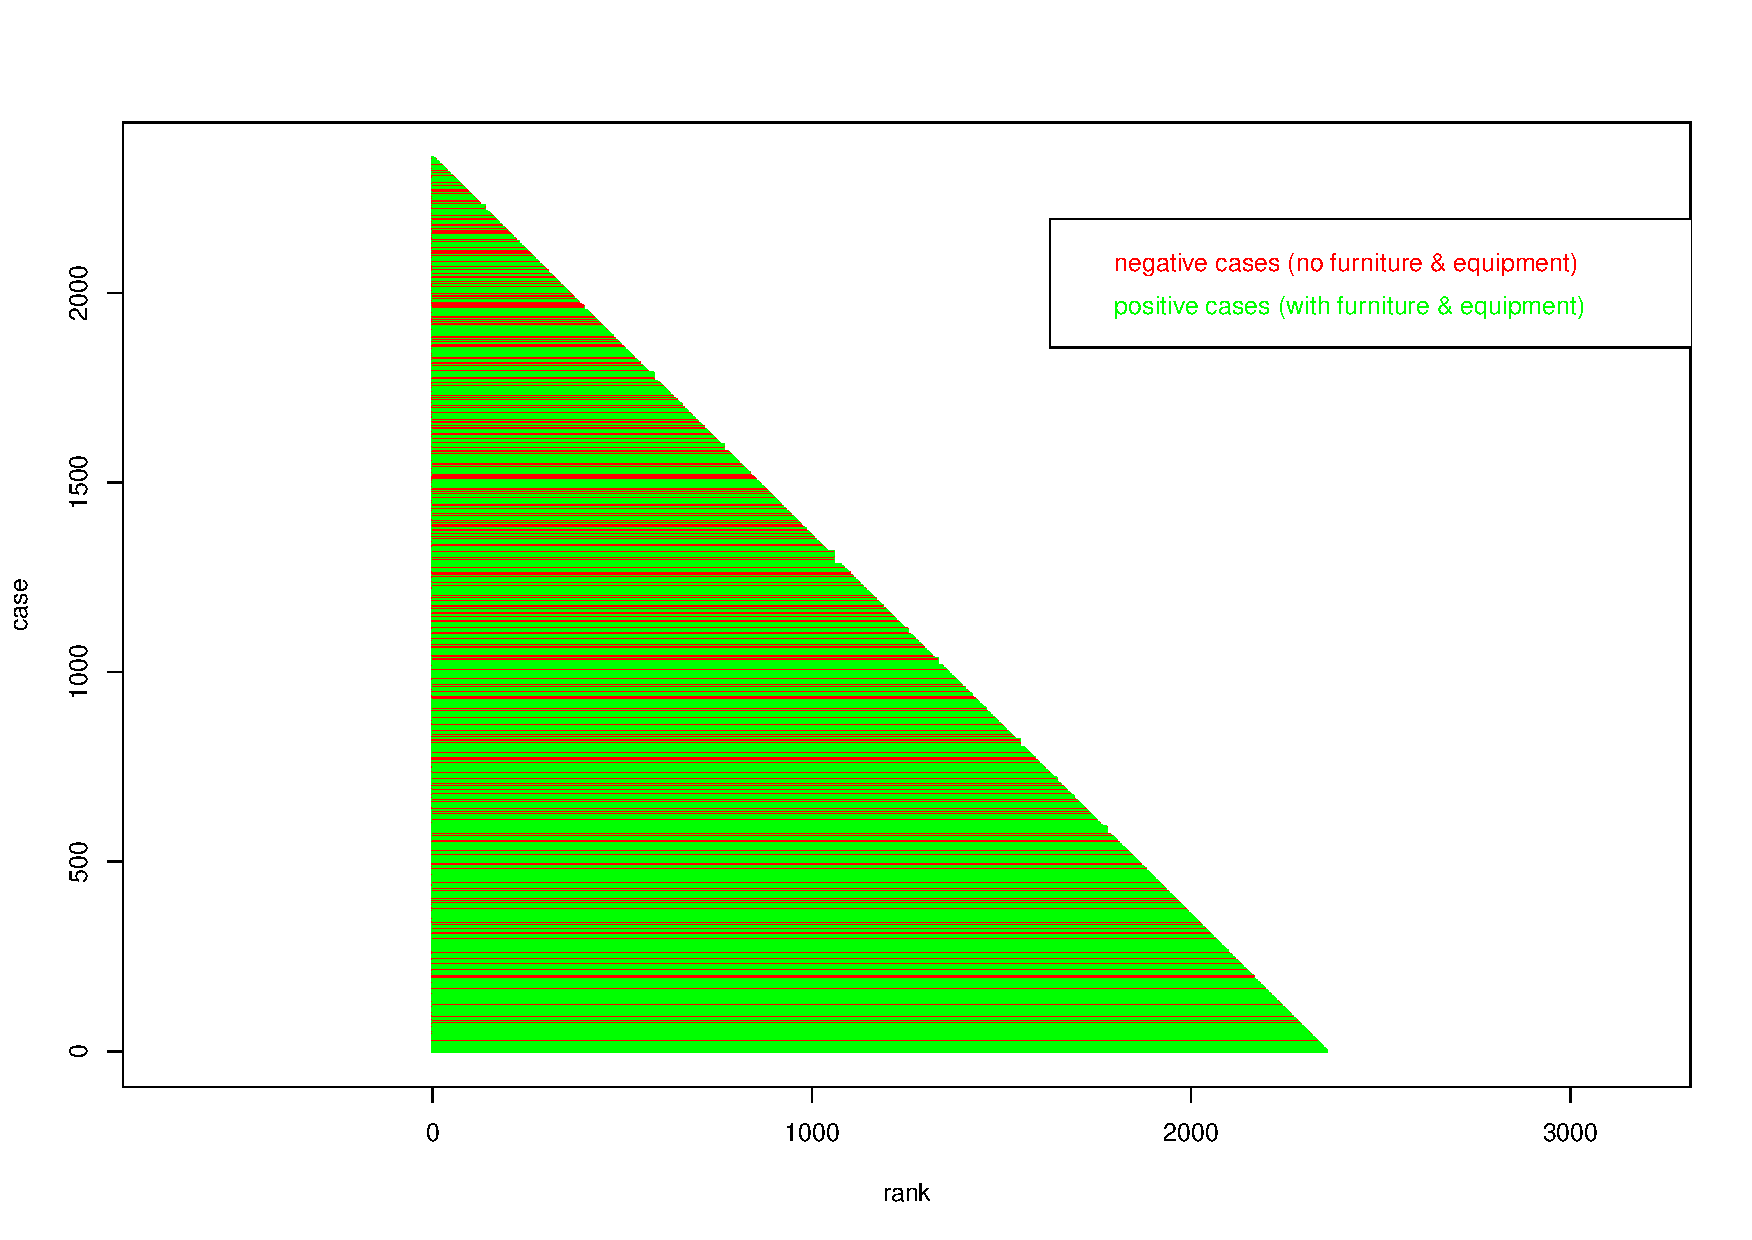
\includegraphics[width=0.95\textwidth]{pos&neg-ranks-vizualize-r.pdf}
	\caption{Visualization of the ranks of positive and negative observations for the Almaty market.}
	\label{fig:pos&neg-ranks-vizualize-r.pdf}
\end{figure}
%

Now consider only the positive cases shown by the green bars. Let's stack them sequentially on top of each other, shifting to the right as negative cases meet. See script~~\ref{lst:vizualize-pos-cases-almaty-R}. In this way we get a sequence of graduated steps. Consider Diagram 5~\ref{fig:pos-ranks-vizualize-r.pdf}. The total area of green bands is equivalent to the value of~$R_{1}$, calculated according to the logic of formula~\ref{eq:common-R}. The red box on the right represents the part we will subtract. Note that the total area of the green bars inside the shaded red square is equal to
\begin{equation}\label{eq:R-1}
S_{green-bars-right-side}=\frac{n_{1}(n_{1}+1)}{2},
\end{equation}
which is the sum of integers from~1 to~$n_{1}$. The rectangle highlighted by the black dotted line on the left side represents the part that we will keep. The green area inside it (the sum of the green bars) represents the value of the $U_{1}$ statistic. In this case, $n_{1}$ is the number of steps on the y-axis, obviously equal to the number of green bars. Less obvious is that $n_{2}$ is the number of steps "to the East" inside the black rectangle. It matches to the number of missed negative observations. This graph is a graphical representation of the formula for calculating of~$U_{1}$. The area of the entire black rectangle grid is~$n_{1} \times n_{2}$. Then $U_{1}$ represents the absolute value of the area under the curve. The~$U_{1}$ should be divided by~$n_{1} \times n_{2}$ to normalize the value. This operation is exactly the same as the academic formula~\ref{eq:AUC} used to calculate the AUC for the U-test. The practice of normalizing values follows from the rules of ROC analysis, which further indicates that the U-test is related to machine learning techniques.

The blue line represents the ROC curve built with the regular \texttt{roc} function from the \textbf{pROC} library. It is scaled by $n_{2}$ on the x-axis~(FPR) and by $n_{1}$ on the y-axis~(TPR). In the case of bars representing unique ranks, it coincides with their left edge. In the case of ties, it divides the bar vertically as a diagonal pointing "to the Northeast".
%
\begin{lstlisting}[float=htp, caption = Visualization of the ranks of positive and negative observations for the Almaty market, firstnumber=1, label= lst:vizualize-pos-cases-almaty-R]
# create function to stack positive cases
u_illustration_part2 <- function(labels, scores){
# sort the cases
sort_order <- order(scores)
labels <- labels[sort_order]
scores <- scores[sort_order]

# count positive and negative cases
n1 <- sum(labels)  # number of positive cases
n2 <- sum(!labels) # number of negative cases

# find the overall ranks for the positive cases
ranks <- rank(scores)
pos_ranks <- ranks[as.logical(labels)]

# how far to slide each bar to make stairsteps on the right hand edge
x_offset <- n2 + (1:n1) - pos_ranks

# start with an empty plot  
plot(c(0, n2 + n1), c(0, n1), type='n', asp=1,
xlab="n2 + n1 divisions", ylab="n1 divisions")

# plot bars for ranks of positive cases
mapply(rectangle, x=x_offset, y=(n1 - 1):0, 
width=pos_ranks, height=1,
density=NA, border="darkgreen", lwd=2, col="green")

# mark the area we remove, and the area we keep
rectangle(n2, 0, n1, n1, density=10, col="red", lwd=1)
rectangle(0, 0, n2, n1, density=0, col="black", lty=2, lwd=3)

# draw a scaled version of the "official" ROC curve on top
roc_obj <- roc(labels, scores)
roc_df <- with(roc_obj, data.frame(FPR=rev(1 - specificities), 
TPR=rev(sensitivities)))
with(roc_df, lines(n2*FPR, n1*TPR, type='l', lwd=4, col="blue"))
}

# apply function to data
u_illustration_part2(labels=almatyFlats$labels, scores=almatyFlats$price.m)
\end{lstlisting}
%
\begin{figure}[htp]
	\centering
	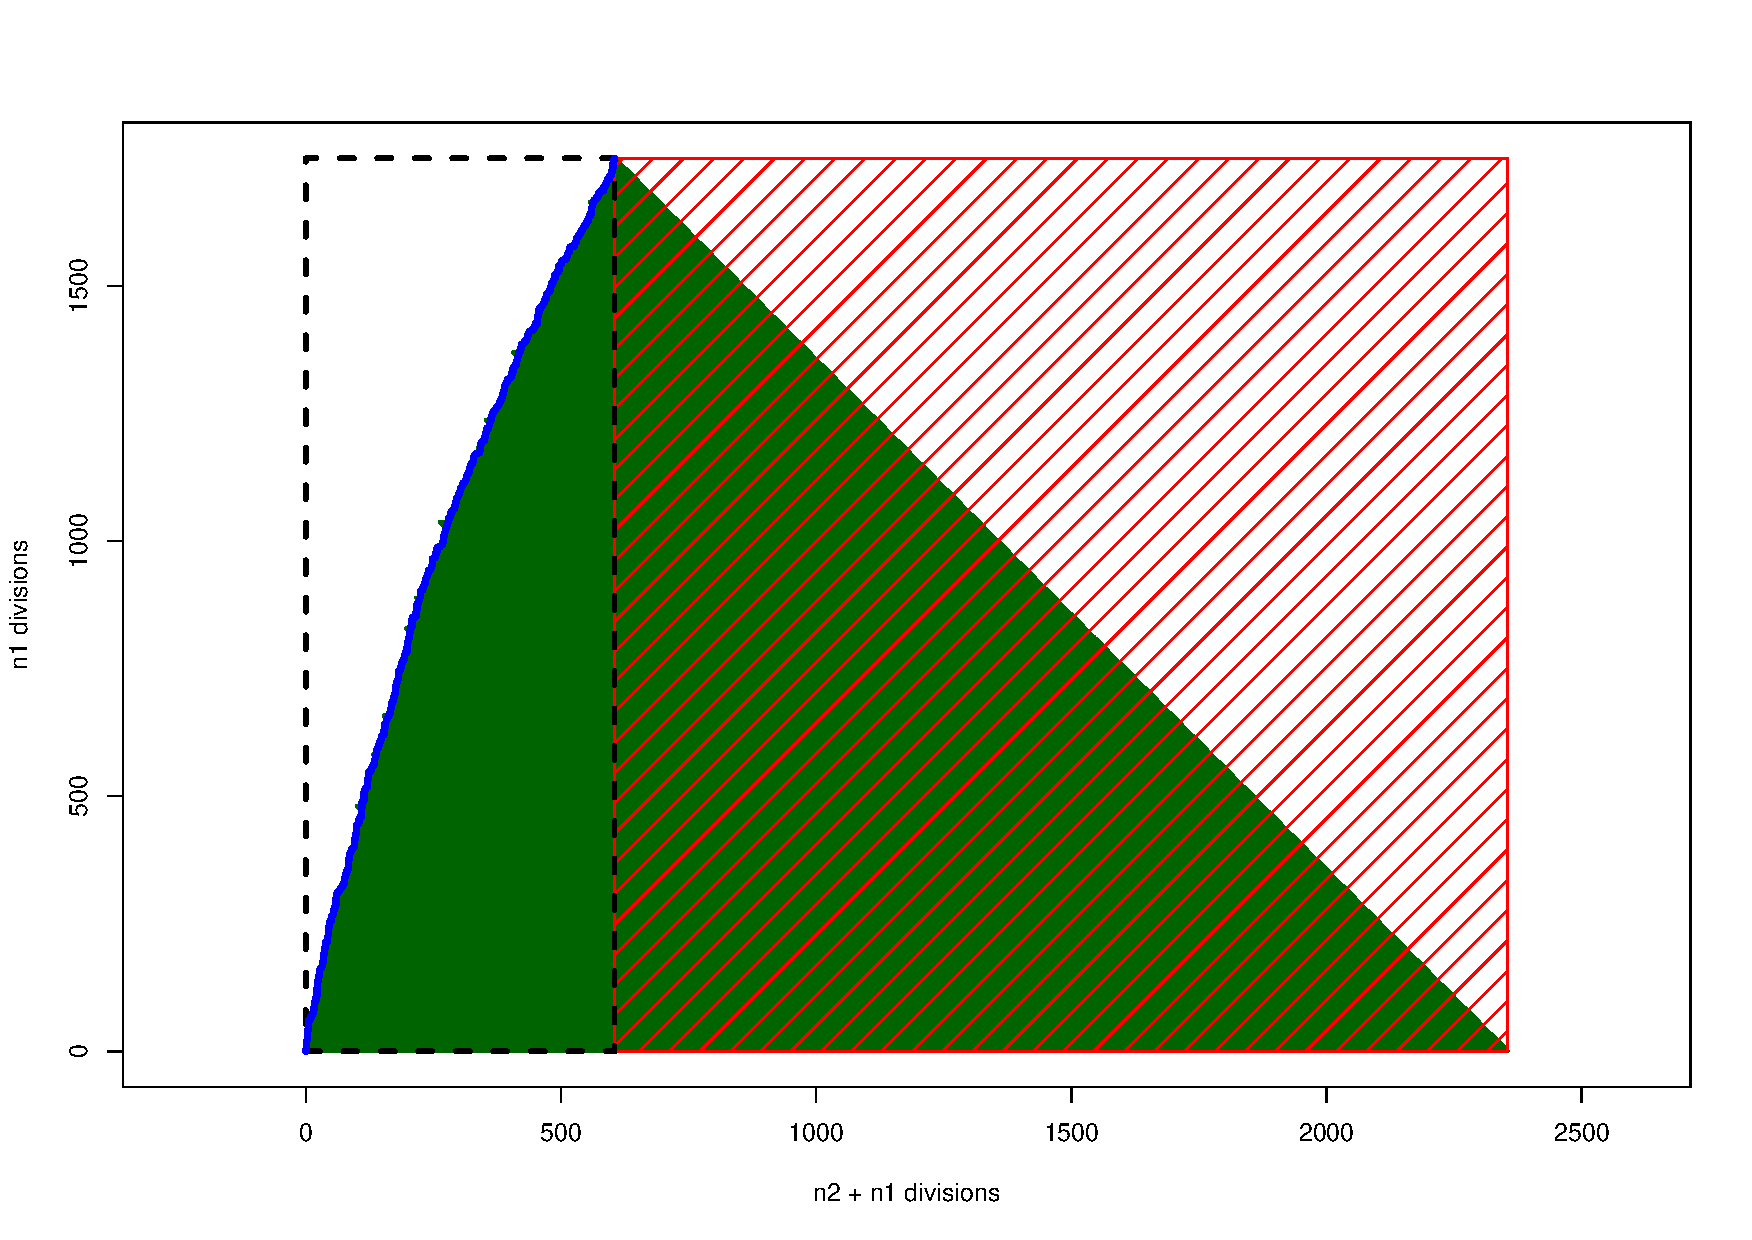
\includegraphics[width=0.95\textwidth]{pos-ranks-vizualize-r.pdf}
	\caption{Visualization of the ranks of positive and negative observations for the Almaty market.}
	\label{fig:pos-ranks-vizualize-r.pdf}
\end{figure}
%
\clearpage
%
\nocite{Essential-Statistical-Inference}
\nocite{AUC-optimization}
\nocite{Mann-Whitney-1947}
\nocite{Optimizing-classifier-performance}
\nocite{ROC-R-1}
\nocite{ROC-AUC-1}
\nocite{ROC-AUC-meets-U-R-1}

\printbibliography
\end{document}          
